\batchmode
\documentclass[a4paper]{book}
\usepackage{makeidx}
\usepackage{natbib}
\usepackage{graphicx}
\usepackage{multicol}
\usepackage{float}
\usepackage{listings}
\usepackage{color}
\usepackage{ifthen}
\usepackage[table]{xcolor}
\usepackage{textcomp}
\usepackage{alltt}
\usepackage[utf8]{inputenc}
\usepackage{mathptmx}
\usepackage[scaled=.90]{helvet}
\usepackage{courier}
\usepackage{sectsty}
\usepackage[titles]{tocloft}
\usepackage{doxygen}
\lstset{language=C++,inputencoding=utf8,basicstyle=\footnotesize,breaklines=true,breakatwhitespace=true,tabsize=8,numbers=left }
\makeindex
\setcounter{tocdepth}{3}
\renewcommand{\footrulewidth}{0.4pt}
\renewcommand{\familydefault}{\sfdefault}
\hfuzz=15pt
\setlength{\emergencystretch}{15pt}
\hbadness=750
\tolerance=750
\begin{document}
\begin{titlepage}
\vspace*{7cm}
\begin{center}
{\Large oryx\-\_\-network\-\_\-manager }\\
\vspace*{1cm}
{\large \-Generated by Doxygen 1.7.6.1}\\
\vspace*{0.5cm}
{\small Sun Jan 27 2013 12:11:19}\\
\end{center}
\end{titlepage}
\clearemptydoublepage
\pagenumbering{roman}
\tableofcontents
\clearemptydoublepage
\pagenumbering{arabic}
\chapter{\-Main \-Page}
\label{index}

{\bfseries \-Oryx\-Manager} is ...\section{\-Code A\-P\-I}\label{index_codeapi}

\chapter{\-Class \-Index}
\section{\-Class \-Hierarchy}
\-This inheritance list is sorted roughly, but not completely, alphabetically\-:\begin{DoxyCompactList}
\item \contentsline{section}{epos\-\_\-manager\-:\-:epos\-\_\-manager\-Config\-:\-:\-Abstract\-Group\-Description}{\pageref{classepos__manager_1_1epos__managerConfig_1_1AbstractGroupDescription}}{}
\begin{DoxyCompactList}
\item \contentsline{section}{epos\-\_\-manager\-:\-:epos\-\_\-manager\-Config\-:\-:\-Group\-Description$<$ \-T, \-P\-T $>$}{\pageref{classepos__manager_1_1epos__managerConfig_1_1GroupDescription}}{}
\end{DoxyCompactList}
\item \contentsline{section}{epos\-\_\-manager\-:\-:\-Epos\-Manager\-Config\-:\-:\-Abstract\-Group\-Description}{\pageref{classepos__manager_1_1EposManagerConfig_1_1AbstractGroupDescription}}{}
\begin{DoxyCompactList}
\item \contentsline{section}{epos\-\_\-manager\-:\-:\-Epos\-Manager\-Config\-:\-:\-Group\-Description$<$ \-T, \-P\-T $>$}{\pageref{classepos__manager_1_1EposManagerConfig_1_1GroupDescription}}{}
\end{DoxyCompactList}
\item \contentsline{section}{epos\-\_\-manager\-:\-:\-Epos\-Manager\-Config\-:\-:\-Abstract\-Param\-Description}{\pageref{classepos__manager_1_1EposManagerConfig_1_1AbstractParamDescription}}{}
\begin{DoxyCompactList}
\item \contentsline{section}{epos\-\_\-manager\-:\-:\-Epos\-Manager\-Config\-:\-:\-Param\-Description$<$ \-T $>$}{\pageref{classepos__manager_1_1EposManagerConfig_1_1ParamDescription}}{}
\end{DoxyCompactList}
\item \contentsline{section}{epos\-\_\-manager\-:\-:epos\-\_\-manager\-Config\-:\-:\-Abstract\-Param\-Description}{\pageref{classepos__manager_1_1epos__managerConfig_1_1AbstractParamDescription}}{}
\begin{DoxyCompactList}
\item \contentsline{section}{epos\-\_\-manager\-:\-:epos\-\_\-manager\-Config\-:\-:\-Param\-Description$<$ \-T $>$}{\pageref{classepos__manager_1_1epos__managerConfig_1_1ParamDescription}}{}
\end{DoxyCompactList}
\item \contentsline{section}{ros\-:\-:message\-\_\-traits\-:\-:\-Data\-Type$<$ \-:\-:epos\-\_\-manager\-:\-:\-E\-P\-O\-S\-Control\-\_\-$<$ \-Container\-Allocator $>$ $>$}{\pageref{structros_1_1message__traits_1_1DataType_3_01_1_1epos__manager_1_1EPOSControl___3_01ContainerAllocator_01_4_01_4}}{}
\item \contentsline{section}{ros\-:\-:message\-\_\-traits\-:\-:\-Data\-Type$<$ \-:\-:epos\-\_\-manager\-:\-:\-Group\-E\-P\-O\-S\-Control\-\_\-$<$ \-Container\-Allocator $>$ $>$}{\pageref{structros_1_1message__traits_1_1DataType_3_01_1_1epos__manager_1_1GroupEPOSControl___3_01ContainerAllocator_01_4_01_4}}{}
\item \contentsline{section}{ros\-:\-:message\-\_\-traits\-:\-:\-Data\-Type$<$ \-:\-:epos\-\_\-manager\-:\-:\-Group\-Motor\-Info\-\_\-$<$ \-Container\-Allocator $>$ $>$}{\pageref{structros_1_1message__traits_1_1DataType_3_01_1_1epos__manager_1_1GroupMotorInfo___3_01ContainerAllocator_01_4_01_4}}{}
\item \contentsline{section}{ros\-:\-:message\-\_\-traits\-:\-:\-Data\-Type$<$ \-:\-:epos\-\_\-manager\-:\-:\-Motor\-Info\-\_\-$<$ \-Container\-Allocator $>$ $>$}{\pageref{structros_1_1message__traits_1_1DataType_3_01_1_1epos__manager_1_1MotorInfo___3_01ContainerAllocator_01_4_01_4}}{}
\item \contentsline{section}{epos\-\_\-manager\-:\-:\-Epos\-Manager\-Config\-:\-:\-D\-E\-F\-A\-U\-L\-T}{\pageref{classepos__manager_1_1EposManagerConfig_1_1DEFAULT}}{}
\item \contentsline{section}{epos\-\_\-manager\-:\-:epos\-\_\-manager\-Config\-:\-:\-D\-E\-F\-A\-U\-L\-T}{\pageref{classepos__manager_1_1epos__managerConfig_1_1DEFAULT}}{}
\item \contentsline{section}{ros\-:\-:message\-\_\-traits\-:\-:\-Definition$<$ \-:\-:epos\-\_\-manager\-:\-:\-E\-P\-O\-S\-Control\-\_\-$<$ \-Container\-Allocator $>$ $>$}{\pageref{structros_1_1message__traits_1_1Definition_3_01_1_1epos__manager_1_1EPOSControl___3_01ContainerAllocator_01_4_01_4}}{}
\item \contentsline{section}{ros\-:\-:message\-\_\-traits\-:\-:\-Definition$<$ \-:\-:epos\-\_\-manager\-:\-:\-Group\-E\-P\-O\-S\-Control\-\_\-$<$ \-Container\-Allocator $>$ $>$}{\pageref{structros_1_1message__traits_1_1Definition_3_01_1_1epos__manager_1_1GroupEPOSControl___3_01ContainerAllocator_01_4_01_4}}{}
\item \contentsline{section}{ros\-:\-:message\-\_\-traits\-:\-:\-Definition$<$ \-:\-:epos\-\_\-manager\-:\-:\-Group\-Motor\-Info\-\_\-$<$ \-Container\-Allocator $>$ $>$}{\pageref{structros_1_1message__traits_1_1Definition_3_01_1_1epos__manager_1_1GroupMotorInfo___3_01ContainerAllocator_01_4_01_4}}{}
\item \contentsline{section}{ros\-:\-:message\-\_\-traits\-:\-:\-Definition$<$ \-:\-:epos\-\_\-manager\-:\-:\-Motor\-Info\-\_\-$<$ \-Container\-Allocator $>$ $>$}{\pageref{structros_1_1message__traits_1_1Definition_3_01_1_1epos__manager_1_1MotorInfo___3_01ContainerAllocator_01_4_01_4}}{}
\item \contentsline{section}{\-E\-P\-O\-S}{\pageref{classEPOS}}{}
\item \contentsline{section}{epos\-\_\-manager\-:\-:epos\-\_\-manager\-Config}{\pageref{classepos__manager_1_1epos__managerConfig}}{}
\item \contentsline{section}{epos\-\_\-manager\-:\-:epos\-\_\-manager\-Config\-Statics}{\pageref{classepos__manager_1_1epos__managerConfigStatics}}{}
\item \contentsline{section}{epos\-\_\-manager.\-msg.\-\_\-\-E\-P\-O\-S\-Control.\-E\-P\-O\-S\-Control}{\pageref{classepos__manager_1_1msg_1_1__EPOSControl_1_1EPOSControl}}{}
\item \contentsline{section}{epos\-\_\-manager\-:\-:\-E\-P\-O\-S\-Control\-\_\-$<$ \-Container\-Allocator $>$}{\pageref{structepos__manager_1_1EPOSControl__}}{}
\item \contentsline{section}{epos\-\_\-manager\-:\-:\-Epos\-Manager\-Config}{\pageref{classepos__manager_1_1EposManagerConfig}}{}
\item \contentsline{section}{epos\-\_\-manager\-:\-:\-Epos\-Manager\-Config\-Statics}{\pageref{classepos__manager_1_1EposManagerConfigStatics}}{}
\item \contentsline{section}{epos\-\_\-manager.\-msg.\-\_\-\-Group\-E\-P\-O\-S\-Control.\-Group\-E\-P\-O\-S\-Control}{\pageref{classepos__manager_1_1msg_1_1__GroupEPOSControl_1_1GroupEPOSControl}}{}
\item \contentsline{section}{epos\-\_\-manager\-:\-:\-Group\-E\-P\-O\-S\-Control\-\_\-$<$ \-Container\-Allocator $>$}{\pageref{structepos__manager_1_1GroupEPOSControl__}}{}
\item \contentsline{section}{epos\-\_\-manager.\-msg.\-\_\-\-Group\-Motor\-Info.\-Group\-Motor\-Info}{\pageref{classepos__manager_1_1msg_1_1__GroupMotorInfo_1_1GroupMotorInfo}}{}
\item \contentsline{section}{epos\-\_\-manager\-:\-:\-Group\-Motor\-Info\-\_\-$<$ \-Container\-Allocator $>$}{\pageref{structepos__manager_1_1GroupMotorInfo__}}{}
\item \contentsline{section}{ros\-:\-:message\-\_\-traits\-:\-:\-Is\-Fixed\-Size$<$ \-:\-:epos\-\_\-manager\-:\-:\-E\-P\-O\-S\-Control\-\_\-$<$ \-Container\-Allocator $>$ $>$}{\pageref{structros_1_1message__traits_1_1IsFixedSize_3_01_1_1epos__manager_1_1EPOSControl___3_01ContainerAllocator_01_4_01_4}}{}
\item \contentsline{section}{ros\-:\-:message\-\_\-traits\-:\-:\-Is\-Message$<$ \-:\-:epos\-\_\-manager\-:\-:\-E\-P\-O\-S\-Control\-\_\-$<$ \-Container\-Allocator $>$ $>$}{\pageref{structros_1_1message__traits_1_1IsMessage_3_01_1_1epos__manager_1_1EPOSControl___3_01ContainerAllocator_01_4_01_4}}{}
\item \contentsline{section}{ros\-:\-:message\-\_\-traits\-:\-:\-Is\-Message$<$ \-:\-:epos\-\_\-manager\-:\-:\-E\-P\-O\-S\-Control\-\_\-$<$ \-Container\-Allocator $>$const $>$}{\pageref{structros_1_1message__traits_1_1IsMessage_3_01_1_1epos__manager_1_1EPOSControl___3_01ContainerAllocator_01_4const_01_01_4}}{}
\item \contentsline{section}{ros\-:\-:message\-\_\-traits\-:\-:\-Is\-Message$<$ \-:\-:epos\-\_\-manager\-:\-:\-Group\-E\-P\-O\-S\-Control\-\_\-$<$ \-Container\-Allocator $>$ $>$}{\pageref{structros_1_1message__traits_1_1IsMessage_3_01_1_1epos__manager_1_1GroupEPOSControl___3_01ContainerAllocator_01_4_01_4}}{}
\item \contentsline{section}{ros\-:\-:message\-\_\-traits\-:\-:\-Is\-Message$<$ \-:\-:epos\-\_\-manager\-:\-:\-Group\-E\-P\-O\-S\-Control\-\_\-$<$ \-Container\-Allocator $>$const $>$}{\pageref{structros_1_1message__traits_1_1IsMessage_3_01_1_1epos__manager_1_1GroupEPOSControl___3_01ContainerAllocator_01_4const_01_01_4}}{}
\item \contentsline{section}{ros\-:\-:message\-\_\-traits\-:\-:\-Is\-Message$<$ \-:\-:epos\-\_\-manager\-:\-:\-Group\-Motor\-Info\-\_\-$<$ \-Container\-Allocator $>$ $>$}{\pageref{structros_1_1message__traits_1_1IsMessage_3_01_1_1epos__manager_1_1GroupMotorInfo___3_01ContainerAllocator_01_4_01_4}}{}
\item \contentsline{section}{ros\-:\-:message\-\_\-traits\-:\-:\-Is\-Message$<$ \-:\-:epos\-\_\-manager\-:\-:\-Group\-Motor\-Info\-\_\-$<$ \-Container\-Allocator $>$const $>$}{\pageref{structros_1_1message__traits_1_1IsMessage_3_01_1_1epos__manager_1_1GroupMotorInfo___3_01ContainerAllocator_01_4const_01_01_4}}{}
\item \contentsline{section}{ros\-:\-:message\-\_\-traits\-:\-:\-Is\-Message$<$ \-:\-:epos\-\_\-manager\-:\-:\-Motor\-Info\-\_\-$<$ \-Container\-Allocator $>$ $>$}{\pageref{structros_1_1message__traits_1_1IsMessage_3_01_1_1epos__manager_1_1MotorInfo___3_01ContainerAllocator_01_4_01_4}}{}
\item \contentsline{section}{ros\-:\-:message\-\_\-traits\-:\-:\-Is\-Message$<$ \-:\-:epos\-\_\-manager\-:\-:\-Motor\-Info\-\_\-$<$ \-Container\-Allocator $>$const $>$}{\pageref{structros_1_1message__traits_1_1IsMessage_3_01_1_1epos__manager_1_1MotorInfo___3_01ContainerAllocator_01_4const_01_01_4}}{}
\item \contentsline{section}{ros\-:\-:message\-\_\-traits\-:\-:\-M\-D5\-Sum$<$ \-:\-:epos\-\_\-manager\-:\-:\-E\-P\-O\-S\-Control\-\_\-$<$ \-Container\-Allocator $>$ $>$}{\pageref{structros_1_1message__traits_1_1MD5Sum_3_01_1_1epos__manager_1_1EPOSControl___3_01ContainerAllocator_01_4_01_4}}{}
\item \contentsline{section}{ros\-:\-:message\-\_\-traits\-:\-:\-M\-D5\-Sum$<$ \-:\-:epos\-\_\-manager\-:\-:\-Group\-E\-P\-O\-S\-Control\-\_\-$<$ \-Container\-Allocator $>$ $>$}{\pageref{structros_1_1message__traits_1_1MD5Sum_3_01_1_1epos__manager_1_1GroupEPOSControl___3_01ContainerAllocator_01_4_01_4}}{}
\item \contentsline{section}{ros\-:\-:message\-\_\-traits\-:\-:\-M\-D5\-Sum$<$ \-:\-:epos\-\_\-manager\-:\-:\-Group\-Motor\-Info\-\_\-$<$ \-Container\-Allocator $>$ $>$}{\pageref{structros_1_1message__traits_1_1MD5Sum_3_01_1_1epos__manager_1_1GroupMotorInfo___3_01ContainerAllocator_01_4_01_4}}{}
\item \contentsline{section}{ros\-:\-:message\-\_\-traits\-:\-:\-M\-D5\-Sum$<$ \-:\-:epos\-\_\-manager\-:\-:\-Motor\-Info\-\_\-$<$ \-Container\-Allocator $>$ $>$}{\pageref{structros_1_1message__traits_1_1MD5Sum_3_01_1_1epos__manager_1_1MotorInfo___3_01ContainerAllocator_01_4_01_4}}{}
\item \contentsline{section}{epos\-\_\-manager.\-msg.\-\_\-\-Motor\-Info.\-Motor\-Info}{\pageref{classepos__manager_1_1msg_1_1__MotorInfo_1_1MotorInfo}}{}
\item \contentsline{section}{epos\-\_\-manager\-:\-:\-Motor\-Info\-\_\-$<$ \-Container\-Allocator $>$}{\pageref{structepos__manager_1_1MotorInfo__}}{}
\item \contentsline{section}{ros\-:\-:message\-\_\-operations\-:\-:\-Printer$<$ \-:\-:epos\-\_\-manager\-:\-:\-E\-P\-O\-S\-Control\-\_\-$<$ \-Container\-Allocator $>$ $>$}{\pageref{structros_1_1message__operations_1_1Printer_3_01_1_1epos__manager_1_1EPOSControl___3_01ContainerAllocator_01_4_01_4}}{}
\item \contentsline{section}{ros\-:\-:message\-\_\-operations\-:\-:\-Printer$<$ \-:\-:epos\-\_\-manager\-:\-:\-Group\-E\-P\-O\-S\-Control\-\_\-$<$ \-Container\-Allocator $>$ $>$}{\pageref{structros_1_1message__operations_1_1Printer_3_01_1_1epos__manager_1_1GroupEPOSControl___3_01ContainerAllocator_01_4_01_4}}{}
\item \contentsline{section}{ros\-:\-:message\-\_\-operations\-:\-:\-Printer$<$ \-:\-:epos\-\_\-manager\-:\-:\-Group\-Motor\-Info\-\_\-$<$ \-Container\-Allocator $>$ $>$}{\pageref{structros_1_1message__operations_1_1Printer_3_01_1_1epos__manager_1_1GroupMotorInfo___3_01ContainerAllocator_01_4_01_4}}{}
\item \contentsline{section}{ros\-:\-:message\-\_\-operations\-:\-:\-Printer$<$ \-:\-:epos\-\_\-manager\-:\-:\-Motor\-Info\-\_\-$<$ \-Container\-Allocator $>$ $>$}{\pageref{structros_1_1message__operations_1_1Printer_3_01_1_1epos__manager_1_1MotorInfo___3_01ContainerAllocator_01_4_01_4}}{}
\item \contentsline{section}{ros\-:\-:serialization\-:\-:\-Serializer$<$ \-:\-:epos\-\_\-manager\-:\-:\-E\-P\-O\-S\-Control\-\_\-$<$ \-Container\-Allocator $>$ $>$}{\pageref{structros_1_1serialization_1_1Serializer_3_01_1_1epos__manager_1_1EPOSControl___3_01ContainerAllocator_01_4_01_4}}{}
\item \contentsline{section}{ros\-:\-:serialization\-:\-:\-Serializer$<$ \-:\-:epos\-\_\-manager\-:\-:\-Group\-E\-P\-O\-S\-Control\-\_\-$<$ \-Container\-Allocator $>$ $>$}{\pageref{structros_1_1serialization_1_1Serializer_3_01_1_1epos__manager_1_1GroupEPOSControl___3_01ContainerAllocator_01_4_01_4}}{}
\item \contentsline{section}{ros\-:\-:serialization\-:\-:\-Serializer$<$ \-:\-:epos\-\_\-manager\-:\-:\-Group\-Motor\-Info\-\_\-$<$ \-Container\-Allocator $>$ $>$}{\pageref{structros_1_1serialization_1_1Serializer_3_01_1_1epos__manager_1_1GroupMotorInfo___3_01ContainerAllocator_01_4_01_4}}{}
\item \contentsline{section}{ros\-:\-:serialization\-:\-:\-Serializer$<$ \-:\-:epos\-\_\-manager\-:\-:\-Motor\-Info\-\_\-$<$ \-Container\-Allocator $>$ $>$}{\pageref{structros_1_1serialization_1_1Serializer_3_01_1_1epos__manager_1_1MotorInfo___3_01ContainerAllocator_01_4_01_4}}{}
\end{DoxyCompactList}

\chapter{\-Class \-Index}
\section{\-Class \-List}
\-Here are the classes, structs, unions and interfaces with brief descriptions\-:\begin{DoxyCompactList}
\item\contentsline{section}{{\bf ros\-::message\-\_\-traits\-::\-Data\-Type$<$ \-::oryx\-\_\-diagnostics\-::\-Diagnostics\-Command\-Request\-\_\-$<$ Container\-Allocator $>$ $>$} }{\pageref{structros_1_1message__traits_1_1DataType_3_01_1_1oryx__diagnostics_1_1DiagnosticsCommandRequest_0a36ea07e5322a8a073d80414f0c1338}}{}
\item\contentsline{section}{{\bf ros\-::message\-\_\-traits\-::\-Data\-Type$<$ \-::oryx\-\_\-diagnostics\-::\-Diagnostics\-Command\-Response\-\_\-$<$ Container\-Allocator $>$ $>$} }{\pageref{structros_1_1message__traits_1_1DataType_3_01_1_1oryx__diagnostics_1_1DiagnosticsCommandResponseeade433e1606aa7096140ff836134ba3}}{}
\item\contentsline{section}{{\bf ros\-::service\-\_\-traits\-::\-Data\-Type$<$ oryx\-\_\-diagnostics\-::\-Diagnostics\-Command $>$} }{\pageref{structros_1_1service__traits_1_1DataType_3_01oryx__diagnostics_1_1DiagnosticsCommand_01_4}}{}
\item\contentsline{section}{{\bf ros\-::service\-\_\-traits\-::\-Data\-Type$<$ oryx\-\_\-diagnostics\-::\-Diagnostics\-Command\-Request\-\_\-$<$ Container\-Allocator $>$ $>$} }{\pageref{structros_1_1service__traits_1_1DataType_3_01oryx__diagnostics_1_1DiagnosticsCommandRequest___3_01ContainerAllocator_01_4_01_4}}{}
\item\contentsline{section}{{\bf ros\-::service\-\_\-traits\-::\-Data\-Type$<$ oryx\-\_\-diagnostics\-::\-Diagnostics\-Command\-Response\-\_\-$<$ Container\-Allocator $>$ $>$} }{\pageref{structros_1_1service__traits_1_1DataType_3_01oryx__diagnostics_1_1DiagnosticsCommandResponse___3_01ContainerAllocator_01_4_01_4}}{}
\item\contentsline{section}{{\bf ros\-::message\-\_\-traits\-::\-Definition$<$ \-::oryx\-\_\-diagnostics\-::\-Diagnostics\-Command\-Request\-\_\-$<$ Container\-Allocator $>$ $>$} }{\pageref{structros_1_1message__traits_1_1Definition_3_01_1_1oryx__diagnostics_1_1DiagnosticsCommandReques94460a5e29662b9633714c9d41070f69}}{}
\item\contentsline{section}{{\bf ros\-::message\-\_\-traits\-::\-Definition$<$ \-::oryx\-\_\-diagnostics\-::\-Diagnostics\-Command\-Response\-\_\-$<$ Container\-Allocator $>$ $>$} }{\pageref{structros_1_1message__traits_1_1Definition_3_01_1_1oryx__diagnostics_1_1DiagnosticsCommandRespon15e6a602ddb3777e9d8a4e7484f32134}}{}
\item\contentsline{section}{{\bf oryx\-\_\-diagnostics.\-srv.\-\_\-\-Diagnostics\-Command.\-Diagnostics\-Command} }{\pageref{classoryx__diagnostics_1_1srv_1_1__DiagnosticsCommand_1_1DiagnosticsCommand}}{}
\item\contentsline{section}{{\bf oryx\-\_\-diagnostics\-::\-Diagnostics\-Command} }{\pageref{structoryx__diagnostics_1_1DiagnosticsCommand}}{}
\item\contentsline{section}{{\bf oryx\-\_\-diagnostics.\-srv.\-\_\-\-Diagnostics\-Command.\-Diagnostics\-Command\-Request} }{\pageref{classoryx__diagnostics_1_1srv_1_1__DiagnosticsCommand_1_1DiagnosticsCommandRequest}}{}
\item\contentsline{section}{{\bf oryx\-\_\-diagnostics\-::\-Diagnostics\-Command\-Request\-\_\-$<$ Container\-Allocator $>$} }{\pageref{structoryx__diagnostics_1_1DiagnosticsCommandRequest__}}{}
\item\contentsline{section}{{\bf oryx\-\_\-diagnostics.\-srv.\-\_\-\-Diagnostics\-Command.\-Diagnostics\-Command\-Response} }{\pageref{classoryx__diagnostics_1_1srv_1_1__DiagnosticsCommand_1_1DiagnosticsCommandResponse}}{}
\item\contentsline{section}{{\bf oryx\-\_\-diagnostics\-::\-Diagnostics\-Command\-Response\-\_\-$<$ Container\-Allocator $>$} }{\pageref{structoryx__diagnostics_1_1DiagnosticsCommandResponse__}}{}
\item\contentsline{section}{{\bf \-Diagnostics\-Manager} }{\pageref{classDiagnosticsManager}}{}
\item\contentsline{section}{{\bf ros\-::message\-\_\-traits\-::\-Is\-Message$<$ \-::oryx\-\_\-diagnostics\-::\-Diagnostics\-Command\-Request\-\_\-$<$ Container\-Allocator $>$ $>$} }{\pageref{structros_1_1message__traits_1_1IsMessage_3_01_1_1oryx__diagnostics_1_1DiagnosticsCommandRequest658fd79df736651a26a154a49d7053d4}}{}
\item\contentsline{section}{{\bf ros\-::message\-\_\-traits\-::\-Is\-Message$<$ \-::oryx\-\_\-diagnostics\-::\-Diagnostics\-Command\-Request\-\_\-$<$ Container\-Allocator $>$const  $>$} }{\pageref{structros_1_1message__traits_1_1IsMessage_3_01_1_1oryx__diagnostics_1_1DiagnosticsCommandRequestf70e705fa0414ab05309f8fb420be6e8}}{}
\item\contentsline{section}{{\bf ros\-::message\-\_\-traits\-::\-Is\-Message$<$ \-::oryx\-\_\-diagnostics\-::\-Diagnostics\-Command\-Response\-\_\-$<$ Container\-Allocator $>$ $>$} }{\pageref{structros_1_1message__traits_1_1IsMessage_3_01_1_1oryx__diagnostics_1_1DiagnosticsCommandResponsfcedcad7293866725d45611cd61017b8}}{}
\item\contentsline{section}{{\bf ros\-::message\-\_\-traits\-::\-Is\-Message$<$ \-::oryx\-\_\-diagnostics\-::\-Diagnostics\-Command\-Response\-\_\-$<$ Container\-Allocator $>$const  $>$} }{\pageref{structros_1_1message__traits_1_1IsMessage_3_01_1_1oryx__diagnostics_1_1DiagnosticsCommandRespons04908d0832cc5495f439e2abeae5683a}}{}
\item\contentsline{section}{{\bf ros\-::message\-\_\-traits\-::\-M\-D5\-Sum$<$ \-::oryx\-\_\-diagnostics\-::\-Diagnostics\-Command\-Request\-\_\-$<$ Container\-Allocator $>$ $>$} }{\pageref{structros_1_1message__traits_1_1MD5Sum_3_01_1_1oryx__diagnostics_1_1DiagnosticsCommandRequest___00856bcfa6e99e9b67a36df7f96be842}}{}
\item\contentsline{section}{{\bf ros\-::message\-\_\-traits\-::\-M\-D5\-Sum$<$ \-::oryx\-\_\-diagnostics\-::\-Diagnostics\-Command\-Response\-\_\-$<$ Container\-Allocator $>$ $>$} }{\pageref{structros_1_1message__traits_1_1MD5Sum_3_01_1_1oryx__diagnostics_1_1DiagnosticsCommandResponse__9e7bcf2762b7d31617ca49cd941f436d}}{}
\item\contentsline{section}{{\bf ros\-::service\-\_\-traits\-::\-M\-D5\-Sum$<$ oryx\-\_\-diagnostics\-::\-Diagnostics\-Command $>$} }{\pageref{structros_1_1service__traits_1_1MD5Sum_3_01oryx__diagnostics_1_1DiagnosticsCommand_01_4}}{}
\item\contentsline{section}{{\bf ros\-::service\-\_\-traits\-::\-M\-D5\-Sum$<$ oryx\-\_\-diagnostics\-::\-Diagnostics\-Command\-Request\-\_\-$<$ Container\-Allocator $>$ $>$} }{\pageref{structros_1_1service__traits_1_1MD5Sum_3_01oryx__diagnostics_1_1DiagnosticsCommandRequest___3_01ContainerAllocator_01_4_01_4}}{}
\item\contentsline{section}{{\bf ros\-::service\-\_\-traits\-::\-M\-D5\-Sum$<$ oryx\-\_\-diagnostics\-::\-Diagnostics\-Command\-Response\-\_\-$<$ Container\-Allocator $>$ $>$} }{\pageref{structros_1_1service__traits_1_1MD5Sum_3_01oryx__diagnostics_1_1DiagnosticsCommandResponse___3_01ContainerAllocator_01_4_01_4}}{}
\item\contentsline{section}{{\bf oryx\-\_\-diagnostics\-::\-Node\-Manager\-::\-Node\-Information\-Container} \\*\-Typedef for convenience }{\pageref{classoryx__diagnostics_1_1NodeManager_1_1NodeInformationContainer}}{}
\item\contentsline{section}{{\bf oryx\-\_\-diagnostics\-::\-Node\-Manager} }{\pageref{classoryx__diagnostics_1_1NodeManager}}{}
\item\contentsline{section}{{\bf oryx\-\_\-diagnostics\-::\-Node\-Manager\-Exception} }{\pageref{classoryx__diagnostics_1_1NodeManagerException}}{}
\item\contentsline{section}{{\bf oryx\-\_\-diagnostics\-::\-No\-Matching\-Node\-Id} }{\pageref{classoryx__diagnostics_1_1NoMatchingNodeId}}{}
\item\contentsline{section}{{\bf oryx\-\_\-diagnostics\-::\-Non\-Unique\-Node\-Name} }{\pageref{classoryx__diagnostics_1_1NonUniqueNodeName}}{}
\item\contentsline{section}{{\bf ros\-::serialization\-::\-Serializer$<$ \-::oryx\-\_\-diagnostics\-::\-Diagnostics\-Command\-Request\-\_\-$<$ Container\-Allocator $>$ $>$} }{\pageref{structros_1_1serialization_1_1Serializer_3_01_1_1oryx__diagnostics_1_1DiagnosticsCommandRequest_6c568f0abfd80cbe862c3f3c749801ee}}{}
\item\contentsline{section}{{\bf ros\-::serialization\-::\-Serializer$<$ \-::oryx\-\_\-diagnostics\-::\-Diagnostics\-Command\-Response\-\_\-$<$ Container\-Allocator $>$ $>$} }{\pageref{structros_1_1serialization_1_1Serializer_3_01_1_1oryx__diagnostics_1_1DiagnosticsCommandResponse9f8c5441d0c58d15b0b5a048fd53cb94}}{}
\end{DoxyCompactList}

\chapter{\-File \-Index}
\section{\-File \-List}
\-Here is a list of all files with brief descriptions\-:\begin{DoxyCompactList}
\item\contentsline{section}{{\bf \-Activate\-Connection\-Service.\-cpp} }{\pageref{ActivateConnectionService_8cpp}}{}
\item\contentsline{section}{{\bf \-Activate\-Connection\-Service.\-h} }{\pageref{ActivateConnectionService_8h}}{}
\item\contentsline{section}{{\bf \-Active\-Network\-Connection\-Manager.\-cpp} }{\pageref{ActiveNetworkConnectionManager_8cpp}}{}
\item\contentsline{section}{{\bf \-Active\-Network\-Connection\-Manager.\-h} }{\pageref{ActiveNetworkConnectionManager_8h}}{}
\item\contentsline{section}{{\bf \-Message\-Util.\-h} }{\pageref{MessageUtil_8h}}{}
\item\contentsline{section}{{\bf \-Network\-Configuration\-Manager.\-cpp} }{\pageref{NetworkConfigurationManager_8cpp}}{}
\item\contentsline{section}{{\bf \-Network\-Configuration\-Manager.\-h} }{\pageref{NetworkConfigurationManager_8h}}{}
\item\contentsline{section}{{\bf \-Network\-Connection\-Manager.\-cpp} }{\pageref{NetworkConnectionManager_8cpp}}{}
\item\contentsline{section}{{\bf \-Network\-Connection\-Manager.\-h} }{\pageref{NetworkConnectionManager_8h}}{}
\item\contentsline{section}{{\bf \-Network\-Device\-Manager.\-cpp} }{\pageref{NetworkDeviceManager_8cpp}}{}
\item\contentsline{section}{{\bf \-Network\-Device\-Manager.\-h} }{\pageref{NetworkDeviceManager_8h}}{}
\item\contentsline{section}{{\bf \-Network\-Manager\-C\-L\-I.\-cpp} }{\pageref{NetworkManagerCLI_8cpp}}{}
\item\contentsline{section}{{\bf \-Network\-Manager\-Server.\-cpp} }{\pageref{NetworkManagerServer_8cpp}}{}
\end{DoxyCompactList}

\chapter{\-Class \-Documentation}
\section{\-Activate\-Connection\-Service \-Class \-Reference}
\label{classActivateConnectionService}\index{\-Activate\-Connection\-Service@{\-Activate\-Connection\-Service}}


{\ttfamily \#include $<$\-Activate\-Connection\-Service.\-h$>$}

\subsection*{\-Public \-Member \-Functions}
\begin{DoxyCompactItemize}
\item 
{\bf \-Activate\-Connection\-Service} (ros\-::\-Node\-Handle \&handle, \-N\-M\-Client $\ast$client, \-N\-M\-Remote\-Settings $\ast$remote\-\_\-settings)
\item 
virtual {\bf $\sim$\-Activate\-Connection\-Service} ()
\end{DoxyCompactItemize}
\subsection*{\-Private \-Member \-Functions}
\begin{DoxyCompactItemize}
\item 
bool {\bf activate\-\_\-connection\-\_\-cb} (\-Activate\-Connection\-::\-Request \&request, \-Activate\-Connection\-::\-Response \&response)
\item 
void {\bf connections\-\_\-changed\-\_\-cb} (const \-Network\-Connections\-::\-Const\-Ptr \&latest\-\_\-connections)
\end{DoxyCompactItemize}
\subsection*{\-Private \-Attributes}
\begin{DoxyCompactItemize}
\item 
ros\-::\-Service\-Server {\bf activate\-\_\-service}
\item 
ros\-::\-Subscriber {\bf connection\-\_\-sub}
\item 
\-N\-M\-Client $\ast$ {\bf m\-\_\-client}
\item 
ros\-::\-Node\-Handle \& {\bf m\-\_\-handle}
\item 
\-Network\-Connections\-::\-Const\-Ptr {\bf m\-\_\-latest\-\_\-connections}
\item 
\-N\-M\-Remote\-Settings $\ast$ {\bf m\-\_\-remote\-\_\-settings}
\end{DoxyCompactItemize}


\subsection{\-Detailed \-Description}


\-Definition at line 22 of file \-Activate\-Connection\-Service.\-h.



\subsection{\-Constructor \& \-Destructor \-Documentation}
\index{\-Activate\-Connection\-Service@{\-Activate\-Connection\-Service}!\-Activate\-Connection\-Service@{\-Activate\-Connection\-Service}}
\index{\-Activate\-Connection\-Service@{\-Activate\-Connection\-Service}!ActivateConnectionService@{\-Activate\-Connection\-Service}}
\subsubsection[{\-Activate\-Connection\-Service}]{\setlength{\rightskip}{0pt plus 5cm}{\bf \-Activate\-Connection\-Service\-::\-Activate\-Connection\-Service} (
\begin{DoxyParamCaption}
\item[{ros\-::\-Node\-Handle \&}]{handle, }
\item[{\-N\-M\-Client $\ast$}]{client, }
\item[{\-N\-M\-Remote\-Settings $\ast$}]{remote\-\_\-settings}
\end{DoxyParamCaption}
)}\label{classActivateConnectionService_a7c23cbd680a182ce9cd3aa5264400681}


\-Definition at line 11 of file \-Activate\-Connection\-Service.\-cpp.

\index{\-Activate\-Connection\-Service@{\-Activate\-Connection\-Service}!$\sim$\-Activate\-Connection\-Service@{$\sim$\-Activate\-Connection\-Service}}
\index{$\sim$\-Activate\-Connection\-Service@{$\sim$\-Activate\-Connection\-Service}!ActivateConnectionService@{\-Activate\-Connection\-Service}}
\subsubsection[{$\sim$\-Activate\-Connection\-Service}]{\setlength{\rightskip}{0pt plus 5cm}{\bf \-Activate\-Connection\-Service\-::$\sim$\-Activate\-Connection\-Service} (
\begin{DoxyParamCaption}
{}
\end{DoxyParamCaption}
)\hspace{0.3cm}{\ttfamily  [virtual]}}\label{classActivateConnectionService_acbaa002b0254244b26476c3c591857fd}


\-Definition at line 72 of file \-Activate\-Connection\-Service.\-cpp.



\subsection{\-Member \-Function \-Documentation}
\index{\-Activate\-Connection\-Service@{\-Activate\-Connection\-Service}!activate\-\_\-connection\-\_\-cb@{activate\-\_\-connection\-\_\-cb}}
\index{activate\-\_\-connection\-\_\-cb@{activate\-\_\-connection\-\_\-cb}!ActivateConnectionService@{\-Activate\-Connection\-Service}}
\subsubsection[{activate\-\_\-connection\-\_\-cb}]{\setlength{\rightskip}{0pt plus 5cm}bool {\bf \-Activate\-Connection\-Service\-::activate\-\_\-connection\-\_\-cb} (
\begin{DoxyParamCaption}
\item[{\-Activate\-Connection\-::\-Request \&}]{request, }
\item[{\-Activate\-Connection\-::\-Response \&}]{response}
\end{DoxyParamCaption}
)\hspace{0.3cm}{\ttfamily  [private]}}\label{classActivateConnectionService_a55306854ff9e114b467995a9ee48b28d}


\-Definition at line 26 of file \-Activate\-Connection\-Service.\-cpp.

\index{\-Activate\-Connection\-Service@{\-Activate\-Connection\-Service}!connections\-\_\-changed\-\_\-cb@{connections\-\_\-changed\-\_\-cb}}
\index{connections\-\_\-changed\-\_\-cb@{connections\-\_\-changed\-\_\-cb}!ActivateConnectionService@{\-Activate\-Connection\-Service}}
\subsubsection[{connections\-\_\-changed\-\_\-cb}]{\setlength{\rightskip}{0pt plus 5cm}void {\bf \-Activate\-Connection\-Service\-::connections\-\_\-changed\-\_\-cb} (
\begin{DoxyParamCaption}
\item[{const \-Network\-Connections\-::\-Const\-Ptr \&}]{latest\-\_\-connections}
\end{DoxyParamCaption}
)\hspace{0.3cm}{\ttfamily  [private]}}\label{classActivateConnectionService_a0f4926f8118d9ee23968a02ad6876849}


\-Definition at line 21 of file \-Activate\-Connection\-Service.\-cpp.



\subsection{\-Member \-Data \-Documentation}
\index{\-Activate\-Connection\-Service@{\-Activate\-Connection\-Service}!activate\-\_\-service@{activate\-\_\-service}}
\index{activate\-\_\-service@{activate\-\_\-service}!ActivateConnectionService@{\-Activate\-Connection\-Service}}
\subsubsection[{activate\-\_\-service}]{\setlength{\rightskip}{0pt plus 5cm}ros\-::\-Service\-Server {\bf \-Activate\-Connection\-Service\-::activate\-\_\-service}\hspace{0.3cm}{\ttfamily  [private]}}\label{classActivateConnectionService_ab1521272ed126482c4973f51a711b4ff}


\-Definition at line 37 of file \-Activate\-Connection\-Service.\-h.

\index{\-Activate\-Connection\-Service@{\-Activate\-Connection\-Service}!connection\-\_\-sub@{connection\-\_\-sub}}
\index{connection\-\_\-sub@{connection\-\_\-sub}!ActivateConnectionService@{\-Activate\-Connection\-Service}}
\subsubsection[{connection\-\_\-sub}]{\setlength{\rightskip}{0pt plus 5cm}ros\-::\-Subscriber {\bf \-Activate\-Connection\-Service\-::connection\-\_\-sub}\hspace{0.3cm}{\ttfamily  [private]}}\label{classActivateConnectionService_aee1f6a94b630078bd590bfd4958204a9}


\-Definition at line 35 of file \-Activate\-Connection\-Service.\-h.

\index{\-Activate\-Connection\-Service@{\-Activate\-Connection\-Service}!m\-\_\-client@{m\-\_\-client}}
\index{m\-\_\-client@{m\-\_\-client}!ActivateConnectionService@{\-Activate\-Connection\-Service}}
\subsubsection[{m\-\_\-client}]{\setlength{\rightskip}{0pt plus 5cm}\-N\-M\-Client$\ast$ {\bf \-Activate\-Connection\-Service\-::m\-\_\-client}\hspace{0.3cm}{\ttfamily  [private]}}\label{classActivateConnectionService_a5fcdf3076a10001ec531ed0e814d1735}


\-Definition at line 33 of file \-Activate\-Connection\-Service.\-h.

\index{\-Activate\-Connection\-Service@{\-Activate\-Connection\-Service}!m\-\_\-handle@{m\-\_\-handle}}
\index{m\-\_\-handle@{m\-\_\-handle}!ActivateConnectionService@{\-Activate\-Connection\-Service}}
\subsubsection[{m\-\_\-handle}]{\setlength{\rightskip}{0pt plus 5cm}ros\-::\-Node\-Handle\& {\bf \-Activate\-Connection\-Service\-::m\-\_\-handle}\hspace{0.3cm}{\ttfamily  [private]}}\label{classActivateConnectionService_a65a1507f91302366e6a15ed4e944d113}


\-Definition at line 32 of file \-Activate\-Connection\-Service.\-h.

\index{\-Activate\-Connection\-Service@{\-Activate\-Connection\-Service}!m\-\_\-latest\-\_\-connections@{m\-\_\-latest\-\_\-connections}}
\index{m\-\_\-latest\-\_\-connections@{m\-\_\-latest\-\_\-connections}!ActivateConnectionService@{\-Activate\-Connection\-Service}}
\subsubsection[{m\-\_\-latest\-\_\-connections}]{\setlength{\rightskip}{0pt plus 5cm}\-Network\-Connections\-::\-Const\-Ptr {\bf \-Activate\-Connection\-Service\-::m\-\_\-latest\-\_\-connections}\hspace{0.3cm}{\ttfamily  [private]}}\label{classActivateConnectionService_abdbdad68c7231f6709718e0996f57392}


\-Definition at line 36 of file \-Activate\-Connection\-Service.\-h.

\index{\-Activate\-Connection\-Service@{\-Activate\-Connection\-Service}!m\-\_\-remote\-\_\-settings@{m\-\_\-remote\-\_\-settings}}
\index{m\-\_\-remote\-\_\-settings@{m\-\_\-remote\-\_\-settings}!ActivateConnectionService@{\-Activate\-Connection\-Service}}
\subsubsection[{m\-\_\-remote\-\_\-settings}]{\setlength{\rightskip}{0pt plus 5cm}\-N\-M\-Remote\-Settings$\ast$ {\bf \-Activate\-Connection\-Service\-::m\-\_\-remote\-\_\-settings}\hspace{0.3cm}{\ttfamily  [private]}}\label{classActivateConnectionService_aa9a6f263a0a6deb10bc4bd624bec21c8}


\-Definition at line 34 of file \-Activate\-Connection\-Service.\-h.



\-The documentation for this class was generated from the following files\-:\begin{DoxyCompactItemize}
\item 
{\bf \-Activate\-Connection\-Service.\-h}\item 
{\bf \-Activate\-Connection\-Service.\-cpp}\end{DoxyCompactItemize}

\section{\-Active\-Network\-Connection\-Manager \-Class \-Reference}
\label{classActiveNetworkConnectionManager}\index{\-Active\-Network\-Connection\-Manager@{\-Active\-Network\-Connection\-Manager}}


{\ttfamily \#include $<$\-Active\-Network\-Connection\-Manager.\-h$>$}

\subsection*{\-Public \-Member \-Functions}
\begin{DoxyCompactItemize}
\item 
{\bf \-Active\-Network\-Connection\-Manager} (ros\-::\-Node\-Handle \&handle, \-N\-M\-Client $\ast$client)
\item 
virtual {\bf $\sim$\-Active\-Network\-Connection\-Manager} ()
\end{DoxyCompactItemize}
\subsection*{\-Private \-Member \-Functions}
\begin{DoxyCompactItemize}
\item 
void {\bf connections\-\_\-changed\-\_\-cb} (const \-Network\-Connections\-::\-Const\-Ptr \&latest\-\_\-connections)
\item 
void {\bf devices\-\_\-changed\-\_\-cb} (const \-Network\-Devices\-::\-Const\-Ptr \&latest\-\_\-devices)
\item 
void {\bf process\-\_\-active\-\_\-connections\-\_\-changed} ()
\end{DoxyCompactItemize}
\subsection*{\-Static \-Private \-Member \-Functions}
\begin{DoxyCompactItemize}
\item 
static void {\bf active\-\_\-connections\-\_\-changed\-\_\-cb} (\-N\-M\-Client $\ast$client, \-G\-Param\-Spec $\ast$pspec, gpointer user\-\_\-data)
\end{DoxyCompactItemize}
\subsection*{\-Private \-Attributes}
\begin{DoxyCompactItemize}
\item 
ros\-::\-Publisher {\bf active\-\_\-connection\-\_\-pub}
\item 
ros\-::\-Subscriber {\bf connection\-\_\-sub}
\item 
ros\-::\-Subscriber {\bf devices\-\_\-sub}
\item 
\-N\-M\-Client $\ast$ {\bf m\-\_\-client}
\item 
ros\-::\-Node\-Handle \& {\bf m\-\_\-handle}
\item 
\-Network\-Connections\-::\-Const\-Ptr {\bf m\-\_\-latest\-\_\-connections}
\item 
\-Network\-Devices\-::\-Const\-Ptr {\bf m\-\_\-latest\-\_\-devices}
\item 
uint32\-\_\-t {\bf msg\-\_\-seq}
\end{DoxyCompactItemize}


\subsection{\-Detailed \-Description}


\-Definition at line 21 of file \-Active\-Network\-Connection\-Manager.\-h.



\subsection{\-Constructor \& \-Destructor \-Documentation}
\index{\-Active\-Network\-Connection\-Manager@{\-Active\-Network\-Connection\-Manager}!\-Active\-Network\-Connection\-Manager@{\-Active\-Network\-Connection\-Manager}}
\index{\-Active\-Network\-Connection\-Manager@{\-Active\-Network\-Connection\-Manager}!ActiveNetworkConnectionManager@{\-Active\-Network\-Connection\-Manager}}
\subsubsection[{\-Active\-Network\-Connection\-Manager}]{\setlength{\rightskip}{0pt plus 5cm}{\bf \-Active\-Network\-Connection\-Manager\-::\-Active\-Network\-Connection\-Manager} (
\begin{DoxyParamCaption}
\item[{ros\-::\-Node\-Handle \&}]{handle, }
\item[{\-N\-M\-Client $\ast$}]{client}
\end{DoxyParamCaption}
)}\label{classActiveNetworkConnectionManager_a60a2a901a4f96edc31bc886673307f5e}


\-Definition at line 12 of file \-Active\-Network\-Connection\-Manager.\-cpp.

\index{\-Active\-Network\-Connection\-Manager@{\-Active\-Network\-Connection\-Manager}!$\sim$\-Active\-Network\-Connection\-Manager@{$\sim$\-Active\-Network\-Connection\-Manager}}
\index{$\sim$\-Active\-Network\-Connection\-Manager@{$\sim$\-Active\-Network\-Connection\-Manager}!ActiveNetworkConnectionManager@{\-Active\-Network\-Connection\-Manager}}
\subsubsection[{$\sim$\-Active\-Network\-Connection\-Manager}]{\setlength{\rightskip}{0pt plus 5cm}{\bf \-Active\-Network\-Connection\-Manager\-::$\sim$\-Active\-Network\-Connection\-Manager} (
\begin{DoxyParamCaption}
{}
\end{DoxyParamCaption}
)\hspace{0.3cm}{\ttfamily  [virtual]}}\label{classActiveNetworkConnectionManager_af66d450ee78d83ae870ade62e5c7c7fc}


\-Definition at line 123 of file \-Active\-Network\-Connection\-Manager.\-cpp.



\subsection{\-Member \-Function \-Documentation}
\index{\-Active\-Network\-Connection\-Manager@{\-Active\-Network\-Connection\-Manager}!active\-\_\-connections\-\_\-changed\-\_\-cb@{active\-\_\-connections\-\_\-changed\-\_\-cb}}
\index{active\-\_\-connections\-\_\-changed\-\_\-cb@{active\-\_\-connections\-\_\-changed\-\_\-cb}!ActiveNetworkConnectionManager@{\-Active\-Network\-Connection\-Manager}}
\subsubsection[{active\-\_\-connections\-\_\-changed\-\_\-cb}]{\setlength{\rightskip}{0pt plus 5cm}void {\bf \-Active\-Network\-Connection\-Manager\-::active\-\_\-connections\-\_\-changed\-\_\-cb} (
\begin{DoxyParamCaption}
\item[{\-N\-M\-Client $\ast$}]{client, }
\item[{\-G\-Param\-Spec $\ast$}]{pspec, }
\item[{gpointer}]{user\-\_\-data}
\end{DoxyParamCaption}
)\hspace{0.3cm}{\ttfamily  [static, private]}}\label{classActiveNetworkConnectionManager_a64d60481f753128d099b8fc3d092b304}


\-Definition at line 116 of file \-Active\-Network\-Connection\-Manager.\-cpp.

\index{\-Active\-Network\-Connection\-Manager@{\-Active\-Network\-Connection\-Manager}!connections\-\_\-changed\-\_\-cb@{connections\-\_\-changed\-\_\-cb}}
\index{connections\-\_\-changed\-\_\-cb@{connections\-\_\-changed\-\_\-cb}!ActiveNetworkConnectionManager@{\-Active\-Network\-Connection\-Manager}}
\subsubsection[{connections\-\_\-changed\-\_\-cb}]{\setlength{\rightskip}{0pt plus 5cm}void {\bf \-Active\-Network\-Connection\-Manager\-::connections\-\_\-changed\-\_\-cb} (
\begin{DoxyParamCaption}
\item[{const \-Network\-Connections\-::\-Const\-Ptr \&}]{latest\-\_\-connections}
\end{DoxyParamCaption}
)\hspace{0.3cm}{\ttfamily  [private]}}\label{classActiveNetworkConnectionManager_a8940f876e47ddabf8595da4edd2846dc}


\-Definition at line 24 of file \-Active\-Network\-Connection\-Manager.\-cpp.

\index{\-Active\-Network\-Connection\-Manager@{\-Active\-Network\-Connection\-Manager}!devices\-\_\-changed\-\_\-cb@{devices\-\_\-changed\-\_\-cb}}
\index{devices\-\_\-changed\-\_\-cb@{devices\-\_\-changed\-\_\-cb}!ActiveNetworkConnectionManager@{\-Active\-Network\-Connection\-Manager}}
\subsubsection[{devices\-\_\-changed\-\_\-cb}]{\setlength{\rightskip}{0pt plus 5cm}void {\bf \-Active\-Network\-Connection\-Manager\-::devices\-\_\-changed\-\_\-cb} (
\begin{DoxyParamCaption}
\item[{const \-Network\-Devices\-::\-Const\-Ptr \&}]{latest\-\_\-devices}
\end{DoxyParamCaption}
)\hspace{0.3cm}{\ttfamily  [private]}}\label{classActiveNetworkConnectionManager_a36d64117f475a97f9850223fbabd9ad7}


\-Definition at line 29 of file \-Active\-Network\-Connection\-Manager.\-cpp.

\index{\-Active\-Network\-Connection\-Manager@{\-Active\-Network\-Connection\-Manager}!process\-\_\-active\-\_\-connections\-\_\-changed@{process\-\_\-active\-\_\-connections\-\_\-changed}}
\index{process\-\_\-active\-\_\-connections\-\_\-changed@{process\-\_\-active\-\_\-connections\-\_\-changed}!ActiveNetworkConnectionManager@{\-Active\-Network\-Connection\-Manager}}
\subsubsection[{process\-\_\-active\-\_\-connections\-\_\-changed}]{\setlength{\rightskip}{0pt plus 5cm}void {\bf \-Active\-Network\-Connection\-Manager\-::process\-\_\-active\-\_\-connections\-\_\-changed} (
\begin{DoxyParamCaption}
{}
\end{DoxyParamCaption}
)\hspace{0.3cm}{\ttfamily  [private]}}\label{classActiveNetworkConnectionManager_a50bcf7607004013d11cb48291b63a8b8}


\-Definition at line 35 of file \-Active\-Network\-Connection\-Manager.\-cpp.



\subsection{\-Member \-Data \-Documentation}
\index{\-Active\-Network\-Connection\-Manager@{\-Active\-Network\-Connection\-Manager}!active\-\_\-connection\-\_\-pub@{active\-\_\-connection\-\_\-pub}}
\index{active\-\_\-connection\-\_\-pub@{active\-\_\-connection\-\_\-pub}!ActiveNetworkConnectionManager@{\-Active\-Network\-Connection\-Manager}}
\subsubsection[{active\-\_\-connection\-\_\-pub}]{\setlength{\rightskip}{0pt plus 5cm}ros\-::\-Publisher {\bf \-Active\-Network\-Connection\-Manager\-::active\-\_\-connection\-\_\-pub}\hspace{0.3cm}{\ttfamily  [private]}}\label{classActiveNetworkConnectionManager_adfd56b391a554dc7bed6f498525f8207}


\-Definition at line 37 of file \-Active\-Network\-Connection\-Manager.\-h.

\index{\-Active\-Network\-Connection\-Manager@{\-Active\-Network\-Connection\-Manager}!connection\-\_\-sub@{connection\-\_\-sub}}
\index{connection\-\_\-sub@{connection\-\_\-sub}!ActiveNetworkConnectionManager@{\-Active\-Network\-Connection\-Manager}}
\subsubsection[{connection\-\_\-sub}]{\setlength{\rightskip}{0pt plus 5cm}ros\-::\-Subscriber {\bf \-Active\-Network\-Connection\-Manager\-::connection\-\_\-sub}\hspace{0.3cm}{\ttfamily  [private]}}\label{classActiveNetworkConnectionManager_a95a6c51ec7a9bbdf269cfd34e29ca5f0}


\-Definition at line 35 of file \-Active\-Network\-Connection\-Manager.\-h.

\index{\-Active\-Network\-Connection\-Manager@{\-Active\-Network\-Connection\-Manager}!devices\-\_\-sub@{devices\-\_\-sub}}
\index{devices\-\_\-sub@{devices\-\_\-sub}!ActiveNetworkConnectionManager@{\-Active\-Network\-Connection\-Manager}}
\subsubsection[{devices\-\_\-sub}]{\setlength{\rightskip}{0pt plus 5cm}ros\-::\-Subscriber {\bf \-Active\-Network\-Connection\-Manager\-::devices\-\_\-sub}\hspace{0.3cm}{\ttfamily  [private]}}\label{classActiveNetworkConnectionManager_a6a01f6004280e0729aee9c148736df82}


\-Definition at line 36 of file \-Active\-Network\-Connection\-Manager.\-h.

\index{\-Active\-Network\-Connection\-Manager@{\-Active\-Network\-Connection\-Manager}!m\-\_\-client@{m\-\_\-client}}
\index{m\-\_\-client@{m\-\_\-client}!ActiveNetworkConnectionManager@{\-Active\-Network\-Connection\-Manager}}
\subsubsection[{m\-\_\-client}]{\setlength{\rightskip}{0pt plus 5cm}\-N\-M\-Client$\ast$ {\bf \-Active\-Network\-Connection\-Manager\-::m\-\_\-client}\hspace{0.3cm}{\ttfamily  [private]}}\label{classActiveNetworkConnectionManager_ac396aa42342a745abd73942326046aaa}


\-Definition at line 33 of file \-Active\-Network\-Connection\-Manager.\-h.

\index{\-Active\-Network\-Connection\-Manager@{\-Active\-Network\-Connection\-Manager}!m\-\_\-handle@{m\-\_\-handle}}
\index{m\-\_\-handle@{m\-\_\-handle}!ActiveNetworkConnectionManager@{\-Active\-Network\-Connection\-Manager}}
\subsubsection[{m\-\_\-handle}]{\setlength{\rightskip}{0pt plus 5cm}ros\-::\-Node\-Handle\& {\bf \-Active\-Network\-Connection\-Manager\-::m\-\_\-handle}\hspace{0.3cm}{\ttfamily  [private]}}\label{classActiveNetworkConnectionManager_a0a973ef85d741b93370605198eb008bf}


\-Definition at line 32 of file \-Active\-Network\-Connection\-Manager.\-h.

\index{\-Active\-Network\-Connection\-Manager@{\-Active\-Network\-Connection\-Manager}!m\-\_\-latest\-\_\-connections@{m\-\_\-latest\-\_\-connections}}
\index{m\-\_\-latest\-\_\-connections@{m\-\_\-latest\-\_\-connections}!ActiveNetworkConnectionManager@{\-Active\-Network\-Connection\-Manager}}
\subsubsection[{m\-\_\-latest\-\_\-connections}]{\setlength{\rightskip}{0pt plus 5cm}\-Network\-Connections\-::\-Const\-Ptr {\bf \-Active\-Network\-Connection\-Manager\-::m\-\_\-latest\-\_\-connections}\hspace{0.3cm}{\ttfamily  [private]}}\label{classActiveNetworkConnectionManager_a07c47fc80d7aefcbd090653bbe84791c}


\-Definition at line 38 of file \-Active\-Network\-Connection\-Manager.\-h.

\index{\-Active\-Network\-Connection\-Manager@{\-Active\-Network\-Connection\-Manager}!m\-\_\-latest\-\_\-devices@{m\-\_\-latest\-\_\-devices}}
\index{m\-\_\-latest\-\_\-devices@{m\-\_\-latest\-\_\-devices}!ActiveNetworkConnectionManager@{\-Active\-Network\-Connection\-Manager}}
\subsubsection[{m\-\_\-latest\-\_\-devices}]{\setlength{\rightskip}{0pt plus 5cm}\-Network\-Devices\-::\-Const\-Ptr {\bf \-Active\-Network\-Connection\-Manager\-::m\-\_\-latest\-\_\-devices}\hspace{0.3cm}{\ttfamily  [private]}}\label{classActiveNetworkConnectionManager_af5050daf76e9310dcaf30999e841cdf8}


\-Definition at line 39 of file \-Active\-Network\-Connection\-Manager.\-h.

\index{\-Active\-Network\-Connection\-Manager@{\-Active\-Network\-Connection\-Manager}!msg\-\_\-seq@{msg\-\_\-seq}}
\index{msg\-\_\-seq@{msg\-\_\-seq}!ActiveNetworkConnectionManager@{\-Active\-Network\-Connection\-Manager}}
\subsubsection[{msg\-\_\-seq}]{\setlength{\rightskip}{0pt plus 5cm}uint32\-\_\-t {\bf \-Active\-Network\-Connection\-Manager\-::msg\-\_\-seq}\hspace{0.3cm}{\ttfamily  [private]}}\label{classActiveNetworkConnectionManager_a23662bc8ff3a40a0c99b2fe67c50a213}


\-Definition at line 34 of file \-Active\-Network\-Connection\-Manager.\-h.



\-The documentation for this class was generated from the following files\-:\begin{DoxyCompactItemize}
\item 
{\bf \-Active\-Network\-Connection\-Manager.\-h}\item 
{\bf \-Active\-Network\-Connection\-Manager.\-cpp}\end{DoxyCompactItemize}

\section{\-Blank\-Network\-Config \-Class \-Reference}
\label{classBlankNetworkConfig}\index{\-Blank\-Network\-Config@{\-Blank\-Network\-Config}}


{\ttfamily \#include $<$\-Network\-Configuration\-Manager.\-h$>$}



\-Inheritance diagram for \-Blank\-Network\-Config\-:
\nopagebreak
\begin{figure}[H]
\begin{center}
\leavevmode
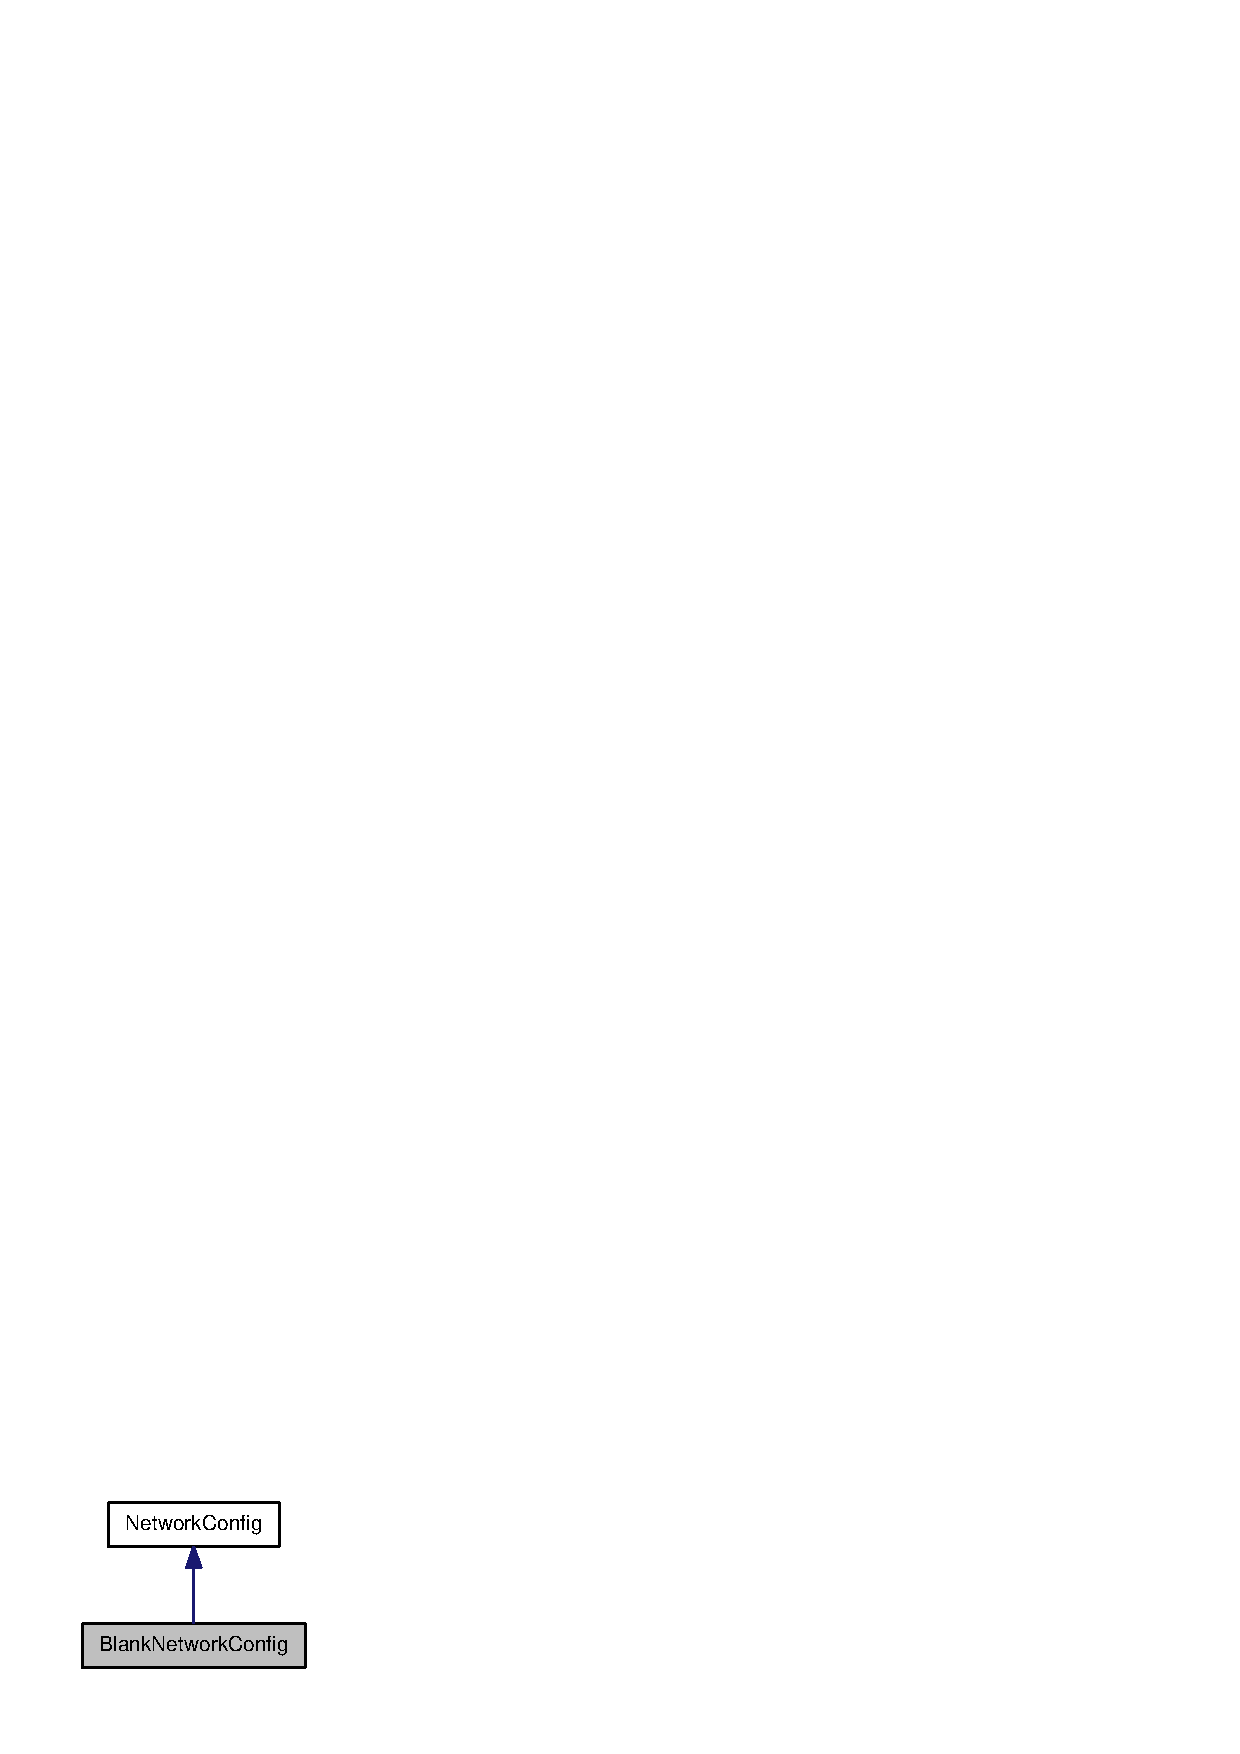
\includegraphics[width=150pt]{classBlankNetworkConfig__inherit__graph}
\end{center}
\end{figure}
\subsection*{\-Public \-Member \-Functions}
\begin{DoxyCompactItemize}
\item 
{\bf \-Blank\-Network\-Config} ()
\item 
virtual void {\bf update} (const \-Active\-Network\-Connections\-::\-Const\-Ptr active\-\_\-connections, {\bf \-Network\-Configuration\-Manager} $\ast$manager) const 
\item 
virtual {\bf $\sim$\-Blank\-Network\-Config} ()
\end{DoxyCompactItemize}


\subsection{\-Detailed \-Description}
\-A system network configuration which does nothing 

\-Definition at line 52 of file \-Network\-Configuration\-Manager.\-h.



\subsection{\-Constructor \& \-Destructor \-Documentation}
\index{\-Blank\-Network\-Config@{\-Blank\-Network\-Config}!\-Blank\-Network\-Config@{\-Blank\-Network\-Config}}
\index{\-Blank\-Network\-Config@{\-Blank\-Network\-Config}!BlankNetworkConfig@{\-Blank\-Network\-Config}}
\subsubsection[{\-Blank\-Network\-Config}]{\setlength{\rightskip}{0pt plus 5cm}{\bf \-Blank\-Network\-Config\-::\-Blank\-Network\-Config} (
\begin{DoxyParamCaption}
{}
\end{DoxyParamCaption}
)\hspace{0.3cm}{\ttfamily  [inline]}}\label{classBlankNetworkConfig_a6bf6f4fac7e3c858e48eefc051e74b30}


\-Definition at line 54 of file \-Network\-Configuration\-Manager.\-h.

\index{\-Blank\-Network\-Config@{\-Blank\-Network\-Config}!$\sim$\-Blank\-Network\-Config@{$\sim$\-Blank\-Network\-Config}}
\index{$\sim$\-Blank\-Network\-Config@{$\sim$\-Blank\-Network\-Config}!BlankNetworkConfig@{\-Blank\-Network\-Config}}
\subsubsection[{$\sim$\-Blank\-Network\-Config}]{\setlength{\rightskip}{0pt plus 5cm}virtual {\bf \-Blank\-Network\-Config\-::$\sim$\-Blank\-Network\-Config} (
\begin{DoxyParamCaption}
{}
\end{DoxyParamCaption}
)\hspace{0.3cm}{\ttfamily  [inline, virtual]}}\label{classBlankNetworkConfig_a95591fc933d9d34b30ec25af94440f47}


\-Definition at line 55 of file \-Network\-Configuration\-Manager.\-h.



\subsection{\-Member \-Function \-Documentation}
\index{\-Blank\-Network\-Config@{\-Blank\-Network\-Config}!update@{update}}
\index{update@{update}!BlankNetworkConfig@{\-Blank\-Network\-Config}}
\subsubsection[{update}]{\setlength{\rightskip}{0pt plus 5cm}virtual void {\bf \-Blank\-Network\-Config\-::update} (
\begin{DoxyParamCaption}
\item[{const \-Active\-Network\-Connections\-::\-Const\-Ptr}]{active\-\_\-connections, }
\item[{{\bf \-Network\-Configuration\-Manager} $\ast$}]{manager}
\end{DoxyParamCaption}
) const\hspace{0.3cm}{\ttfamily  [inline, virtual]}}\label{classBlankNetworkConfig_ac71e07a822f1c58fe95316b1a7f32bf2}


\-Reimplemented from {\bf \-Network\-Config} \doxyref{}{p.}{classNetworkConfig_aeee8e996f602b3447344f0edfbf9550f}.



\-Definition at line 56 of file \-Network\-Configuration\-Manager.\-h.



\-The documentation for this class was generated from the following file\-:\begin{DoxyCompactItemize}
\item 
{\bf \-Network\-Configuration\-Manager.\-h}\end{DoxyCompactItemize}

\section{\-Network\-Config \-Class \-Reference}
\label{classNetworkConfig}\index{\-Network\-Config@{\-Network\-Config}}


{\ttfamily \#include $<$\-Network\-Configuration\-Manager.\-h$>$}



\-Inheritance diagram for \-Network\-Config\-:
\nopagebreak
\begin{figure}[H]
\begin{center}
\leavevmode
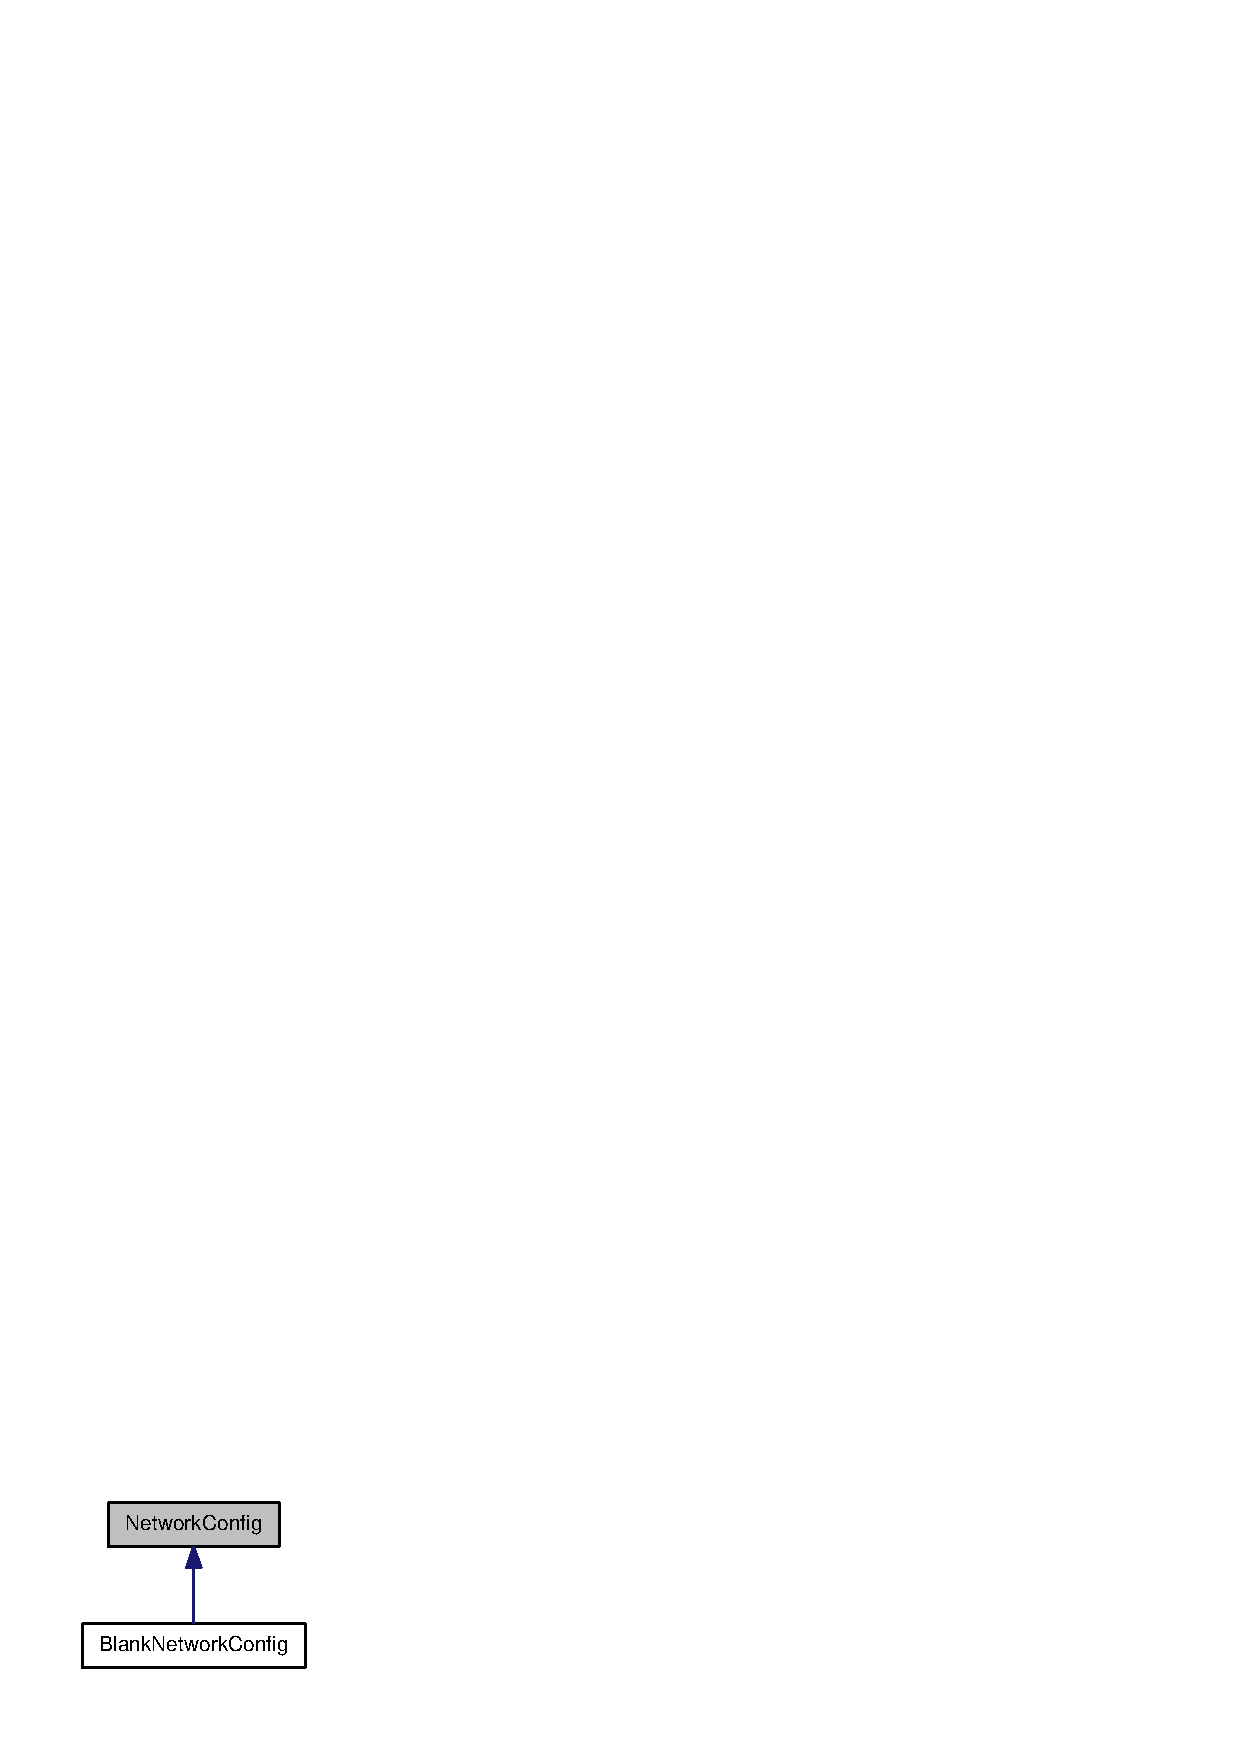
\includegraphics[width=150pt]{classNetworkConfig__inherit__graph}
\end{center}
\end{figure}
\subsection*{\-Public \-Member \-Functions}
\begin{DoxyCompactItemize}
\item 
const std\-::string {\bf get\-\_\-name} ()
\item 
{\bf \-Network\-Config} (std\-::string name, std\-::vector$<$ {\bf \-Network\-Connection\-Config} $>$ connection\-\_\-configs)
\item 
virtual void {\bf update} (const \-Active\-Network\-Connections\-::\-Const\-Ptr active\-\_\-connections, {\bf \-Network\-Configuration\-Manager} $\ast$manager) const 
\item 
virtual {\bf $\sim$\-Network\-Config} ()
\end{DoxyCompactItemize}
\subsection*{\-Private \-Attributes}
\begin{DoxyCompactItemize}
\item 
std\-::vector\*
$<$ {\bf \-Network\-Connection\-Config} $>$ {\bf m\-\_\-connection\-\_\-configs}
\item 
std\-::string {\bf m\-\_\-name}
\end{DoxyCompactItemize}


\subsection{\-Detailed \-Description}
\-A class which represents a system network configuration 

\-Definition at line 38 of file \-Network\-Configuration\-Manager.\-h.



\subsection{\-Constructor \& \-Destructor \-Documentation}
\index{\-Network\-Config@{\-Network\-Config}!\-Network\-Config@{\-Network\-Config}}
\index{\-Network\-Config@{\-Network\-Config}!NetworkConfig@{\-Network\-Config}}
\subsubsection[{\-Network\-Config}]{\setlength{\rightskip}{0pt plus 5cm}{\bf \-Network\-Config\-::\-Network\-Config} (
\begin{DoxyParamCaption}
\item[{std\-::string}]{name, }
\item[{std\-::vector$<$ {\bf \-Network\-Connection\-Config} $>$}]{connection\-\_\-configs}
\end{DoxyParamCaption}
)\hspace{0.3cm}{\ttfamily  [inline]}}\label{classNetworkConfig_ab4c049034717234c1c1d90a4a8b05889}


\-Definition at line 40 of file \-Network\-Configuration\-Manager.\-h.

\index{\-Network\-Config@{\-Network\-Config}!$\sim$\-Network\-Config@{$\sim$\-Network\-Config}}
\index{$\sim$\-Network\-Config@{$\sim$\-Network\-Config}!NetworkConfig@{\-Network\-Config}}
\subsubsection[{$\sim$\-Network\-Config}]{\setlength{\rightskip}{0pt plus 5cm}virtual {\bf \-Network\-Config\-::$\sim$\-Network\-Config} (
\begin{DoxyParamCaption}
{}
\end{DoxyParamCaption}
)\hspace{0.3cm}{\ttfamily  [inline, virtual]}}\label{classNetworkConfig_af1b02edd3f2cc8f0521c4c9f434fc8ec}


\-Definition at line 41 of file \-Network\-Configuration\-Manager.\-h.



\subsection{\-Member \-Function \-Documentation}
\index{\-Network\-Config@{\-Network\-Config}!get\-\_\-name@{get\-\_\-name}}
\index{get\-\_\-name@{get\-\_\-name}!NetworkConfig@{\-Network\-Config}}
\subsubsection[{get\-\_\-name}]{\setlength{\rightskip}{0pt plus 5cm}const std\-::string {\bf \-Network\-Config\-::get\-\_\-name} (
\begin{DoxyParamCaption}
{}
\end{DoxyParamCaption}
)\hspace{0.3cm}{\ttfamily  [inline]}}\label{classNetworkConfig_a04900c49193546025b845039ee3f4305}


\-Definition at line 43 of file \-Network\-Configuration\-Manager.\-h.

\index{\-Network\-Config@{\-Network\-Config}!update@{update}}
\index{update@{update}!NetworkConfig@{\-Network\-Config}}
\subsubsection[{update}]{\setlength{\rightskip}{0pt plus 5cm}void {\bf \-Network\-Config\-::update} (
\begin{DoxyParamCaption}
\item[{const \-Active\-Network\-Connections\-::\-Const\-Ptr}]{active\-\_\-connections, }
\item[{{\bf \-Network\-Configuration\-Manager} $\ast$}]{manager}
\end{DoxyParamCaption}
) const\hspace{0.3cm}{\ttfamily  [virtual]}}\label{classNetworkConfig_aeee8e996f602b3447344f0edfbf9550f}


\-Reimplemented in {\bf \-Blank\-Network\-Config} \doxyref{}{p.}{classBlankNetworkConfig_ac71e07a822f1c58fe95316b1a7f32bf2}.



\-Definition at line 100 of file \-Network\-Configuration\-Manager.\-cpp.



\subsection{\-Member \-Data \-Documentation}
\index{\-Network\-Config@{\-Network\-Config}!m\-\_\-connection\-\_\-configs@{m\-\_\-connection\-\_\-configs}}
\index{m\-\_\-connection\-\_\-configs@{m\-\_\-connection\-\_\-configs}!NetworkConfig@{\-Network\-Config}}
\subsubsection[{m\-\_\-connection\-\_\-configs}]{\setlength{\rightskip}{0pt plus 5cm}std\-::vector$<${\bf \-Network\-Connection\-Config}$>$ {\bf \-Network\-Config\-::m\-\_\-connection\-\_\-configs}\hspace{0.3cm}{\ttfamily  [private]}}\label{classNetworkConfig_ab8d1837519d4bd6e391ccce1fde01c83}


\-Definition at line 46 of file \-Network\-Configuration\-Manager.\-h.

\index{\-Network\-Config@{\-Network\-Config}!m\-\_\-name@{m\-\_\-name}}
\index{m\-\_\-name@{m\-\_\-name}!NetworkConfig@{\-Network\-Config}}
\subsubsection[{m\-\_\-name}]{\setlength{\rightskip}{0pt plus 5cm}std\-::string {\bf \-Network\-Config\-::m\-\_\-name}\hspace{0.3cm}{\ttfamily  [private]}}\label{classNetworkConfig_afc1a2af677203f3df889b19984571309}


\-Definition at line 43 of file \-Network\-Configuration\-Manager.\-h.



\-The documentation for this class was generated from the following files\-:\begin{DoxyCompactItemize}
\item 
{\bf \-Network\-Configuration\-Manager.\-h}\item 
{\bf \-Network\-Configuration\-Manager.\-cpp}\end{DoxyCompactItemize}

\section{\-Network\-Configuration\-Manager \-Class \-Reference}
\label{classNetworkConfigurationManager}\index{\-Network\-Configuration\-Manager@{\-Network\-Configuration\-Manager}}


{\ttfamily \#include $<$\-Network\-Configuration\-Manager.\-h$>$}

\subsection*{\-Public \-Member \-Functions}
\begin{DoxyCompactItemize}
\item 
bool {\bf activate\-\_\-connection} (std\-::string iface, std\-::string connection\-\_\-name)
\item 
void {\bf load\-\_\-config\-\_\-from\-\_\-file} (const char $\ast$filename)
\item 
{\bf \-Network\-Configuration\-Manager} (ros\-::\-Node\-Handle \&handle, \-N\-M\-Client $\ast$client, \-N\-M\-Remote\-Settings $\ast$remote\-\_\-settings)
\item 
void {\bf set\-\_\-config} (boost\-::shared\-\_\-ptr$<$ {\bf \-Network\-Config} $>$ new\-\_\-config)
\item 
virtual {\bf $\sim$\-Network\-Configuration\-Manager} ()
\end{DoxyCompactItemize}
\subsection*{\-Private \-Member \-Functions}
\begin{DoxyCompactItemize}
\item 
void {\bf active\-\_\-connections\-\_\-changed\-\_\-cb} (const \-Active\-Network\-Connections\-::\-Const\-Ptr \&latest\-\_\-connections)
\item 
void {\bf connections\-\_\-changed\-\_\-cb} (const \-Network\-Connections\-::\-Const\-Ptr \&latest\-\_\-connections)
\item 
void {\bf update\-\_\-config} ()
\end{DoxyCompactItemize}
\subsection*{\-Private \-Attributes}
\begin{DoxyCompactItemize}
\item 
ros\-::\-Subscriber {\bf active\-\_\-connection\-\_\-sub}
\item 
ros\-::\-Subscriber {\bf connection\-\_\-sub}
\item 
\-N\-M\-Client $\ast$ {\bf m\-\_\-client}
\item 
boost\-::shared\-\_\-ptr$<$ {\bf \-Network\-Config} $>$ {\bf m\-\_\-config}
\item 
ros\-::\-Node\-Handle \& {\bf m\-\_\-handle}
\item 
\-Active\-Network\-Connections\-::\-Const\-Ptr {\bf m\-\_\-latest\-\_\-active\-\_\-connections}
\item 
\-Network\-Connections\-::\-Const\-Ptr {\bf m\-\_\-latest\-\_\-connections}
\item 
\-N\-M\-Remote\-Settings $\ast$ {\bf m\-\_\-remote\-\_\-settings}
\end{DoxyCompactItemize}


\subsection{\-Detailed \-Description}
\-A class which manages the the active configuration 

\-Definition at line 62 of file \-Network\-Configuration\-Manager.\-h.



\subsection{\-Constructor \& \-Destructor \-Documentation}
\index{\-Network\-Configuration\-Manager@{\-Network\-Configuration\-Manager}!\-Network\-Configuration\-Manager@{\-Network\-Configuration\-Manager}}
\index{\-Network\-Configuration\-Manager@{\-Network\-Configuration\-Manager}!NetworkConfigurationManager@{\-Network\-Configuration\-Manager}}
\subsubsection[{\-Network\-Configuration\-Manager}]{\setlength{\rightskip}{0pt plus 5cm}{\bf \-Network\-Configuration\-Manager\-::\-Network\-Configuration\-Manager} (
\begin{DoxyParamCaption}
\item[{ros\-::\-Node\-Handle \&}]{handle, }
\item[{\-N\-M\-Client $\ast$}]{client, }
\item[{\-N\-M\-Remote\-Settings $\ast$}]{remote\-\_\-settings}
\end{DoxyParamCaption}
)}\label{classNetworkConfigurationManager_a64ae8256fb391ee0488432685501fa4f}


\-Definition at line 11 of file \-Network\-Configuration\-Manager.\-cpp.

\index{\-Network\-Configuration\-Manager@{\-Network\-Configuration\-Manager}!$\sim$\-Network\-Configuration\-Manager@{$\sim$\-Network\-Configuration\-Manager}}
\index{$\sim$\-Network\-Configuration\-Manager@{$\sim$\-Network\-Configuration\-Manager}!NetworkConfigurationManager@{\-Network\-Configuration\-Manager}}
\subsubsection[{$\sim$\-Network\-Configuration\-Manager}]{\setlength{\rightskip}{0pt plus 5cm}{\bf \-Network\-Configuration\-Manager\-::$\sim$\-Network\-Configuration\-Manager} (
\begin{DoxyParamCaption}
{}
\end{DoxyParamCaption}
)\hspace{0.3cm}{\ttfamily  [virtual]}}\label{classNetworkConfigurationManager_a986f55ebf2c2b37b09b45b297ec5c2b8}


\-Definition at line 166 of file \-Network\-Configuration\-Manager.\-cpp.



\subsection{\-Member \-Function \-Documentation}
\index{\-Network\-Configuration\-Manager@{\-Network\-Configuration\-Manager}!activate\-\_\-connection@{activate\-\_\-connection}}
\index{activate\-\_\-connection@{activate\-\_\-connection}!NetworkConfigurationManager@{\-Network\-Configuration\-Manager}}
\subsubsection[{activate\-\_\-connection}]{\setlength{\rightskip}{0pt plus 5cm}bool {\bf \-Network\-Configuration\-Manager\-::activate\-\_\-connection} (
\begin{DoxyParamCaption}
\item[{std\-::string}]{iface, }
\item[{std\-::string}]{connection\-\_\-name}
\end{DoxyParamCaption}
)}\label{classNetworkConfigurationManager_ac53a0cefb1945574af3fa46e6846b6e0}


\-Definition at line 123 of file \-Network\-Configuration\-Manager.\-cpp.

\index{\-Network\-Configuration\-Manager@{\-Network\-Configuration\-Manager}!active\-\_\-connections\-\_\-changed\-\_\-cb@{active\-\_\-connections\-\_\-changed\-\_\-cb}}
\index{active\-\_\-connections\-\_\-changed\-\_\-cb@{active\-\_\-connections\-\_\-changed\-\_\-cb}!NetworkConfigurationManager@{\-Network\-Configuration\-Manager}}
\subsubsection[{active\-\_\-connections\-\_\-changed\-\_\-cb}]{\setlength{\rightskip}{0pt plus 5cm}void {\bf \-Network\-Configuration\-Manager\-::active\-\_\-connections\-\_\-changed\-\_\-cb} (
\begin{DoxyParamCaption}
\item[{const \-Active\-Network\-Connections\-::\-Const\-Ptr \&}]{latest\-\_\-connections}
\end{DoxyParamCaption}
)\hspace{0.3cm}{\ttfamily  [private]}}\label{classNetworkConfigurationManager_ae1339a0032203c62409286b6ec2f8362}


\-Definition at line 74 of file \-Network\-Configuration\-Manager.\-cpp.

\index{\-Network\-Configuration\-Manager@{\-Network\-Configuration\-Manager}!connections\-\_\-changed\-\_\-cb@{connections\-\_\-changed\-\_\-cb}}
\index{connections\-\_\-changed\-\_\-cb@{connections\-\_\-changed\-\_\-cb}!NetworkConfigurationManager@{\-Network\-Configuration\-Manager}}
\subsubsection[{connections\-\_\-changed\-\_\-cb}]{\setlength{\rightskip}{0pt plus 5cm}void {\bf \-Network\-Configuration\-Manager\-::connections\-\_\-changed\-\_\-cb} (
\begin{DoxyParamCaption}
\item[{const \-Network\-Connections\-::\-Const\-Ptr \&}]{latest\-\_\-connections}
\end{DoxyParamCaption}
)\hspace{0.3cm}{\ttfamily  [private]}}\label{classNetworkConfigurationManager_ab254b7f93bd4624210852aac1d8f21e4}


\-Definition at line 80 of file \-Network\-Configuration\-Manager.\-cpp.

\index{\-Network\-Configuration\-Manager@{\-Network\-Configuration\-Manager}!load\-\_\-config\-\_\-from\-\_\-file@{load\-\_\-config\-\_\-from\-\_\-file}}
\index{load\-\_\-config\-\_\-from\-\_\-file@{load\-\_\-config\-\_\-from\-\_\-file}!NetworkConfigurationManager@{\-Network\-Configuration\-Manager}}
\subsubsection[{load\-\_\-config\-\_\-from\-\_\-file}]{\setlength{\rightskip}{0pt plus 5cm}void {\bf \-Network\-Configuration\-Manager\-::load\-\_\-config\-\_\-from\-\_\-file} (
\begin{DoxyParamCaption}
\item[{const char $\ast$}]{filename}
\end{DoxyParamCaption}
)}\label{classNetworkConfigurationManager_a2718c71af598abdd08014ef6e3b7948b}


\-Definition at line 22 of file \-Network\-Configuration\-Manager.\-cpp.

\index{\-Network\-Configuration\-Manager@{\-Network\-Configuration\-Manager}!set\-\_\-config@{set\-\_\-config}}
\index{set\-\_\-config@{set\-\_\-config}!NetworkConfigurationManager@{\-Network\-Configuration\-Manager}}
\subsubsection[{set\-\_\-config}]{\setlength{\rightskip}{0pt plus 5cm}void {\bf \-Network\-Configuration\-Manager\-::set\-\_\-config} (
\begin{DoxyParamCaption}
\item[{boost\-::shared\-\_\-ptr$<$ {\bf \-Network\-Config} $>$}]{new\-\_\-config}
\end{DoxyParamCaption}
)}\label{classNetworkConfigurationManager_af2d14623dcbcbc57a4acabbd70eb75e0}


\-Definition at line 67 of file \-Network\-Configuration\-Manager.\-cpp.

\index{\-Network\-Configuration\-Manager@{\-Network\-Configuration\-Manager}!update\-\_\-config@{update\-\_\-config}}
\index{update\-\_\-config@{update\-\_\-config}!NetworkConfigurationManager@{\-Network\-Configuration\-Manager}}
\subsubsection[{update\-\_\-config}]{\setlength{\rightskip}{0pt plus 5cm}void {\bf \-Network\-Configuration\-Manager\-::update\-\_\-config} (
\begin{DoxyParamCaption}
{}
\end{DoxyParamCaption}
)\hspace{0.3cm}{\ttfamily  [private]}}\label{classNetworkConfigurationManager_a6b16703c640ab8598a9c0fe7ca84ed2c}


\-Definition at line 85 of file \-Network\-Configuration\-Manager.\-cpp.



\subsection{\-Member \-Data \-Documentation}
\index{\-Network\-Configuration\-Manager@{\-Network\-Configuration\-Manager}!active\-\_\-connection\-\_\-sub@{active\-\_\-connection\-\_\-sub}}
\index{active\-\_\-connection\-\_\-sub@{active\-\_\-connection\-\_\-sub}!NetworkConfigurationManager@{\-Network\-Configuration\-Manager}}
\subsubsection[{active\-\_\-connection\-\_\-sub}]{\setlength{\rightskip}{0pt plus 5cm}ros\-::\-Subscriber {\bf \-Network\-Configuration\-Manager\-::active\-\_\-connection\-\_\-sub}\hspace{0.3cm}{\ttfamily  [private]}}\label{classNetworkConfigurationManager_a87f5f5864731d45b3ad342445f1e081c}


\-Definition at line 80 of file \-Network\-Configuration\-Manager.\-h.

\index{\-Network\-Configuration\-Manager@{\-Network\-Configuration\-Manager}!connection\-\_\-sub@{connection\-\_\-sub}}
\index{connection\-\_\-sub@{connection\-\_\-sub}!NetworkConfigurationManager@{\-Network\-Configuration\-Manager}}
\subsubsection[{connection\-\_\-sub}]{\setlength{\rightskip}{0pt plus 5cm}ros\-::\-Subscriber {\bf \-Network\-Configuration\-Manager\-::connection\-\_\-sub}\hspace{0.3cm}{\ttfamily  [private]}}\label{classNetworkConfigurationManager_a6ce6469d5de5bc935062c3902bf57ae0}


\-Definition at line 78 of file \-Network\-Configuration\-Manager.\-h.

\index{\-Network\-Configuration\-Manager@{\-Network\-Configuration\-Manager}!m\-\_\-client@{m\-\_\-client}}
\index{m\-\_\-client@{m\-\_\-client}!NetworkConfigurationManager@{\-Network\-Configuration\-Manager}}
\subsubsection[{m\-\_\-client}]{\setlength{\rightskip}{0pt plus 5cm}\-N\-M\-Client$\ast$ {\bf \-Network\-Configuration\-Manager\-::m\-\_\-client}\hspace{0.3cm}{\ttfamily  [private]}}\label{classNetworkConfigurationManager_ad3e7ab11c29f836976fa4432c069fadc}


\-Definition at line 76 of file \-Network\-Configuration\-Manager.\-h.

\index{\-Network\-Configuration\-Manager@{\-Network\-Configuration\-Manager}!m\-\_\-config@{m\-\_\-config}}
\index{m\-\_\-config@{m\-\_\-config}!NetworkConfigurationManager@{\-Network\-Configuration\-Manager}}
\subsubsection[{m\-\_\-config}]{\setlength{\rightskip}{0pt plus 5cm}boost\-::shared\-\_\-ptr$<${\bf \-Network\-Config}$>$ {\bf \-Network\-Configuration\-Manager\-::m\-\_\-config}\hspace{0.3cm}{\ttfamily  [private]}}\label{classNetworkConfigurationManager_a13e746bf1caed53802c1abc6d84039cc}


\-Definition at line 82 of file \-Network\-Configuration\-Manager.\-h.

\index{\-Network\-Configuration\-Manager@{\-Network\-Configuration\-Manager}!m\-\_\-handle@{m\-\_\-handle}}
\index{m\-\_\-handle@{m\-\_\-handle}!NetworkConfigurationManager@{\-Network\-Configuration\-Manager}}
\subsubsection[{m\-\_\-handle}]{\setlength{\rightskip}{0pt plus 5cm}ros\-::\-Node\-Handle\& {\bf \-Network\-Configuration\-Manager\-::m\-\_\-handle}\hspace{0.3cm}{\ttfamily  [private]}}\label{classNetworkConfigurationManager_ab5f5fb7e24e1c58738cfc8b976557248}


\-Definition at line 75 of file \-Network\-Configuration\-Manager.\-h.

\index{\-Network\-Configuration\-Manager@{\-Network\-Configuration\-Manager}!m\-\_\-latest\-\_\-active\-\_\-connections@{m\-\_\-latest\-\_\-active\-\_\-connections}}
\index{m\-\_\-latest\-\_\-active\-\_\-connections@{m\-\_\-latest\-\_\-active\-\_\-connections}!NetworkConfigurationManager@{\-Network\-Configuration\-Manager}}
\subsubsection[{m\-\_\-latest\-\_\-active\-\_\-connections}]{\setlength{\rightskip}{0pt plus 5cm}\-Active\-Network\-Connections\-::\-Const\-Ptr {\bf \-Network\-Configuration\-Manager\-::m\-\_\-latest\-\_\-active\-\_\-connections}\hspace{0.3cm}{\ttfamily  [private]}}\label{classNetworkConfigurationManager_a3363ab3b2d8369ff5ca376d7834036ff}


\-Definition at line 81 of file \-Network\-Configuration\-Manager.\-h.

\index{\-Network\-Configuration\-Manager@{\-Network\-Configuration\-Manager}!m\-\_\-latest\-\_\-connections@{m\-\_\-latest\-\_\-connections}}
\index{m\-\_\-latest\-\_\-connections@{m\-\_\-latest\-\_\-connections}!NetworkConfigurationManager@{\-Network\-Configuration\-Manager}}
\subsubsection[{m\-\_\-latest\-\_\-connections}]{\setlength{\rightskip}{0pt plus 5cm}\-Network\-Connections\-::\-Const\-Ptr {\bf \-Network\-Configuration\-Manager\-::m\-\_\-latest\-\_\-connections}\hspace{0.3cm}{\ttfamily  [private]}}\label{classNetworkConfigurationManager_adc1dc81d476f0db5375ad69da8b4add4}


\-Definition at line 79 of file \-Network\-Configuration\-Manager.\-h.

\index{\-Network\-Configuration\-Manager@{\-Network\-Configuration\-Manager}!m\-\_\-remote\-\_\-settings@{m\-\_\-remote\-\_\-settings}}
\index{m\-\_\-remote\-\_\-settings@{m\-\_\-remote\-\_\-settings}!NetworkConfigurationManager@{\-Network\-Configuration\-Manager}}
\subsubsection[{m\-\_\-remote\-\_\-settings}]{\setlength{\rightskip}{0pt plus 5cm}\-N\-M\-Remote\-Settings$\ast$ {\bf \-Network\-Configuration\-Manager\-::m\-\_\-remote\-\_\-settings}\hspace{0.3cm}{\ttfamily  [private]}}\label{classNetworkConfigurationManager_a4e74292e88e07caebee36c7a6fba78f9}


\-Definition at line 77 of file \-Network\-Configuration\-Manager.\-h.



\-The documentation for this class was generated from the following files\-:\begin{DoxyCompactItemize}
\item 
{\bf \-Network\-Configuration\-Manager.\-h}\item 
{\bf \-Network\-Configuration\-Manager.\-cpp}\end{DoxyCompactItemize}

\section{\-Network\-Connection\-Config \-Class \-Reference}
\label{classNetworkConnectionConfig}\index{\-Network\-Connection\-Config@{\-Network\-Connection\-Config}}


{\ttfamily \#include $<$\-Network\-Configuration\-Manager.\-h$>$}

\subsection*{\-Public \-Member \-Functions}
\begin{DoxyCompactItemize}
\item 
{\bf \-Network\-Connection\-Config} (std\-::string iface, std\-::string connection\-\_\-name)
\item 
virtual void {\bf update} (const \-Active\-Network\-Connections\-::\-Const\-Ptr active\-\_\-connections, {\bf \-Network\-Configuration\-Manager} $\ast$manager) const 
\item 
virtual {\bf $\sim$\-Network\-Connection\-Config} ()
\end{DoxyCompactItemize}
\subsection*{\-Private \-Attributes}
\begin{DoxyCompactItemize}
\item 
std\-::string {\bf m\-\_\-connection\-\_\-name}
\item 
std\-::string {\bf m\-\_\-iface}
\end{DoxyCompactItemize}


\subsection{\-Detailed \-Description}
\-A configuration which outlines how a connection will be connected 

\-Definition at line 26 of file \-Network\-Configuration\-Manager.\-h.



\subsection{\-Constructor \& \-Destructor \-Documentation}
\index{\-Network\-Connection\-Config@{\-Network\-Connection\-Config}!\-Network\-Connection\-Config@{\-Network\-Connection\-Config}}
\index{\-Network\-Connection\-Config@{\-Network\-Connection\-Config}!NetworkConnectionConfig@{\-Network\-Connection\-Config}}
\subsubsection[{\-Network\-Connection\-Config}]{\setlength{\rightskip}{0pt plus 5cm}{\bf \-Network\-Connection\-Config\-::\-Network\-Connection\-Config} (
\begin{DoxyParamCaption}
\item[{std\-::string}]{iface, }
\item[{std\-::string}]{connection\-\_\-name}
\end{DoxyParamCaption}
)\hspace{0.3cm}{\ttfamily  [inline]}}\label{classNetworkConnectionConfig_a811f2ce03882f03eaec22ef36b52a20a}


\-Definition at line 28 of file \-Network\-Configuration\-Manager.\-h.

\index{\-Network\-Connection\-Config@{\-Network\-Connection\-Config}!$\sim$\-Network\-Connection\-Config@{$\sim$\-Network\-Connection\-Config}}
\index{$\sim$\-Network\-Connection\-Config@{$\sim$\-Network\-Connection\-Config}!NetworkConnectionConfig@{\-Network\-Connection\-Config}}
\subsubsection[{$\sim$\-Network\-Connection\-Config}]{\setlength{\rightskip}{0pt plus 5cm}virtual {\bf \-Network\-Connection\-Config\-::$\sim$\-Network\-Connection\-Config} (
\begin{DoxyParamCaption}
{}
\end{DoxyParamCaption}
)\hspace{0.3cm}{\ttfamily  [inline, virtual]}}\label{classNetworkConnectionConfig_a54c0a49a0cb124de40fa2a2203dca03d}


\-Definition at line 29 of file \-Network\-Configuration\-Manager.\-h.



\subsection{\-Member \-Function \-Documentation}
\index{\-Network\-Connection\-Config@{\-Network\-Connection\-Config}!update@{update}}
\index{update@{update}!NetworkConnectionConfig@{\-Network\-Connection\-Config}}
\subsubsection[{update}]{\setlength{\rightskip}{0pt plus 5cm}void {\bf \-Network\-Connection\-Config\-::update} (
\begin{DoxyParamCaption}
\item[{const \-Active\-Network\-Connections\-::\-Const\-Ptr}]{active\-\_\-connections, }
\item[{{\bf \-Network\-Configuration\-Manager} $\ast$}]{manager}
\end{DoxyParamCaption}
) const\hspace{0.3cm}{\ttfamily  [virtual]}}\label{classNetworkConnectionConfig_afca8b3a0328019defab6c11d97c17f11}


\-Definition at line 106 of file \-Network\-Configuration\-Manager.\-cpp.



\subsection{\-Member \-Data \-Documentation}
\index{\-Network\-Connection\-Config@{\-Network\-Connection\-Config}!m\-\_\-connection\-\_\-name@{m\-\_\-connection\-\_\-name}}
\index{m\-\_\-connection\-\_\-name@{m\-\_\-connection\-\_\-name}!NetworkConnectionConfig@{\-Network\-Connection\-Config}}
\subsubsection[{m\-\_\-connection\-\_\-name}]{\setlength{\rightskip}{0pt plus 5cm}std\-::string {\bf \-Network\-Connection\-Config\-::m\-\_\-connection\-\_\-name}\hspace{0.3cm}{\ttfamily  [private]}}\label{classNetworkConnectionConfig_a2e287665f93f21d4f8d6398965b92e12}


\-Definition at line 33 of file \-Network\-Configuration\-Manager.\-h.

\index{\-Network\-Connection\-Config@{\-Network\-Connection\-Config}!m\-\_\-iface@{m\-\_\-iface}}
\index{m\-\_\-iface@{m\-\_\-iface}!NetworkConnectionConfig@{\-Network\-Connection\-Config}}
\subsubsection[{m\-\_\-iface}]{\setlength{\rightskip}{0pt plus 5cm}std\-::string {\bf \-Network\-Connection\-Config\-::m\-\_\-iface}\hspace{0.3cm}{\ttfamily  [private]}}\label{classNetworkConnectionConfig_a7b71395d73455b55aa554c948ccd8dfa}


\-Definition at line 32 of file \-Network\-Configuration\-Manager.\-h.



\-The documentation for this class was generated from the following files\-:\begin{DoxyCompactItemize}
\item 
{\bf \-Network\-Configuration\-Manager.\-h}\item 
{\bf \-Network\-Configuration\-Manager.\-cpp}\end{DoxyCompactItemize}

\section{\-Network\-Connection\-Manager \-Class \-Reference}
\label{classNetworkConnectionManager}\index{\-Network\-Connection\-Manager@{\-Network\-Connection\-Manager}}


{\ttfamily \#include $<$\-Network\-Connection\-Manager.\-h$>$}

\subsection*{\-Public \-Member \-Functions}
\begin{DoxyCompactItemize}
\item 
{\bf \-Network\-Connection\-Manager} (ros\-::\-Node\-Handle \&handle, \-N\-M\-Remote\-Settings $\ast$remote\-\_\-settings)
\item 
virtual {\bf $\sim$\-Network\-Connection\-Manager} ()
\end{DoxyCompactItemize}
\subsection*{\-Private \-Member \-Functions}
\begin{DoxyCompactItemize}
\item 
void {\bf fill\-\_\-connection\-\_\-info} (\-N\-M\-Connection $\ast$connection, oryx\-\_\-network\-\_\-manager\-::\-Network\-Connection \&ros\-\_\-connection\-\_\-message)
\item 
void {\bf process\-\_\-added\-\_\-connection} (\-N\-M\-Connection $\ast$connection)
\item 
void {\bf process\-\_\-removed\-\_\-connection} (\-N\-M\-Connection $\ast$connection)
\item 
void {\bf process\-\_\-updated\-\_\-connection} (\-N\-M\-Connection $\ast$connection)
\item 
void {\bf publish\-\_\-connections} ()
\end{DoxyCompactItemize}
\subsection*{\-Static \-Private \-Member \-Functions}
\begin{DoxyCompactItemize}
\item 
static void {\bf connection\-\_\-added\-\_\-cb} (\-N\-M\-Remote\-Settings $\ast$settings, \-N\-M\-Remote\-Connection $\ast$connection, gpointer user\-\_\-data)
\item 
static void {\bf connection\-\_\-removed\-\_\-cb} (\-N\-M\-Remote\-Connection $\ast$connection, gpointer user\-\_\-data)
\item 
static void {\bf connection\-\_\-updated\-\_\-cb} (\-N\-M\-Remote\-Connection $\ast$connection, gpointer user\-\_\-data)
\end{DoxyCompactItemize}
\subsection*{\-Private \-Attributes}
\begin{DoxyCompactItemize}
\item 
ros\-::\-Publisher {\bf connection\-\_\-pub}
\item 
std\-::map$<$ std\-::string, \*
\-Network\-Connection $>$ {\bf connections}
\item 
ros\-::\-Node\-Handle \& {\bf m\-\_\-handle}
\item 
\-N\-M\-Remote\-Settings $\ast$ {\bf m\-\_\-remote\-\_\-settings}
\item 
uint32\-\_\-t {\bf msg\-\_\-seq}
\end{DoxyCompactItemize}


\subsection{\-Detailed \-Description}


\-Definition at line 20 of file \-Network\-Connection\-Manager.\-h.



\subsection{\-Constructor \& \-Destructor \-Documentation}
\index{\-Network\-Connection\-Manager@{\-Network\-Connection\-Manager}!\-Network\-Connection\-Manager@{\-Network\-Connection\-Manager}}
\index{\-Network\-Connection\-Manager@{\-Network\-Connection\-Manager}!NetworkConnectionManager@{\-Network\-Connection\-Manager}}
\subsubsection[{\-Network\-Connection\-Manager}]{\setlength{\rightskip}{0pt plus 5cm}{\bf \-Network\-Connection\-Manager\-::\-Network\-Connection\-Manager} (
\begin{DoxyParamCaption}
\item[{ros\-::\-Node\-Handle \&}]{handle, }
\item[{\-N\-M\-Remote\-Settings $\ast$}]{remote\-\_\-settings}
\end{DoxyParamCaption}
)}\label{classNetworkConnectionManager_af691594031396547501dd0907b710ee2}


\-Definition at line 15 of file \-Network\-Connection\-Manager.\-cpp.

\index{\-Network\-Connection\-Manager@{\-Network\-Connection\-Manager}!$\sim$\-Network\-Connection\-Manager@{$\sim$\-Network\-Connection\-Manager}}
\index{$\sim$\-Network\-Connection\-Manager@{$\sim$\-Network\-Connection\-Manager}!NetworkConnectionManager@{\-Network\-Connection\-Manager}}
\subsubsection[{$\sim$\-Network\-Connection\-Manager}]{\setlength{\rightskip}{0pt plus 5cm}{\bf \-Network\-Connection\-Manager\-::$\sim$\-Network\-Connection\-Manager} (
\begin{DoxyParamCaption}
{}
\end{DoxyParamCaption}
)\hspace{0.3cm}{\ttfamily  [virtual]}}\label{classNetworkConnectionManager_a678b84c10e82b3a71b04412a445cf086}


\-Definition at line 142 of file \-Network\-Connection\-Manager.\-cpp.



\subsection{\-Member \-Function \-Documentation}
\index{\-Network\-Connection\-Manager@{\-Network\-Connection\-Manager}!connection\-\_\-added\-\_\-cb@{connection\-\_\-added\-\_\-cb}}
\index{connection\-\_\-added\-\_\-cb@{connection\-\_\-added\-\_\-cb}!NetworkConnectionManager@{\-Network\-Connection\-Manager}}
\subsubsection[{connection\-\_\-added\-\_\-cb}]{\setlength{\rightskip}{0pt plus 5cm}void {\bf \-Network\-Connection\-Manager\-::connection\-\_\-added\-\_\-cb} (
\begin{DoxyParamCaption}
\item[{\-N\-M\-Remote\-Settings $\ast$}]{settings, }
\item[{\-N\-M\-Remote\-Connection $\ast$}]{connection, }
\item[{gpointer}]{user\-\_\-data}
\end{DoxyParamCaption}
)\hspace{0.3cm}{\ttfamily  [static, private]}}\label{classNetworkConnectionManager_a1dd8e0c5ef18b8d408130488e9fdd73f}


\-Definition at line 125 of file \-Network\-Connection\-Manager.\-cpp.

\index{\-Network\-Connection\-Manager@{\-Network\-Connection\-Manager}!connection\-\_\-removed\-\_\-cb@{connection\-\_\-removed\-\_\-cb}}
\index{connection\-\_\-removed\-\_\-cb@{connection\-\_\-removed\-\_\-cb}!NetworkConnectionManager@{\-Network\-Connection\-Manager}}
\subsubsection[{connection\-\_\-removed\-\_\-cb}]{\setlength{\rightskip}{0pt plus 5cm}void {\bf \-Network\-Connection\-Manager\-::connection\-\_\-removed\-\_\-cb} (
\begin{DoxyParamCaption}
\item[{\-N\-M\-Remote\-Connection $\ast$}]{connection, }
\item[{gpointer}]{user\-\_\-data}
\end{DoxyParamCaption}
)\hspace{0.3cm}{\ttfamily  [static, private]}}\label{classNetworkConnectionManager_a768b30e75063ea029cf8857771d977c7}


\-Definition at line 131 of file \-Network\-Connection\-Manager.\-cpp.

\index{\-Network\-Connection\-Manager@{\-Network\-Connection\-Manager}!connection\-\_\-updated\-\_\-cb@{connection\-\_\-updated\-\_\-cb}}
\index{connection\-\_\-updated\-\_\-cb@{connection\-\_\-updated\-\_\-cb}!NetworkConnectionManager@{\-Network\-Connection\-Manager}}
\subsubsection[{connection\-\_\-updated\-\_\-cb}]{\setlength{\rightskip}{0pt plus 5cm}void {\bf \-Network\-Connection\-Manager\-::connection\-\_\-updated\-\_\-cb} (
\begin{DoxyParamCaption}
\item[{\-N\-M\-Remote\-Connection $\ast$}]{connection, }
\item[{gpointer}]{user\-\_\-data}
\end{DoxyParamCaption}
)\hspace{0.3cm}{\ttfamily  [static, private]}}\label{classNetworkConnectionManager_a999bede48c73a0a731edfa2659acc2e6}


\-Definition at line 136 of file \-Network\-Connection\-Manager.\-cpp.

\index{\-Network\-Connection\-Manager@{\-Network\-Connection\-Manager}!fill\-\_\-connection\-\_\-info@{fill\-\_\-connection\-\_\-info}}
\index{fill\-\_\-connection\-\_\-info@{fill\-\_\-connection\-\_\-info}!NetworkConnectionManager@{\-Network\-Connection\-Manager}}
\subsubsection[{fill\-\_\-connection\-\_\-info}]{\setlength{\rightskip}{0pt plus 5cm}void {\bf \-Network\-Connection\-Manager\-::fill\-\_\-connection\-\_\-info} (
\begin{DoxyParamCaption}
\item[{\-N\-M\-Connection $\ast$}]{connection, }
\item[{oryx\-\_\-network\-\_\-manager\-::\-Network\-Connection \&}]{ros\-\_\-connection\-\_\-message}
\end{DoxyParamCaption}
)\hspace{0.3cm}{\ttfamily  [private]}}\label{classNetworkConnectionManager_a83f9554139aa38ff8677c458505c2868}


\-Definition at line 56 of file \-Network\-Connection\-Manager.\-cpp.

\index{\-Network\-Connection\-Manager@{\-Network\-Connection\-Manager}!process\-\_\-added\-\_\-connection@{process\-\_\-added\-\_\-connection}}
\index{process\-\_\-added\-\_\-connection@{process\-\_\-added\-\_\-connection}!NetworkConnectionManager@{\-Network\-Connection\-Manager}}
\subsubsection[{process\-\_\-added\-\_\-connection}]{\setlength{\rightskip}{0pt plus 5cm}void {\bf \-Network\-Connection\-Manager\-::process\-\_\-added\-\_\-connection} (
\begin{DoxyParamCaption}
\item[{\-N\-M\-Connection $\ast$}]{connection}
\end{DoxyParamCaption}
)\hspace{0.3cm}{\ttfamily  [private]}}\label{classNetworkConnectionManager_ae4bcc03b4cdd03c8905684435989e959}


\-Definition at line 24 of file \-Network\-Connection\-Manager.\-cpp.

\index{\-Network\-Connection\-Manager@{\-Network\-Connection\-Manager}!process\-\_\-removed\-\_\-connection@{process\-\_\-removed\-\_\-connection}}
\index{process\-\_\-removed\-\_\-connection@{process\-\_\-removed\-\_\-connection}!NetworkConnectionManager@{\-Network\-Connection\-Manager}}
\subsubsection[{process\-\_\-removed\-\_\-connection}]{\setlength{\rightskip}{0pt plus 5cm}void {\bf \-Network\-Connection\-Manager\-::process\-\_\-removed\-\_\-connection} (
\begin{DoxyParamCaption}
\item[{\-N\-M\-Connection $\ast$}]{connection}
\end{DoxyParamCaption}
)\hspace{0.3cm}{\ttfamily  [private]}}\label{classNetworkConnectionManager_afd8068d0716e0a43080ee86778a4d5b2}


\-Definition at line 36 of file \-Network\-Connection\-Manager.\-cpp.

\index{\-Network\-Connection\-Manager@{\-Network\-Connection\-Manager}!process\-\_\-updated\-\_\-connection@{process\-\_\-updated\-\_\-connection}}
\index{process\-\_\-updated\-\_\-connection@{process\-\_\-updated\-\_\-connection}!NetworkConnectionManager@{\-Network\-Connection\-Manager}}
\subsubsection[{process\-\_\-updated\-\_\-connection}]{\setlength{\rightskip}{0pt plus 5cm}void {\bf \-Network\-Connection\-Manager\-::process\-\_\-updated\-\_\-connection} (
\begin{DoxyParamCaption}
\item[{\-N\-M\-Connection $\ast$}]{connection}
\end{DoxyParamCaption}
)\hspace{0.3cm}{\ttfamily  [private]}}\label{classNetworkConnectionManager_ad4684ed50a06beb24dd8cf121cd644e1}


\-Definition at line 45 of file \-Network\-Connection\-Manager.\-cpp.

\index{\-Network\-Connection\-Manager@{\-Network\-Connection\-Manager}!publish\-\_\-connections@{publish\-\_\-connections}}
\index{publish\-\_\-connections@{publish\-\_\-connections}!NetworkConnectionManager@{\-Network\-Connection\-Manager}}
\subsubsection[{publish\-\_\-connections}]{\setlength{\rightskip}{0pt plus 5cm}void {\bf \-Network\-Connection\-Manager\-::publish\-\_\-connections} (
\begin{DoxyParamCaption}
{}
\end{DoxyParamCaption}
)\hspace{0.3cm}{\ttfamily  [private]}}\label{classNetworkConnectionManager_a6ecb02cc664e791861311340b3686901}


\-Definition at line 115 of file \-Network\-Connection\-Manager.\-cpp.



\subsection{\-Member \-Data \-Documentation}
\index{\-Network\-Connection\-Manager@{\-Network\-Connection\-Manager}!connection\-\_\-pub@{connection\-\_\-pub}}
\index{connection\-\_\-pub@{connection\-\_\-pub}!NetworkConnectionManager@{\-Network\-Connection\-Manager}}
\subsubsection[{connection\-\_\-pub}]{\setlength{\rightskip}{0pt plus 5cm}ros\-::\-Publisher {\bf \-Network\-Connection\-Manager\-::connection\-\_\-pub}\hspace{0.3cm}{\ttfamily  [private]}}\label{classNetworkConnectionManager_a7b37e74cf258d28068a9ceb4f68725fd}


\-Definition at line 39 of file \-Network\-Connection\-Manager.\-h.

\index{\-Network\-Connection\-Manager@{\-Network\-Connection\-Manager}!connections@{connections}}
\index{connections@{connections}!NetworkConnectionManager@{\-Network\-Connection\-Manager}}
\subsubsection[{connections}]{\setlength{\rightskip}{0pt plus 5cm}std\-::map$<$std\-::string, \-Network\-Connection$>$ {\bf \-Network\-Connection\-Manager\-::connections}\hspace{0.3cm}{\ttfamily  [private]}}\label{classNetworkConnectionManager_ab75d5285bcba0b2e0043307e9b87474f}


\-Definition at line 40 of file \-Network\-Connection\-Manager.\-h.

\index{\-Network\-Connection\-Manager@{\-Network\-Connection\-Manager}!m\-\_\-handle@{m\-\_\-handle}}
\index{m\-\_\-handle@{m\-\_\-handle}!NetworkConnectionManager@{\-Network\-Connection\-Manager}}
\subsubsection[{m\-\_\-handle}]{\setlength{\rightskip}{0pt plus 5cm}ros\-::\-Node\-Handle\& {\bf \-Network\-Connection\-Manager\-::m\-\_\-handle}\hspace{0.3cm}{\ttfamily  [private]}}\label{classNetworkConnectionManager_a2e35829f6d0b115042694cf905245c2a}


\-Definition at line 36 of file \-Network\-Connection\-Manager.\-h.

\index{\-Network\-Connection\-Manager@{\-Network\-Connection\-Manager}!m\-\_\-remote\-\_\-settings@{m\-\_\-remote\-\_\-settings}}
\index{m\-\_\-remote\-\_\-settings@{m\-\_\-remote\-\_\-settings}!NetworkConnectionManager@{\-Network\-Connection\-Manager}}
\subsubsection[{m\-\_\-remote\-\_\-settings}]{\setlength{\rightskip}{0pt plus 5cm}\-N\-M\-Remote\-Settings$\ast$ {\bf \-Network\-Connection\-Manager\-::m\-\_\-remote\-\_\-settings}\hspace{0.3cm}{\ttfamily  [private]}}\label{classNetworkConnectionManager_ac76e26931f1389722b68ddca91c0e574}


\-Definition at line 37 of file \-Network\-Connection\-Manager.\-h.

\index{\-Network\-Connection\-Manager@{\-Network\-Connection\-Manager}!msg\-\_\-seq@{msg\-\_\-seq}}
\index{msg\-\_\-seq@{msg\-\_\-seq}!NetworkConnectionManager@{\-Network\-Connection\-Manager}}
\subsubsection[{msg\-\_\-seq}]{\setlength{\rightskip}{0pt plus 5cm}uint32\-\_\-t {\bf \-Network\-Connection\-Manager\-::msg\-\_\-seq}\hspace{0.3cm}{\ttfamily  [private]}}\label{classNetworkConnectionManager_a8e7d07af1f0abc1b2114e03b743b4c13}


\-Definition at line 38 of file \-Network\-Connection\-Manager.\-h.



\-The documentation for this class was generated from the following files\-:\begin{DoxyCompactItemize}
\item 
{\bf \-Network\-Connection\-Manager.\-h}\item 
{\bf \-Network\-Connection\-Manager.\-cpp}\end{DoxyCompactItemize}

\section{\-Network\-Device\-Manager \-Class \-Reference}
\label{classNetworkDeviceManager}\index{\-Network\-Device\-Manager@{\-Network\-Device\-Manager}}


{\ttfamily \#include $<$\-Network\-Device\-Manager.\-h$>$}

\subsection*{\-Public \-Member \-Functions}
\begin{DoxyCompactItemize}
\item 
{\bf \-Network\-Device\-Manager} (ros\-::\-Node\-Handle \&handle, \-N\-M\-Client $\ast$client)
\item 
virtual {\bf $\sim$\-Network\-Device\-Manager} ()
\end{DoxyCompactItemize}
\subsection*{\-Private \-Member \-Functions}
\begin{DoxyCompactItemize}
\item 
void {\bf fill\-\_\-device\-\_\-info} (\-N\-M\-Device $\ast$device, \-Network\-Device \&ros\-\_\-device\-\_\-message)
\item 
void {\bf process\-\_\-added\-\_\-device} (\-N\-M\-Device $\ast$device)
\item 
void {\bf process\-\_\-device\-\_\-state\-\_\-changed} (\-N\-M\-Device $\ast$device, \-N\-M\-Device\-State state)
\item 
void {\bf process\-\_\-removed\-\_\-device} (\-N\-M\-Device $\ast$device)
\item 
void {\bf publish\-\_\-devices} ()
\end{DoxyCompactItemize}
\subsection*{\-Static \-Private \-Member \-Functions}
\begin{DoxyCompactItemize}
\item 
static void {\bf device\-\_\-added\-\_\-cb} (\-N\-M\-Client $\ast$client, \-N\-M\-Device $\ast$device, gpointer user\-\_\-data)
\item 
static void {\bf device\-\_\-removed\-\_\-cb} (\-N\-M\-Client $\ast$client, \-N\-M\-Device $\ast$device, gpointer user\-\_\-data)
\item 
static void {\bf device\-\_\-state\-\_\-changed\-\_\-cb} (\-N\-M\-Device $\ast$device, \-N\-M\-Device\-State state, guint arg2, guint arg3, gpointer user\-\_\-data)
\end{DoxyCompactItemize}
\subsection*{\-Private \-Attributes}
\begin{DoxyCompactItemize}
\item 
ros\-::\-Publisher {\bf device\-\_\-pub}
\item 
std\-::map$<$ std\-::string, \*
\-Network\-Device $>$ {\bf devices}
\item 
\-N\-M\-Client $\ast$ {\bf m\-\_\-client}
\item 
ros\-::\-Node\-Handle \& {\bf m\-\_\-handle}
\item 
uint32\-\_\-t {\bf msg\-\_\-seq}
\end{DoxyCompactItemize}


\subsection{\-Detailed \-Description}


\-Definition at line 25 of file \-Network\-Device\-Manager.\-h.



\subsection{\-Constructor \& \-Destructor \-Documentation}
\index{\-Network\-Device\-Manager@{\-Network\-Device\-Manager}!\-Network\-Device\-Manager@{\-Network\-Device\-Manager}}
\index{\-Network\-Device\-Manager@{\-Network\-Device\-Manager}!NetworkDeviceManager@{\-Network\-Device\-Manager}}
\subsubsection[{\-Network\-Device\-Manager}]{\setlength{\rightskip}{0pt plus 5cm}{\bf \-Network\-Device\-Manager\-::\-Network\-Device\-Manager} (
\begin{DoxyParamCaption}
\item[{ros\-::\-Node\-Handle \&}]{handle, }
\item[{\-N\-M\-Client $\ast$}]{client}
\end{DoxyParamCaption}
)}\label{classNetworkDeviceManager_a9554c981c365d623ffc7449401f89092}


\-Definition at line 11 of file \-Network\-Device\-Manager.\-cpp.

\index{\-Network\-Device\-Manager@{\-Network\-Device\-Manager}!$\sim$\-Network\-Device\-Manager@{$\sim$\-Network\-Device\-Manager}}
\index{$\sim$\-Network\-Device\-Manager@{$\sim$\-Network\-Device\-Manager}!NetworkDeviceManager@{\-Network\-Device\-Manager}}
\subsubsection[{$\sim$\-Network\-Device\-Manager}]{\setlength{\rightskip}{0pt plus 5cm}{\bf \-Network\-Device\-Manager\-::$\sim$\-Network\-Device\-Manager} (
\begin{DoxyParamCaption}
{}
\end{DoxyParamCaption}
)\hspace{0.3cm}{\ttfamily  [virtual]}}\label{classNetworkDeviceManager_a5b3024caff9a246acfcecfb29df7b364}


\-Definition at line 125 of file \-Network\-Device\-Manager.\-cpp.



\subsection{\-Member \-Function \-Documentation}
\index{\-Network\-Device\-Manager@{\-Network\-Device\-Manager}!device\-\_\-added\-\_\-cb@{device\-\_\-added\-\_\-cb}}
\index{device\-\_\-added\-\_\-cb@{device\-\_\-added\-\_\-cb}!NetworkDeviceManager@{\-Network\-Device\-Manager}}
\subsubsection[{device\-\_\-added\-\_\-cb}]{\setlength{\rightskip}{0pt plus 5cm}void {\bf \-Network\-Device\-Manager\-::device\-\_\-added\-\_\-cb} (
\begin{DoxyParamCaption}
\item[{\-N\-M\-Client $\ast$}]{client, }
\item[{\-N\-M\-Device $\ast$}]{device, }
\item[{gpointer}]{user\-\_\-data}
\end{DoxyParamCaption}
)\hspace{0.3cm}{\ttfamily  [static, private]}}\label{classNetworkDeviceManager_aa5aa096ff2129f2df416d5e032c3473b}


\-Definition at line 108 of file \-Network\-Device\-Manager.\-cpp.

\index{\-Network\-Device\-Manager@{\-Network\-Device\-Manager}!device\-\_\-removed\-\_\-cb@{device\-\_\-removed\-\_\-cb}}
\index{device\-\_\-removed\-\_\-cb@{device\-\_\-removed\-\_\-cb}!NetworkDeviceManager@{\-Network\-Device\-Manager}}
\subsubsection[{device\-\_\-removed\-\_\-cb}]{\setlength{\rightskip}{0pt plus 5cm}void {\bf \-Network\-Device\-Manager\-::device\-\_\-removed\-\_\-cb} (
\begin{DoxyParamCaption}
\item[{\-N\-M\-Client $\ast$}]{client, }
\item[{\-N\-M\-Device $\ast$}]{device, }
\item[{gpointer}]{user\-\_\-data}
\end{DoxyParamCaption}
)\hspace{0.3cm}{\ttfamily  [static, private]}}\label{classNetworkDeviceManager_a46a412a33a0d1a6fb039a2fcd3d43de1}


\-Definition at line 113 of file \-Network\-Device\-Manager.\-cpp.

\index{\-Network\-Device\-Manager@{\-Network\-Device\-Manager}!device\-\_\-state\-\_\-changed\-\_\-cb@{device\-\_\-state\-\_\-changed\-\_\-cb}}
\index{device\-\_\-state\-\_\-changed\-\_\-cb@{device\-\_\-state\-\_\-changed\-\_\-cb}!NetworkDeviceManager@{\-Network\-Device\-Manager}}
\subsubsection[{device\-\_\-state\-\_\-changed\-\_\-cb}]{\setlength{\rightskip}{0pt plus 5cm}void {\bf \-Network\-Device\-Manager\-::device\-\_\-state\-\_\-changed\-\_\-cb} (
\begin{DoxyParamCaption}
\item[{\-N\-M\-Device $\ast$}]{device, }
\item[{\-N\-M\-Device\-State}]{state, }
\item[{guint}]{arg2, }
\item[{guint}]{arg3, }
\item[{gpointer}]{user\-\_\-data}
\end{DoxyParamCaption}
)\hspace{0.3cm}{\ttfamily  [static, private]}}\label{classNetworkDeviceManager_a46872d468da55df23f4682e91e8e4ca0}


\-Definition at line 118 of file \-Network\-Device\-Manager.\-cpp.

\index{\-Network\-Device\-Manager@{\-Network\-Device\-Manager}!fill\-\_\-device\-\_\-info@{fill\-\_\-device\-\_\-info}}
\index{fill\-\_\-device\-\_\-info@{fill\-\_\-device\-\_\-info}!NetworkDeviceManager@{\-Network\-Device\-Manager}}
\subsubsection[{fill\-\_\-device\-\_\-info}]{\setlength{\rightskip}{0pt plus 5cm}void {\bf \-Network\-Device\-Manager\-::fill\-\_\-device\-\_\-info} (
\begin{DoxyParamCaption}
\item[{\-N\-M\-Device $\ast$}]{device, }
\item[{\-Network\-Device \&}]{ros\-\_\-device\-\_\-message}
\end{DoxyParamCaption}
)\hspace{0.3cm}{\ttfamily  [private]}}\label{classNetworkDeviceManager_a29e5ee4c344a9eb2dda73ae95b307551}


\-Definition at line 59 of file \-Network\-Device\-Manager.\-cpp.

\index{\-Network\-Device\-Manager@{\-Network\-Device\-Manager}!process\-\_\-added\-\_\-device@{process\-\_\-added\-\_\-device}}
\index{process\-\_\-added\-\_\-device@{process\-\_\-added\-\_\-device}!NetworkDeviceManager@{\-Network\-Device\-Manager}}
\subsubsection[{process\-\_\-added\-\_\-device}]{\setlength{\rightskip}{0pt plus 5cm}void {\bf \-Network\-Device\-Manager\-::process\-\_\-added\-\_\-device} (
\begin{DoxyParamCaption}
\item[{\-N\-M\-Device $\ast$}]{device}
\end{DoxyParamCaption}
)\hspace{0.3cm}{\ttfamily  [private]}}\label{classNetworkDeviceManager_af6d1b7c7d53518b7efe88c0268d24cf3}


\-Definition at line 28 of file \-Network\-Device\-Manager.\-cpp.

\index{\-Network\-Device\-Manager@{\-Network\-Device\-Manager}!process\-\_\-device\-\_\-state\-\_\-changed@{process\-\_\-device\-\_\-state\-\_\-changed}}
\index{process\-\_\-device\-\_\-state\-\_\-changed@{process\-\_\-device\-\_\-state\-\_\-changed}!NetworkDeviceManager@{\-Network\-Device\-Manager}}
\subsubsection[{process\-\_\-device\-\_\-state\-\_\-changed}]{\setlength{\rightskip}{0pt plus 5cm}void {\bf \-Network\-Device\-Manager\-::process\-\_\-device\-\_\-state\-\_\-changed} (
\begin{DoxyParamCaption}
\item[{\-N\-M\-Device $\ast$}]{device, }
\item[{\-N\-M\-Device\-State}]{state}
\end{DoxyParamCaption}
)\hspace{0.3cm}{\ttfamily  [private]}}\label{classNetworkDeviceManager_a4e7b46903909512d2368cce08c874982}


\-Definition at line 48 of file \-Network\-Device\-Manager.\-cpp.

\index{\-Network\-Device\-Manager@{\-Network\-Device\-Manager}!process\-\_\-removed\-\_\-device@{process\-\_\-removed\-\_\-device}}
\index{process\-\_\-removed\-\_\-device@{process\-\_\-removed\-\_\-device}!NetworkDeviceManager@{\-Network\-Device\-Manager}}
\subsubsection[{process\-\_\-removed\-\_\-device}]{\setlength{\rightskip}{0pt plus 5cm}void {\bf \-Network\-Device\-Manager\-::process\-\_\-removed\-\_\-device} (
\begin{DoxyParamCaption}
\item[{\-N\-M\-Device $\ast$}]{device}
\end{DoxyParamCaption}
)\hspace{0.3cm}{\ttfamily  [private]}}\label{classNetworkDeviceManager_ab123bdd2182e14288cae9170ea525dbc}


\-Definition at line 39 of file \-Network\-Device\-Manager.\-cpp.

\index{\-Network\-Device\-Manager@{\-Network\-Device\-Manager}!publish\-\_\-devices@{publish\-\_\-devices}}
\index{publish\-\_\-devices@{publish\-\_\-devices}!NetworkDeviceManager@{\-Network\-Device\-Manager}}
\subsubsection[{publish\-\_\-devices}]{\setlength{\rightskip}{0pt plus 5cm}void {\bf \-Network\-Device\-Manager\-::publish\-\_\-devices} (
\begin{DoxyParamCaption}
{}
\end{DoxyParamCaption}
)\hspace{0.3cm}{\ttfamily  [private]}}\label{classNetworkDeviceManager_a1df862e24e11559efd3a6a1cf9ec9d2d}


\-Definition at line 98 of file \-Network\-Device\-Manager.\-cpp.



\subsection{\-Member \-Data \-Documentation}
\index{\-Network\-Device\-Manager@{\-Network\-Device\-Manager}!device\-\_\-pub@{device\-\_\-pub}}
\index{device\-\_\-pub@{device\-\_\-pub}!NetworkDeviceManager@{\-Network\-Device\-Manager}}
\subsubsection[{device\-\_\-pub}]{\setlength{\rightskip}{0pt plus 5cm}ros\-::\-Publisher {\bf \-Network\-Device\-Manager\-::device\-\_\-pub}\hspace{0.3cm}{\ttfamily  [private]}}\label{classNetworkDeviceManager_a4cf41169eeabf250c9a786cc6d828866}


\-Definition at line 45 of file \-Network\-Device\-Manager.\-h.

\index{\-Network\-Device\-Manager@{\-Network\-Device\-Manager}!devices@{devices}}
\index{devices@{devices}!NetworkDeviceManager@{\-Network\-Device\-Manager}}
\subsubsection[{devices}]{\setlength{\rightskip}{0pt plus 5cm}std\-::map$<$std\-::string, \-Network\-Device$>$ {\bf \-Network\-Device\-Manager\-::devices}\hspace{0.3cm}{\ttfamily  [private]}}\label{classNetworkDeviceManager_aa6ec2b4b34f5a62e23d6b3d572d9965d}


\-Definition at line 46 of file \-Network\-Device\-Manager.\-h.

\index{\-Network\-Device\-Manager@{\-Network\-Device\-Manager}!m\-\_\-client@{m\-\_\-client}}
\index{m\-\_\-client@{m\-\_\-client}!NetworkDeviceManager@{\-Network\-Device\-Manager}}
\subsubsection[{m\-\_\-client}]{\setlength{\rightskip}{0pt plus 5cm}\-N\-M\-Client$\ast$ {\bf \-Network\-Device\-Manager\-::m\-\_\-client}\hspace{0.3cm}{\ttfamily  [private]}}\label{classNetworkDeviceManager_a061bff79211ec2ab864c6d395bd967b8}


\-Definition at line 43 of file \-Network\-Device\-Manager.\-h.

\index{\-Network\-Device\-Manager@{\-Network\-Device\-Manager}!m\-\_\-handle@{m\-\_\-handle}}
\index{m\-\_\-handle@{m\-\_\-handle}!NetworkDeviceManager@{\-Network\-Device\-Manager}}
\subsubsection[{m\-\_\-handle}]{\setlength{\rightskip}{0pt plus 5cm}ros\-::\-Node\-Handle\& {\bf \-Network\-Device\-Manager\-::m\-\_\-handle}\hspace{0.3cm}{\ttfamily  [private]}}\label{classNetworkDeviceManager_aafa94d7cb727d394dc3f3ec0c6bee8d6}


\-Definition at line 42 of file \-Network\-Device\-Manager.\-h.

\index{\-Network\-Device\-Manager@{\-Network\-Device\-Manager}!msg\-\_\-seq@{msg\-\_\-seq}}
\index{msg\-\_\-seq@{msg\-\_\-seq}!NetworkDeviceManager@{\-Network\-Device\-Manager}}
\subsubsection[{msg\-\_\-seq}]{\setlength{\rightskip}{0pt plus 5cm}uint32\-\_\-t {\bf \-Network\-Device\-Manager\-::msg\-\_\-seq}\hspace{0.3cm}{\ttfamily  [private]}}\label{classNetworkDeviceManager_a5f095ff84d988fcb50047ebcf91c1c56}


\-Definition at line 44 of file \-Network\-Device\-Manager.\-h.



\-The documentation for this class was generated from the following files\-:\begin{DoxyCompactItemize}
\item 
{\bf \-Network\-Device\-Manager.\-h}\item 
{\bf \-Network\-Device\-Manager.\-cpp}\end{DoxyCompactItemize}

\chapter{\-File \-Documentation}
\section{\-Activate\-Connection\-Service.\-cpp \-File \-Reference}
\label{ActivateConnectionService_8cpp}\index{\-Activate\-Connection\-Service.\-cpp@{\-Activate\-Connection\-Service.\-cpp}}
{\ttfamily \#include \char`\"{}\-Activate\-Connection\-Service.\-h\char`\"{}}\*
{\ttfamily \#include \char`\"{}boost/bind.\-hpp\char`\"{}}\*
\-Include dependency graph for \-Activate\-Connection\-Service.\-cpp\-:
\nopagebreak
\begin{figure}[H]
\begin{center}
\leavevmode
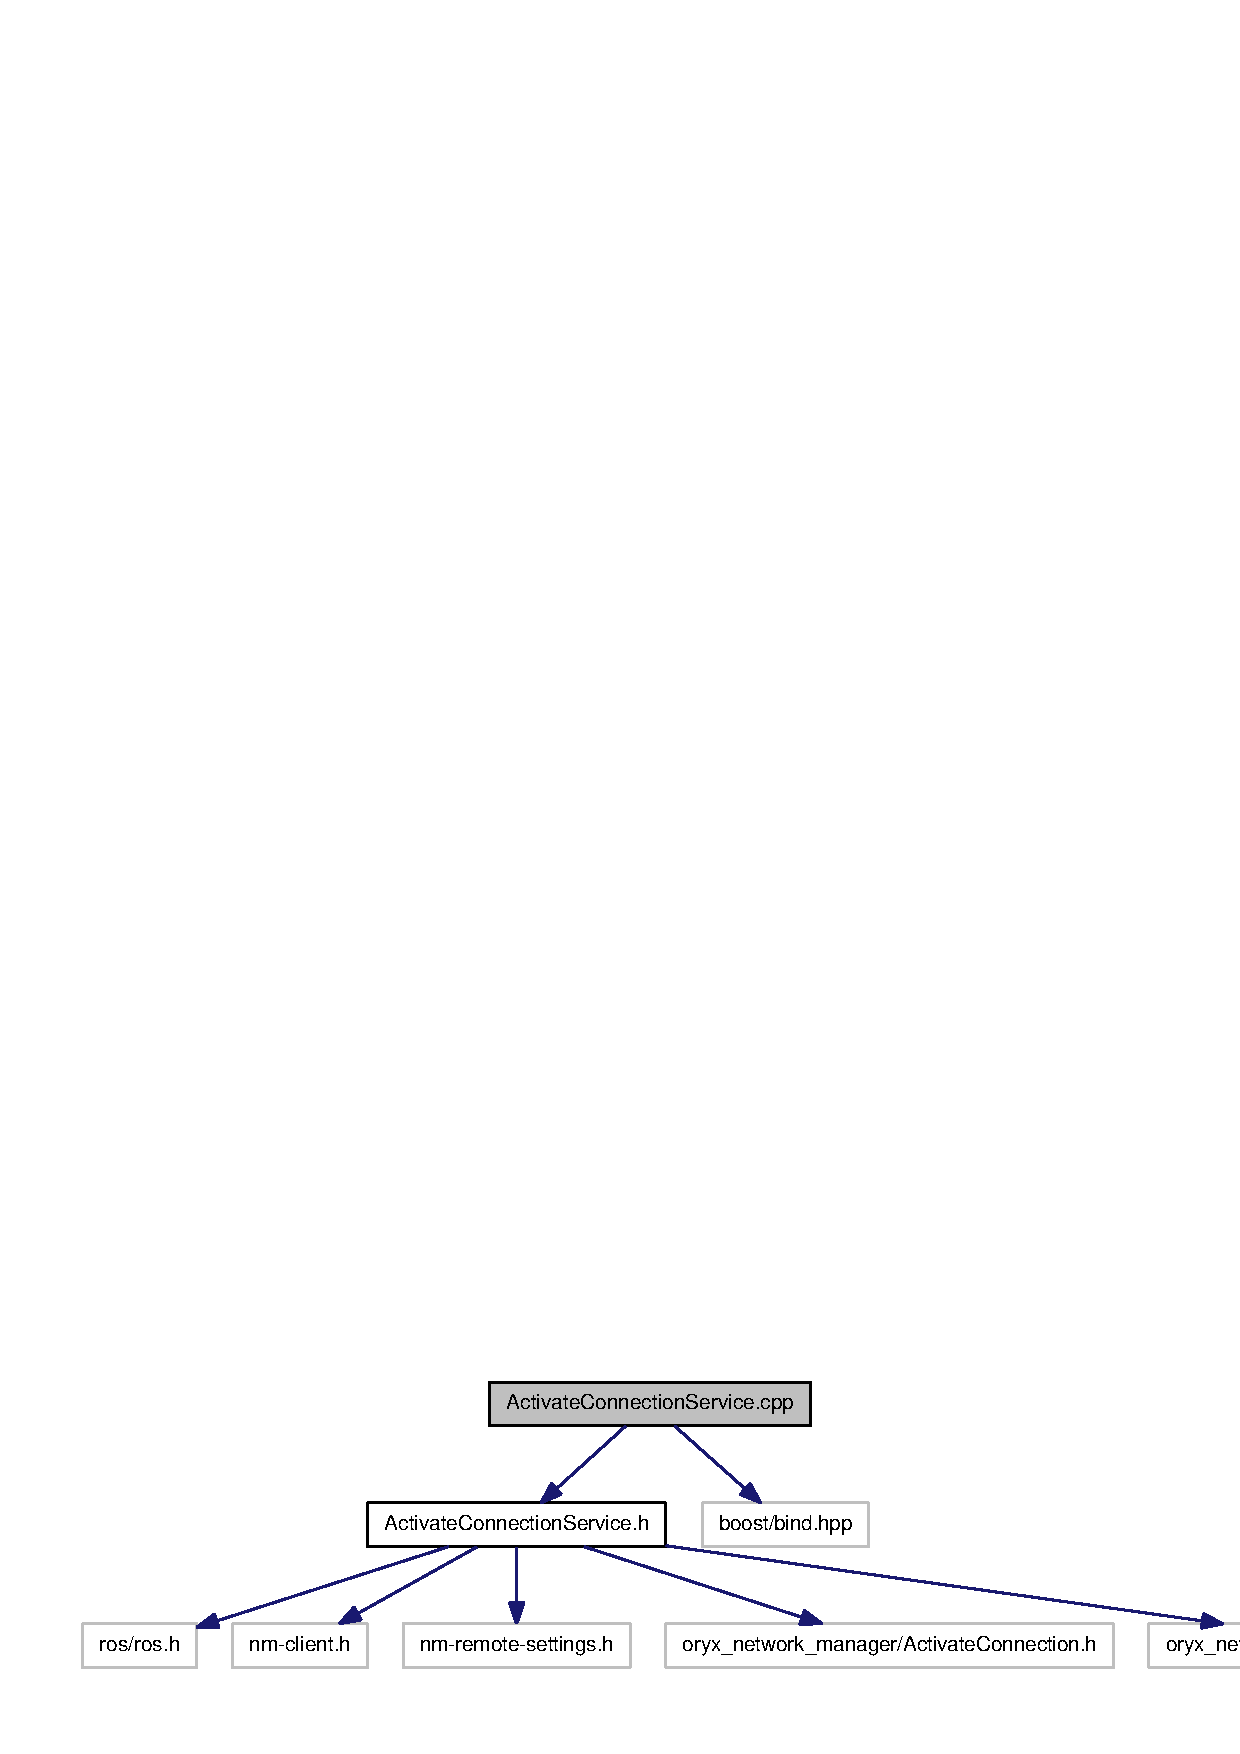
\includegraphics[width=350pt]{ActivateConnectionService_8cpp__incl}
\end{center}
\end{figure}

\section{\-Activate\-Connection\-Service.\-h \-File \-Reference}
\label{ActivateConnectionService_8h}\index{\-Activate\-Connection\-Service.\-h@{\-Activate\-Connection\-Service.\-h}}
{\ttfamily \#include \char`\"{}ros/ros.\-h\char`\"{}}\*
{\ttfamily \#include \char`\"{}nm-\/client.\-h\char`\"{}}\*
{\ttfamily \#include $<$nm-\/remote-\/settings.\-h$>$}\*
{\ttfamily \#include \char`\"{}oryx\-\_\-network\-\_\-manager/\-Activate\-Connection.\-h\char`\"{}}\*
{\ttfamily \#include \char`\"{}oryx\-\_\-network\-\_\-manager/\-Network\-Connections.\-h\char`\"{}}\*
\-Include dependency graph for \-Activate\-Connection\-Service.\-h\-:
\nopagebreak
\begin{figure}[H]
\begin{center}
\leavevmode
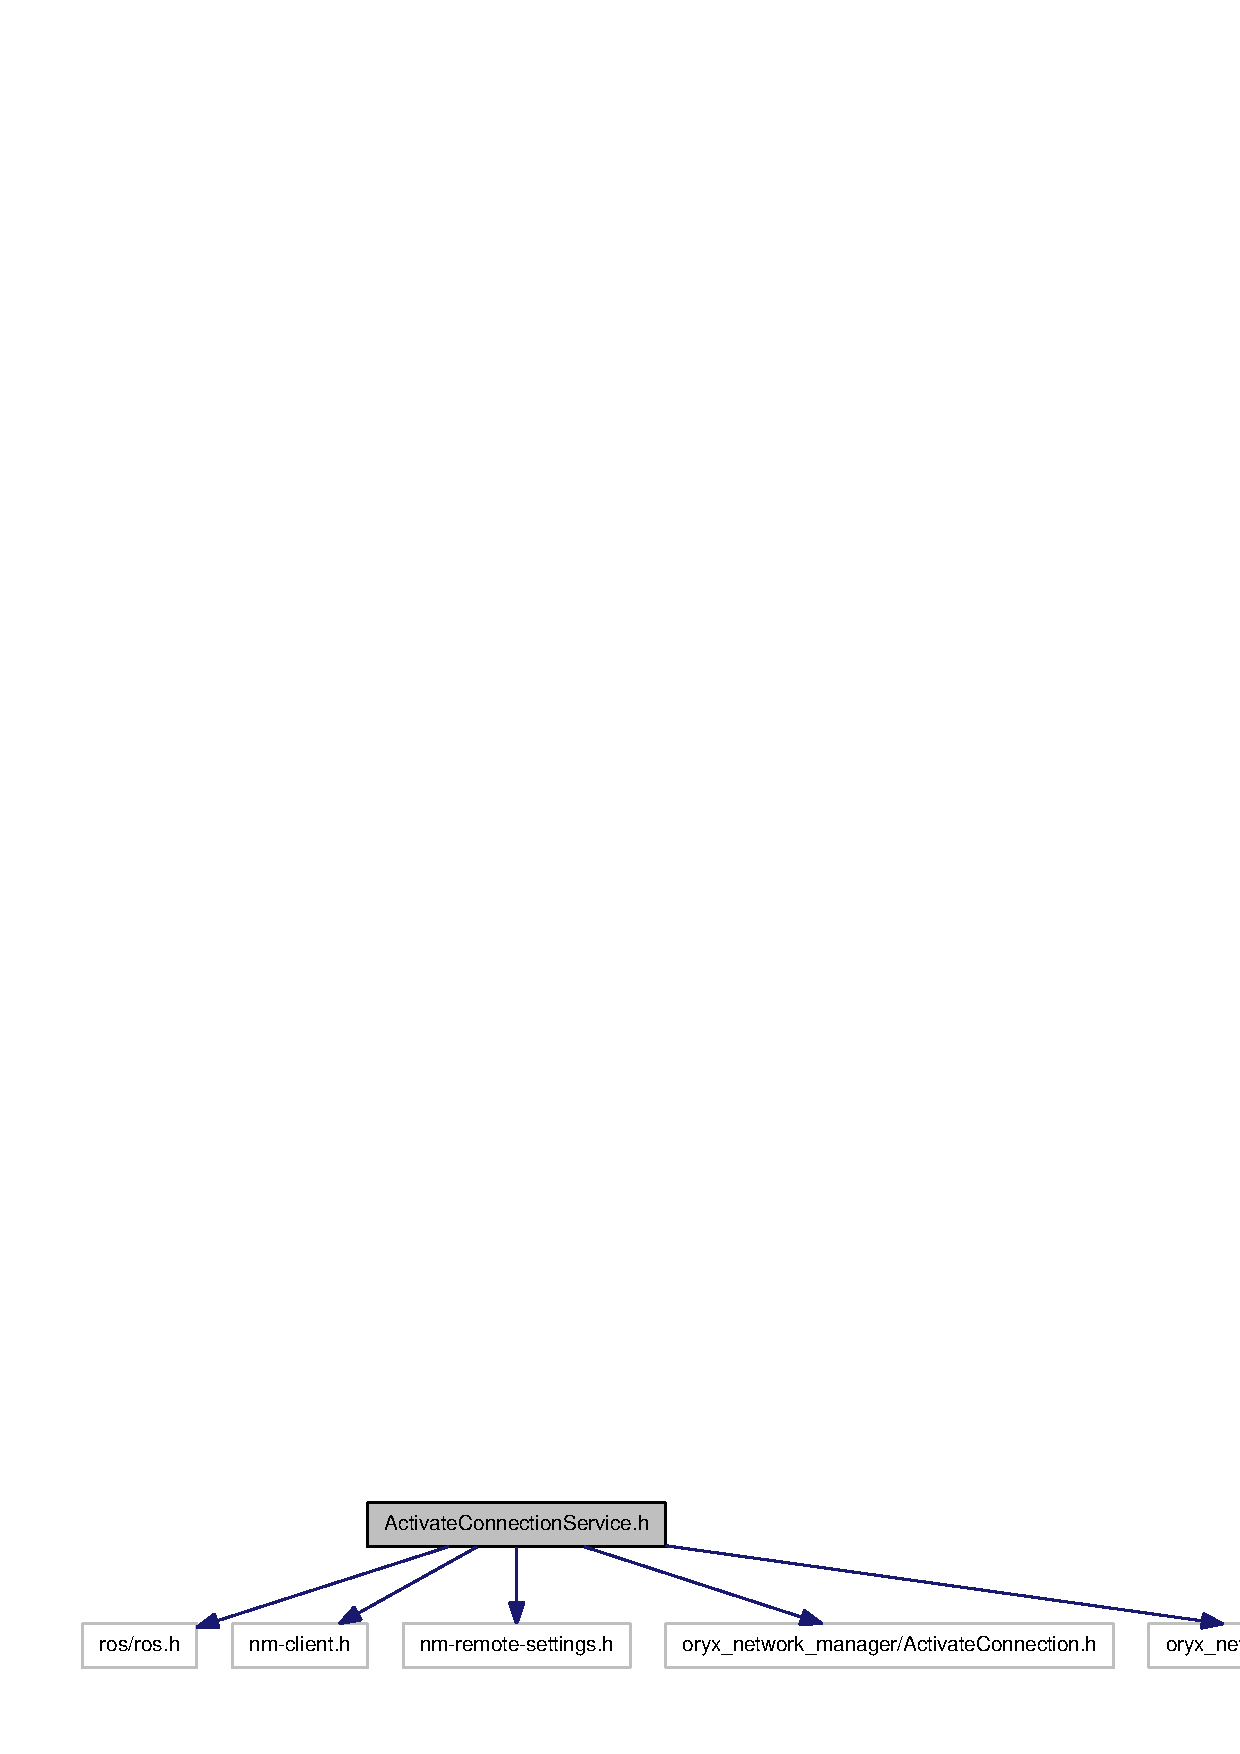
\includegraphics[width=350pt]{ActivateConnectionService_8h__incl}
\end{center}
\end{figure}
\-This graph shows which files directly or indirectly include this file\-:
\nopagebreak
\begin{figure}[H]
\begin{center}
\leavevmode
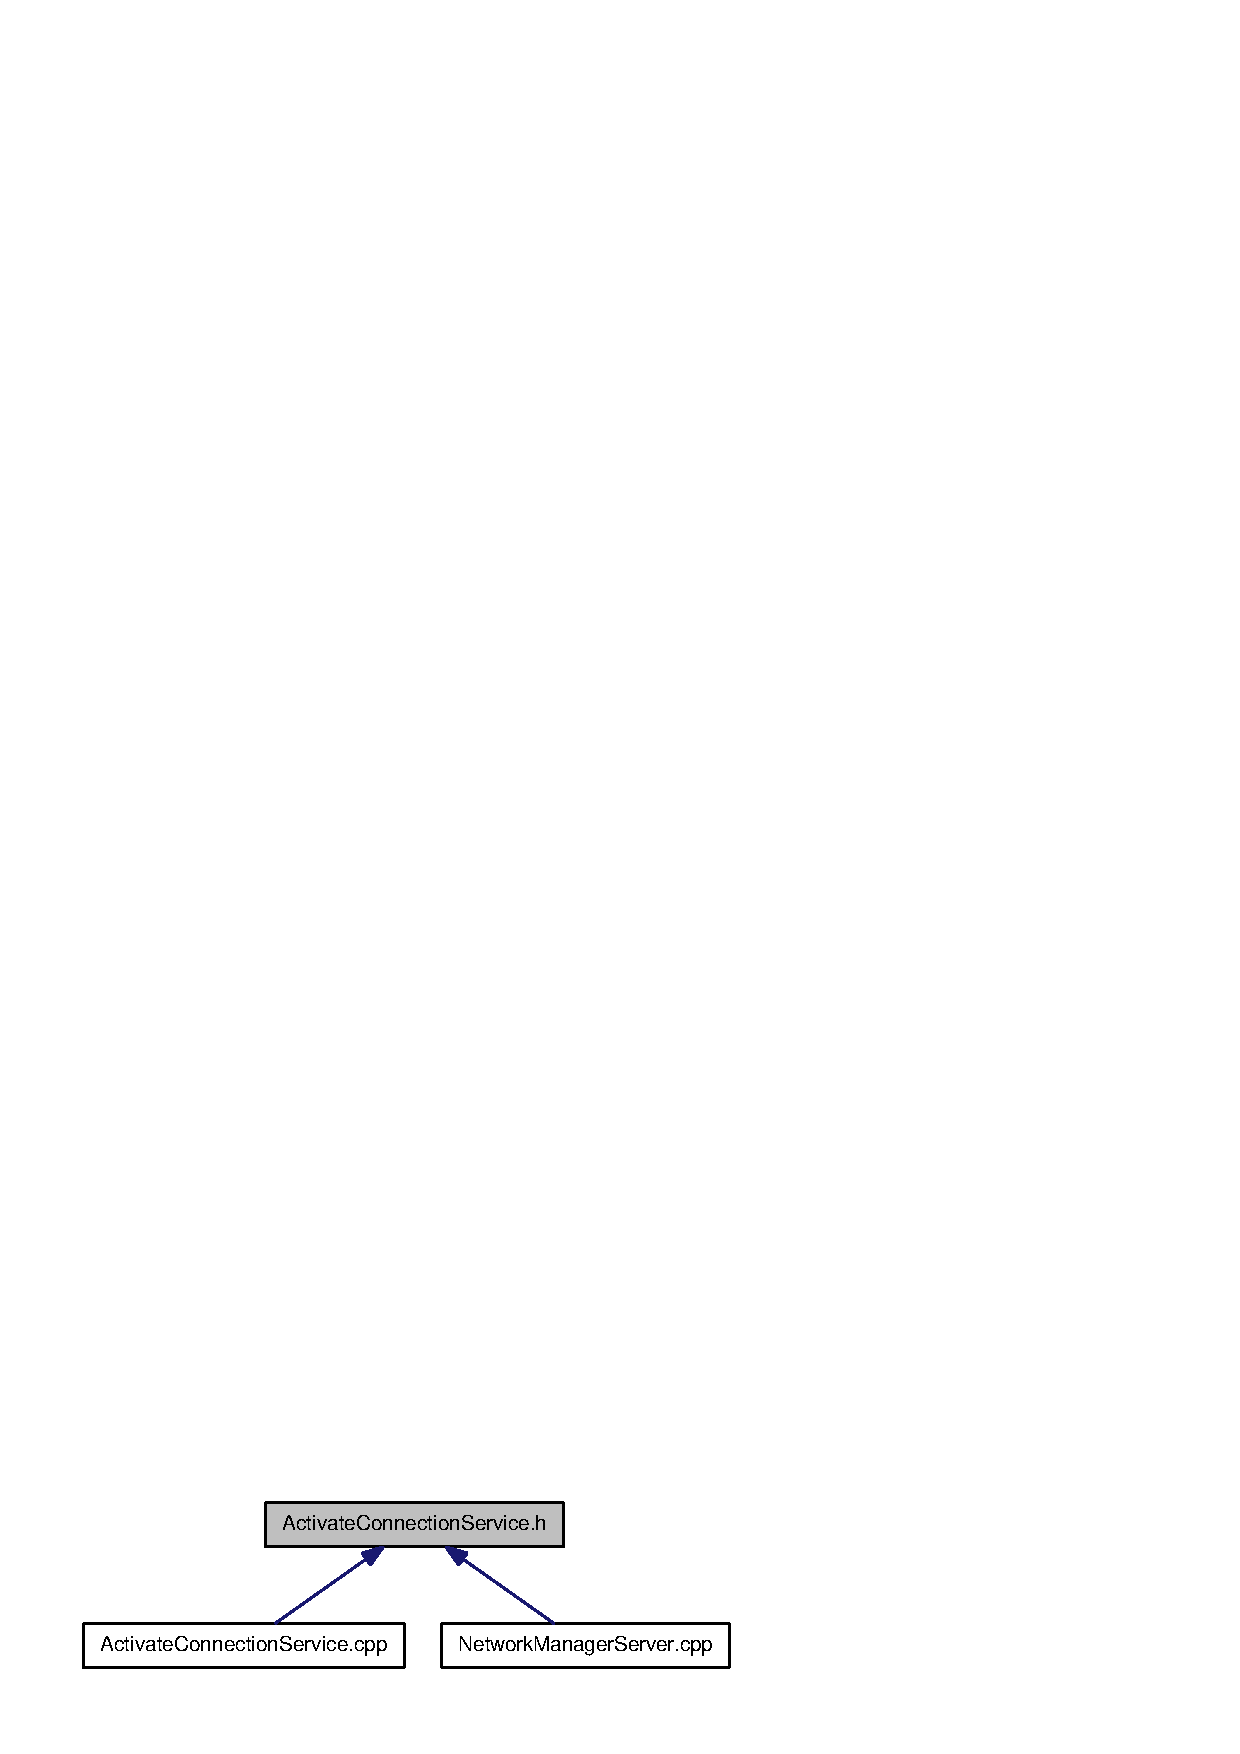
\includegraphics[width=350pt]{ActivateConnectionService_8h__dep__incl}
\end{center}
\end{figure}
\subsection*{\-Classes}
\begin{DoxyCompactItemize}
\item 
class {\bf \-Activate\-Connection\-Service}
\end{DoxyCompactItemize}

\section{\-Active\-Network\-Connection\-Manager.\-cpp \-File \-Reference}
\label{ActiveNetworkConnectionManager_8cpp}\index{\-Active\-Network\-Connection\-Manager.\-cpp@{\-Active\-Network\-Connection\-Manager.\-cpp}}
{\ttfamily \#include \char`\"{}\-Active\-Network\-Connection\-Manager.\-h\char`\"{}}\*
{\ttfamily \#include $<$boost/bind.\-hpp$>$}\*
{\ttfamily \#include \char`\"{}\-Message\-Util.\-h\char`\"{}}\*
\-Include dependency graph for \-Active\-Network\-Connection\-Manager.\-cpp\-:
\nopagebreak
\begin{figure}[H]
\begin{center}
\leavevmode
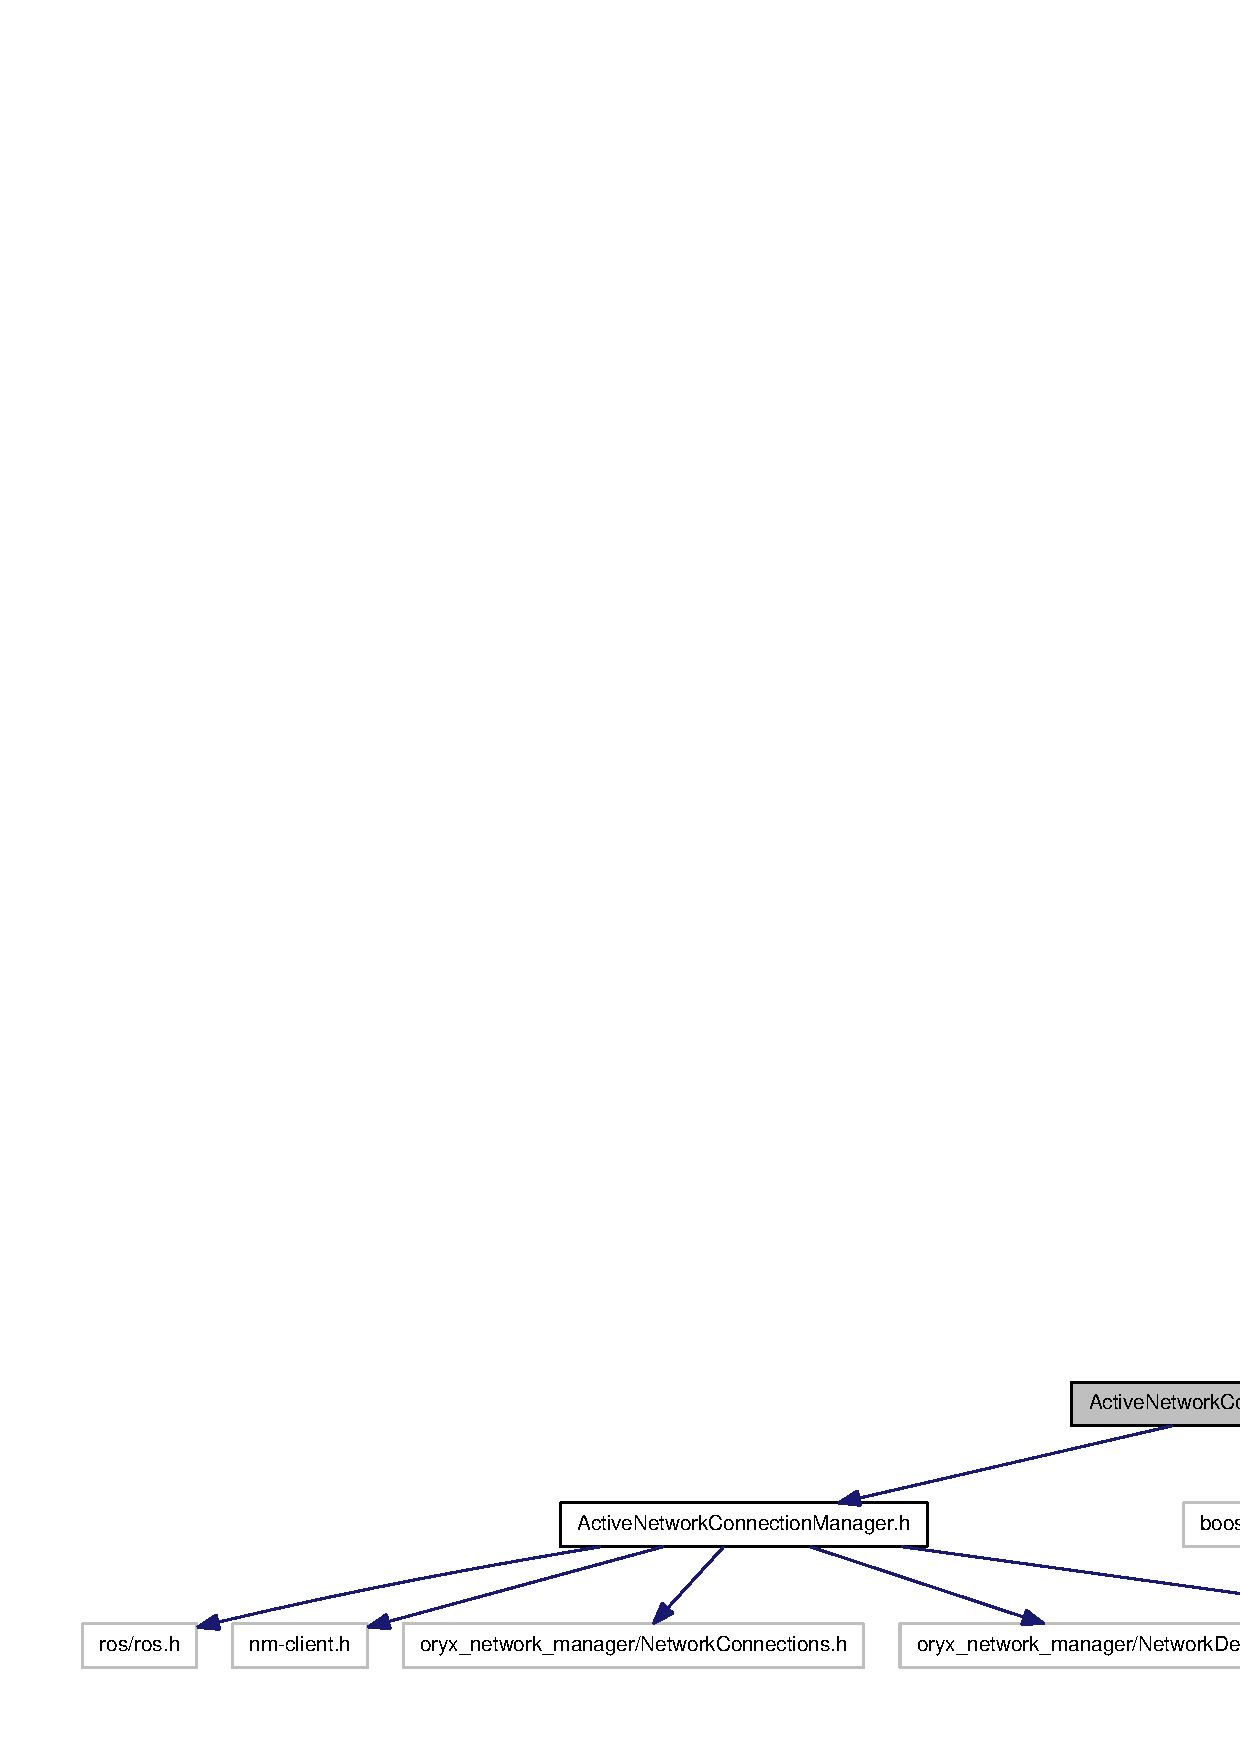
\includegraphics[width=350pt]{ActiveNetworkConnectionManager_8cpp__incl}
\end{center}
\end{figure}

\section{\-Active\-Network\-Connection\-Manager.\-h \-File \-Reference}
\label{ActiveNetworkConnectionManager_8h}\index{\-Active\-Network\-Connection\-Manager.\-h@{\-Active\-Network\-Connection\-Manager.\-h}}
{\ttfamily \#include \char`\"{}ros/ros.\-h\char`\"{}}\*
{\ttfamily \#include $<$nm-\/client.\-h$>$}\*
{\ttfamily \#include \char`\"{}oryx\-\_\-network\-\_\-manager/\-Network\-Connections.\-h\char`\"{}}\*
{\ttfamily \#include \char`\"{}oryx\-\_\-network\-\_\-manager/\-Network\-Devices.\-h\char`\"{}}\*
{\ttfamily \#include \char`\"{}oryx\-\_\-network\-\_\-manager/\-Active\-Network\-Connections.\-h\char`\"{}}\*
\-Include dependency graph for \-Active\-Network\-Connection\-Manager.\-h\-:
\nopagebreak
\begin{figure}[H]
\begin{center}
\leavevmode
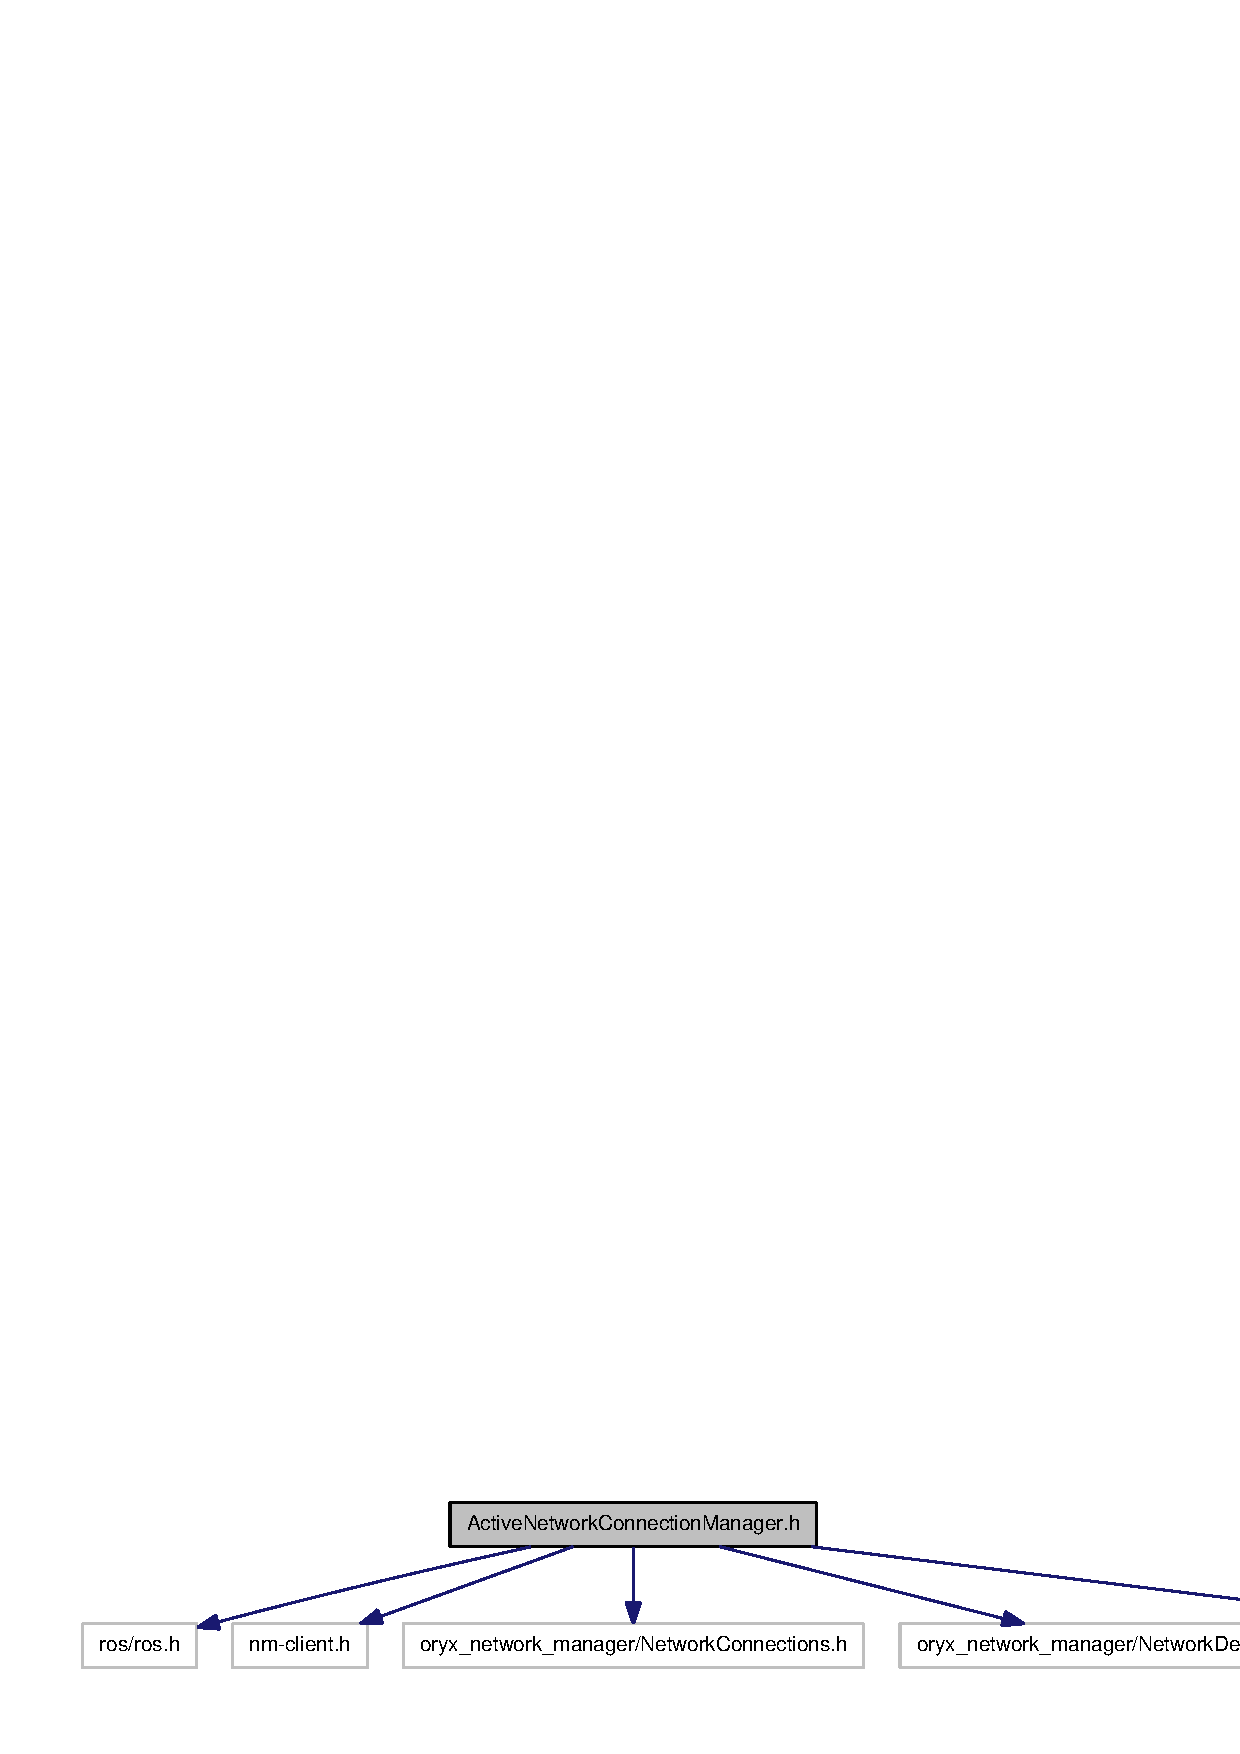
\includegraphics[width=350pt]{ActiveNetworkConnectionManager_8h__incl}
\end{center}
\end{figure}
\-This graph shows which files directly or indirectly include this file\-:
\nopagebreak
\begin{figure}[H]
\begin{center}
\leavevmode
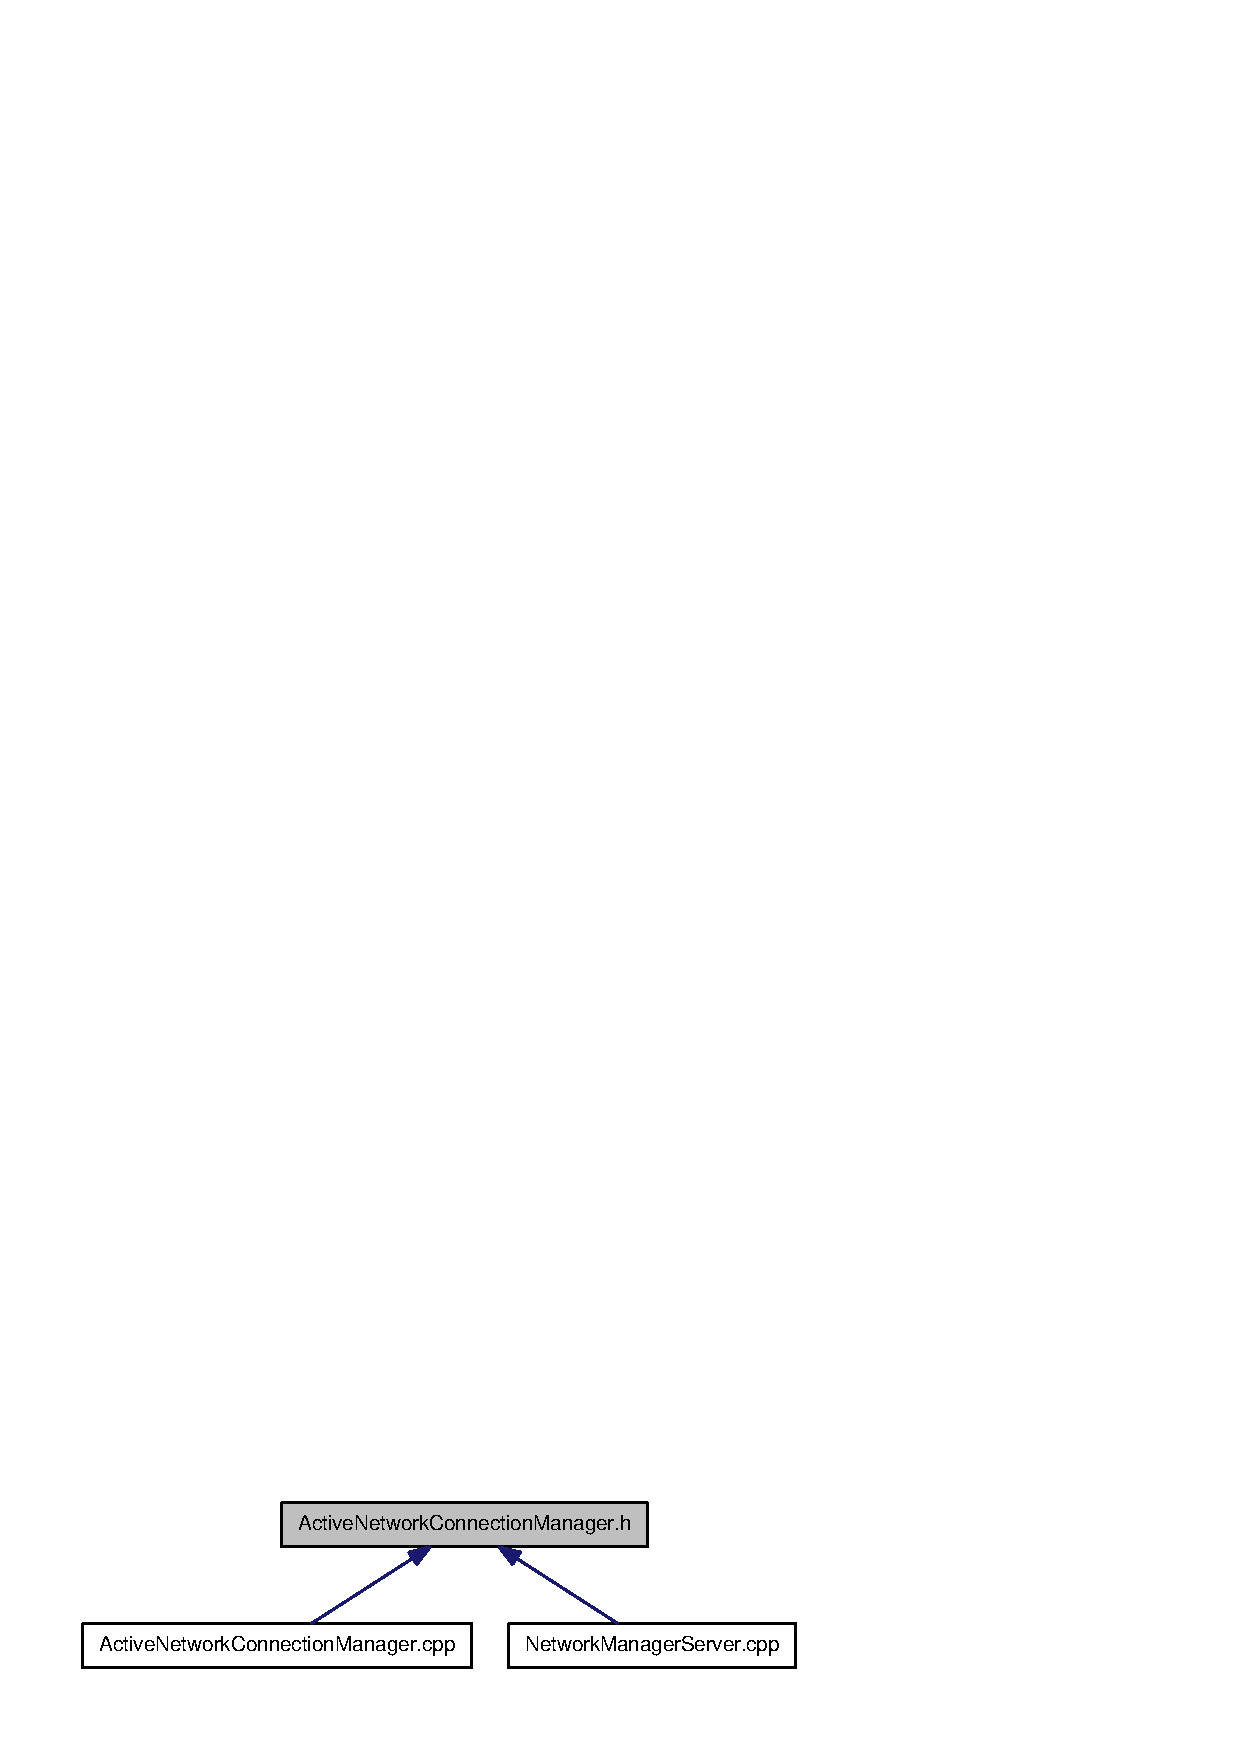
\includegraphics[width=350pt]{ActiveNetworkConnectionManager_8h__dep__incl}
\end{center}
\end{figure}
\subsection*{\-Classes}
\begin{DoxyCompactItemize}
\item 
class {\bf \-Active\-Network\-Connection\-Manager}
\end{DoxyCompactItemize}

\section{mainpage.\-dox \-File \-Reference}
\label{mainpage_8dox}\index{mainpage.\-dox@{mainpage.\-dox}}

\section{\-Message\-Util.\-h \-File \-Reference}
\label{MessageUtil_8h}\index{\-Message\-Util.\-h@{\-Message\-Util.\-h}}
{\ttfamily \#include \char`\"{}std\-\_\-msgs/\-Header.\-h\char`\"{}}\*
\-Include dependency graph for \-Message\-Util.\-h\-:
\nopagebreak
\begin{figure}[H]
\begin{center}
\leavevmode
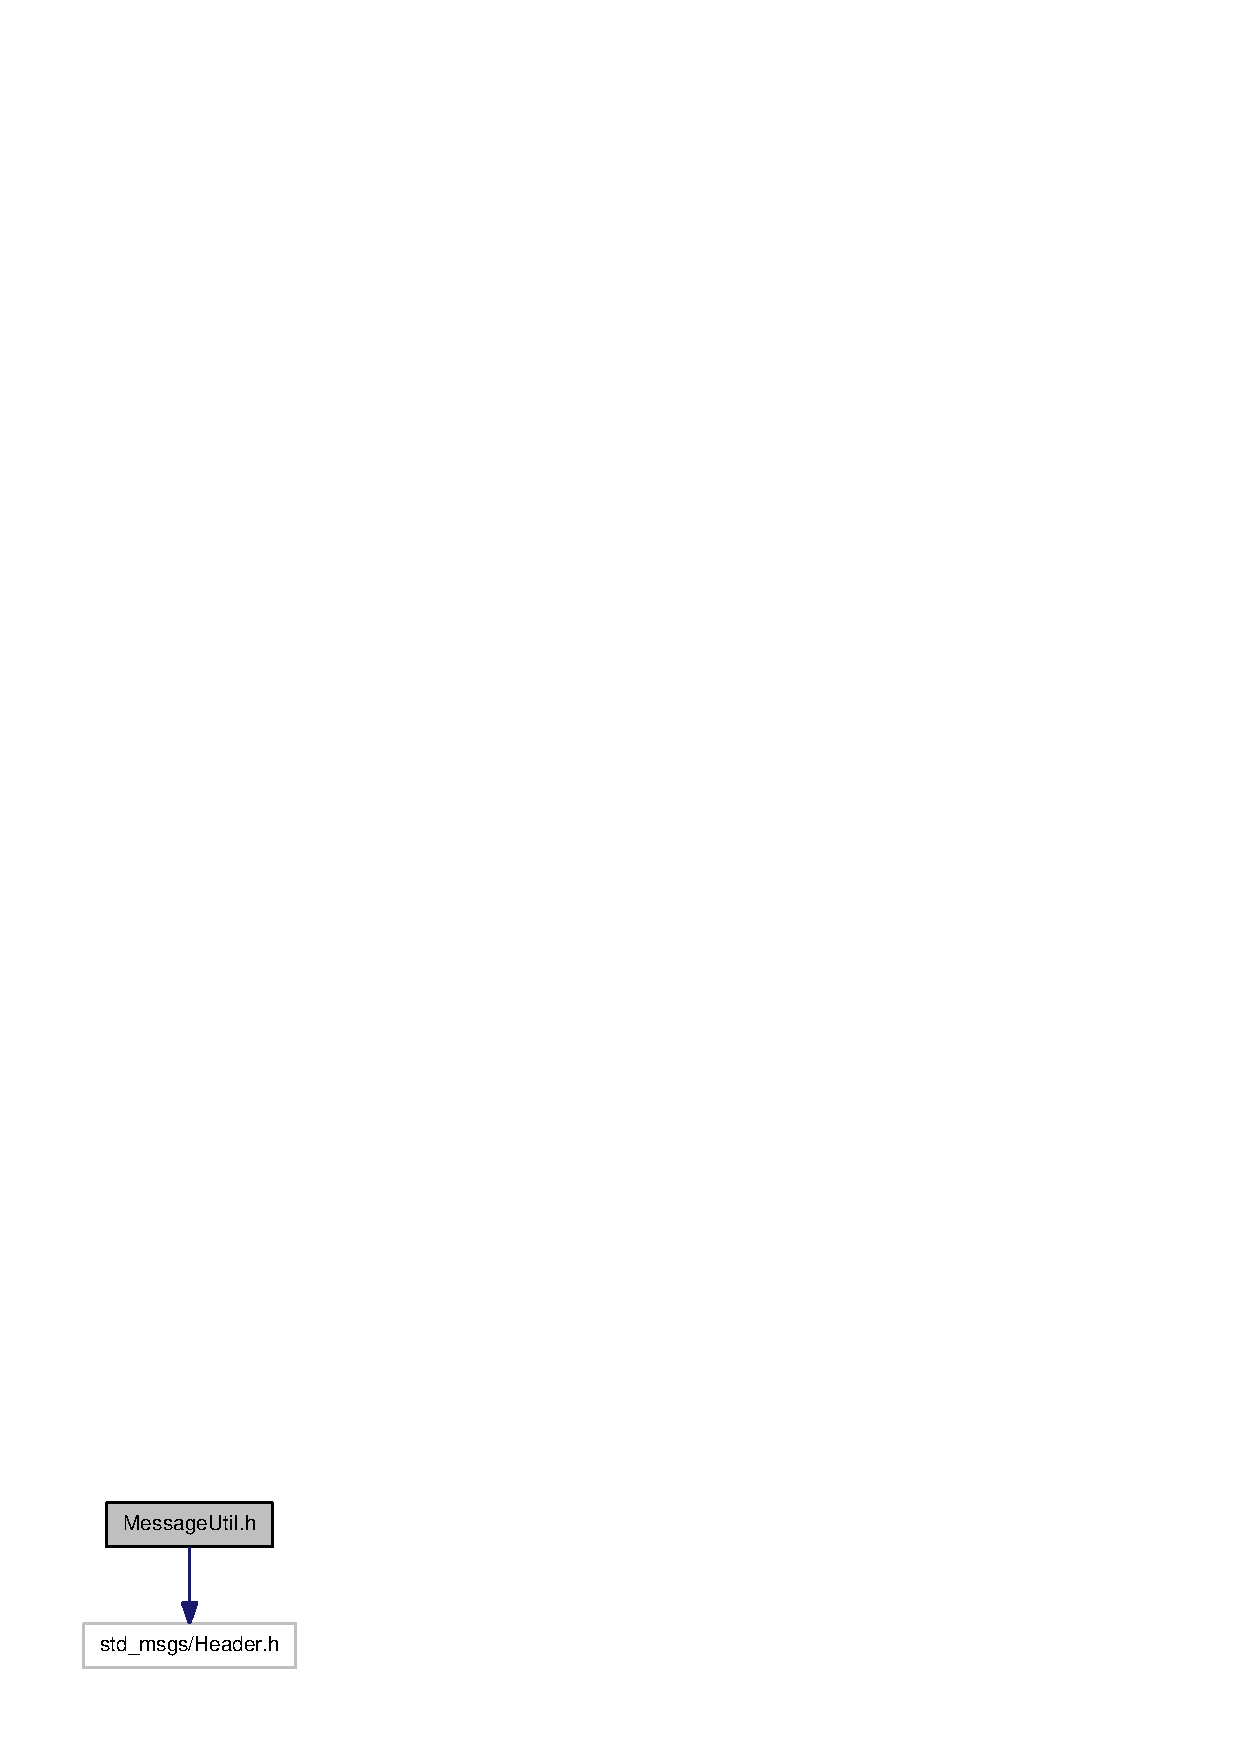
\includegraphics[width=146pt]{MessageUtil_8h__incl}
\end{center}
\end{figure}
\-This graph shows which files directly or indirectly include this file\-:
\nopagebreak
\begin{figure}[H]
\begin{center}
\leavevmode
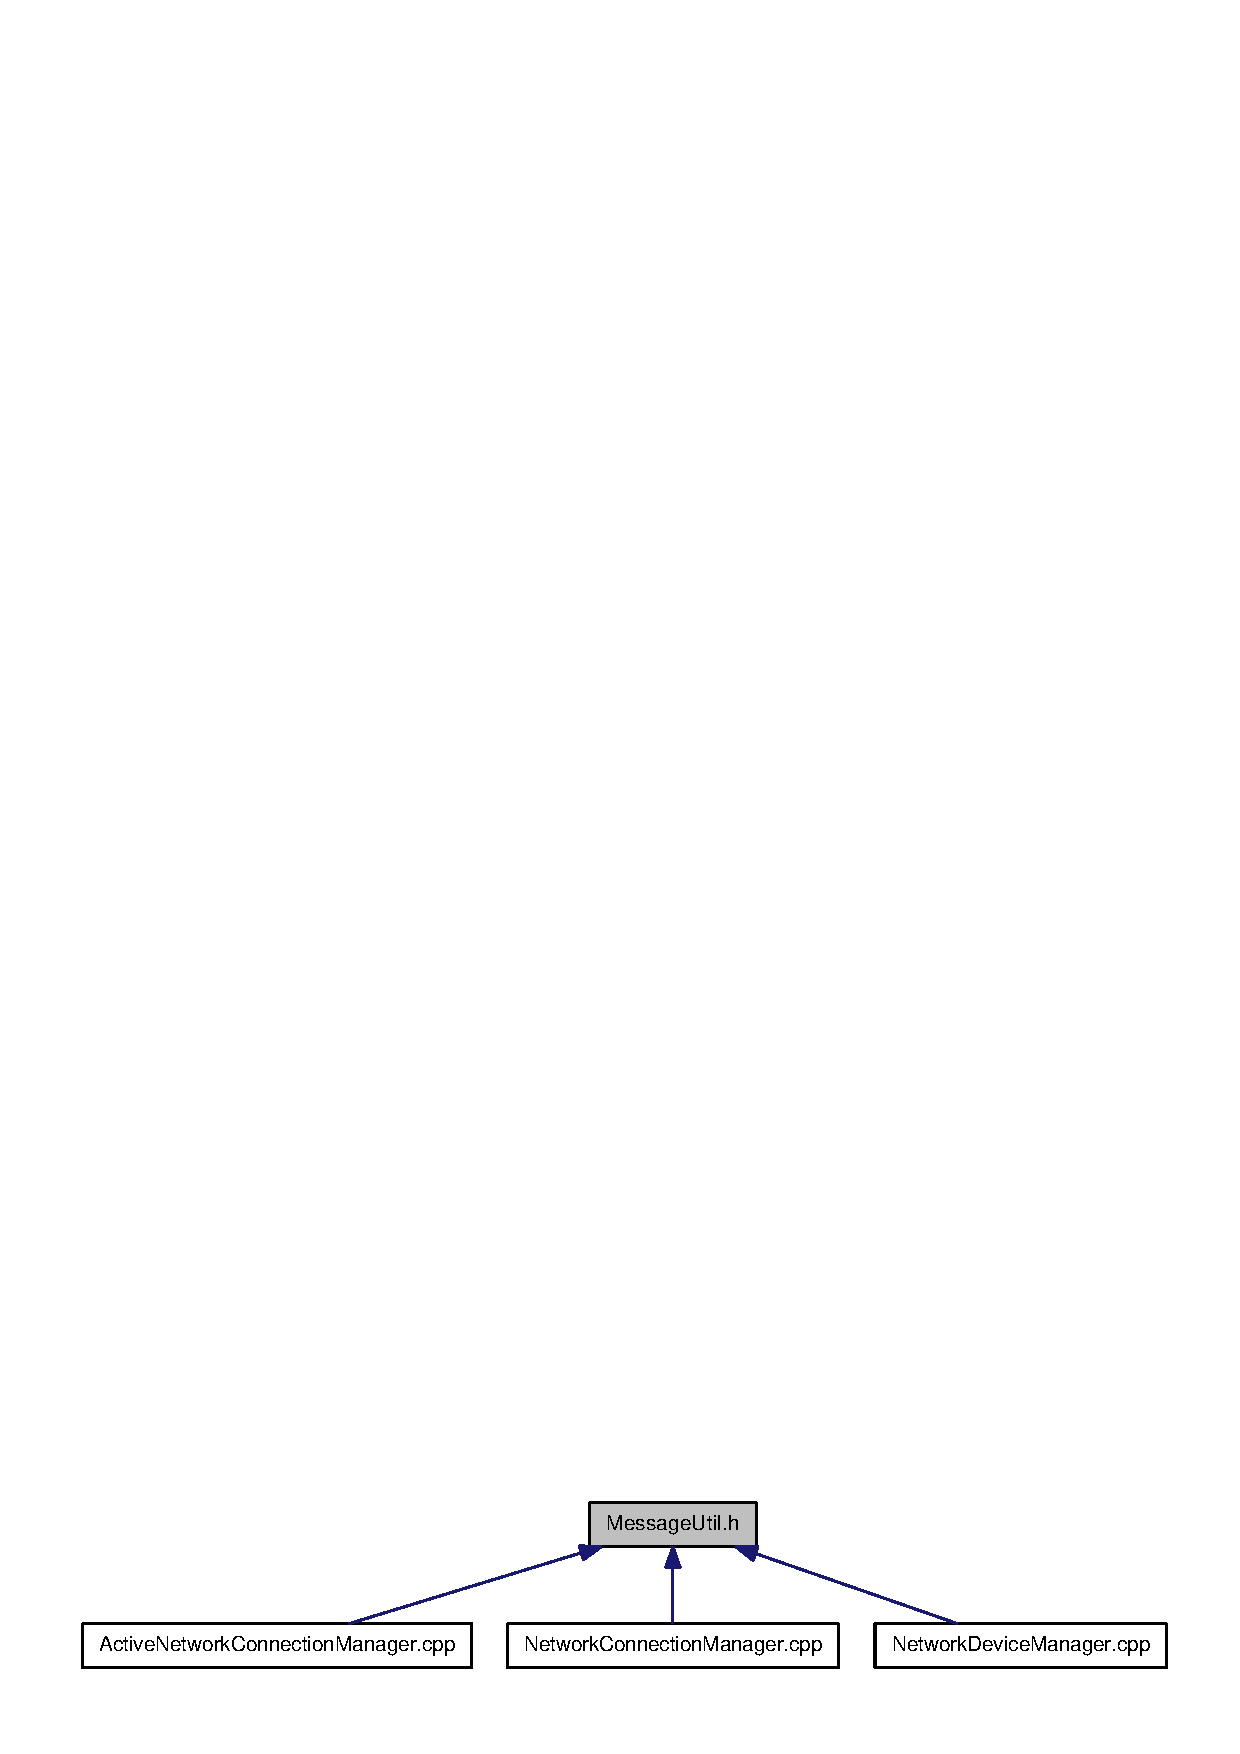
\includegraphics[width=350pt]{MessageUtil_8h__dep__incl}
\end{center}
\end{figure}
\subsection*{\-Functions}
\begin{DoxyCompactItemize}
\item 
static void {\bf fill\-\_\-header\-\_\-message} (std\-\_\-msgs\-::\-Header \&header, uint32\-\_\-t seq)
\end{DoxyCompactItemize}


\subsection{\-Function \-Documentation}
\index{\-Message\-Util.\-h@{\-Message\-Util.\-h}!fill\-\_\-header\-\_\-message@{fill\-\_\-header\-\_\-message}}
\index{fill\-\_\-header\-\_\-message@{fill\-\_\-header\-\_\-message}!MessageUtil.h@{\-Message\-Util.\-h}}
\subsubsection[{fill\-\_\-header\-\_\-message}]{\setlength{\rightskip}{0pt plus 5cm}static void {\bf fill\-\_\-header\-\_\-message} (
\begin{DoxyParamCaption}
\item[{std\-\_\-msgs\-::\-Header \&}]{header, }
\item[{uint32\-\_\-t}]{seq}
\end{DoxyParamCaption}
)\hspace{0.3cm}{\ttfamily  [inline, static]}}\label{MessageUtil_8h_adc2e74fa372c4b8d83da83124b4cf192}
fill in values in a \-R\-O\-S header message 

\-Definition at line 16 of file \-Message\-Util.\-h.


\section{\-Network\-Configuration\-Manager.\-cpp \-File \-Reference}
\label{NetworkConfigurationManager_8cpp}\index{\-Network\-Configuration\-Manager.\-cpp@{\-Network\-Configuration\-Manager.\-cpp}}
{\ttfamily \#include \char`\"{}\-Network\-Configuration\-Manager.\-h\char`\"{}}\*
{\ttfamily \#include $<$stdio.\-h$>$}\*
\-Include dependency graph for \-Network\-Configuration\-Manager.\-cpp\-:
\nopagebreak
\begin{figure}[H]
\begin{center}
\leavevmode
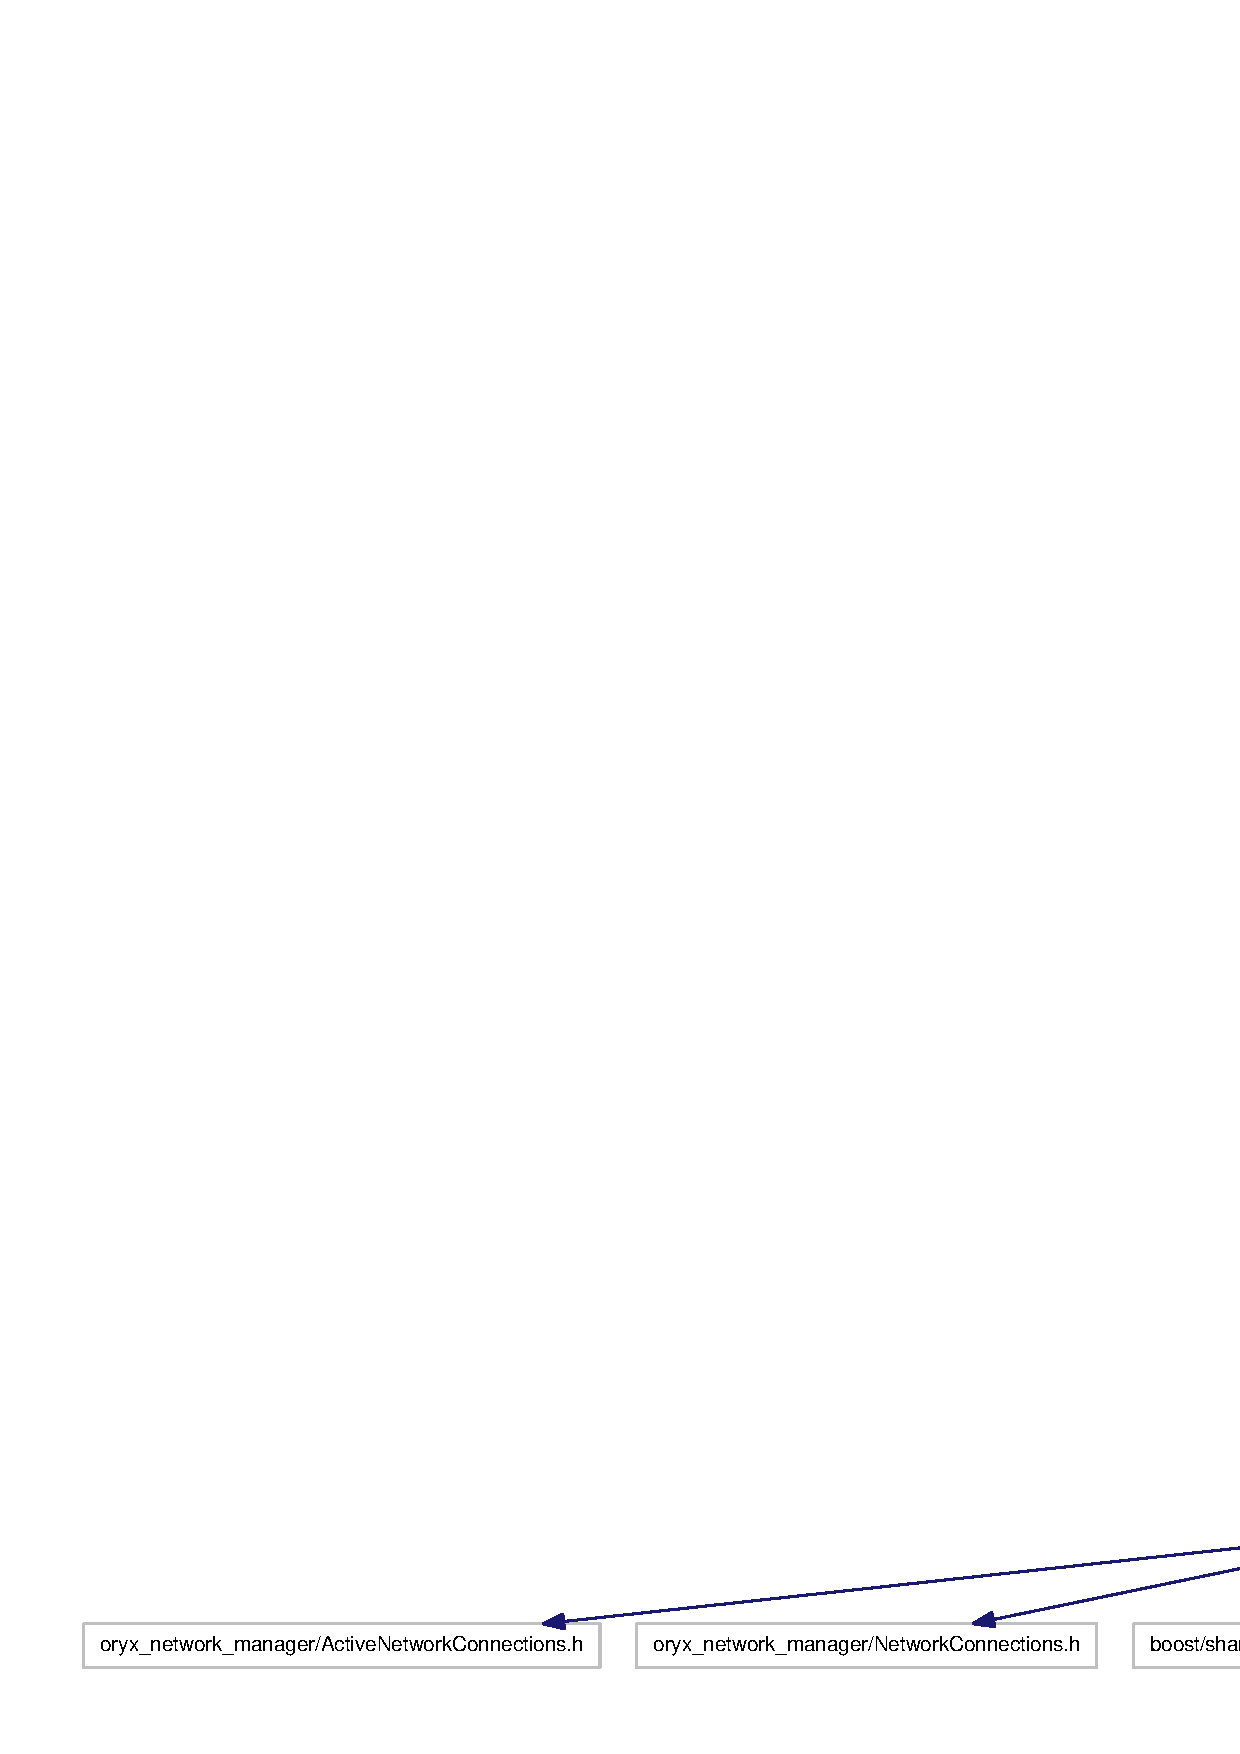
\includegraphics[width=350pt]{NetworkConfigurationManager_8cpp__incl}
\end{center}
\end{figure}

\section{\-Network\-Configuration\-Manager.\-h \-File \-Reference}
\label{NetworkConfigurationManager_8h}\index{\-Network\-Configuration\-Manager.\-h@{\-Network\-Configuration\-Manager.\-h}}
{\ttfamily \#include \char`\"{}oryx\-\_\-network\-\_\-manager/\-Active\-Network\-Connections.\-h\char`\"{}}\*
{\ttfamily \#include \char`\"{}oryx\-\_\-network\-\_\-manager/\-Network\-Connections.\-h\char`\"{}}\*
{\ttfamily \#include \char`\"{}boost/shared\-\_\-ptr.\-hpp\char`\"{}}\*
{\ttfamily \#include \char`\"{}ros/ros.\-h\char`\"{}}\*
{\ttfamily \#include $<$nm-\/client.\-h$>$}\*
{\ttfamily \#include $<$nm-\/remote-\/settings.\-h$>$}\*
{\ttfamily \#include $<$vector$>$}\*
\-Include dependency graph for \-Network\-Configuration\-Manager.\-h\-:
\nopagebreak
\begin{figure}[H]
\begin{center}
\leavevmode
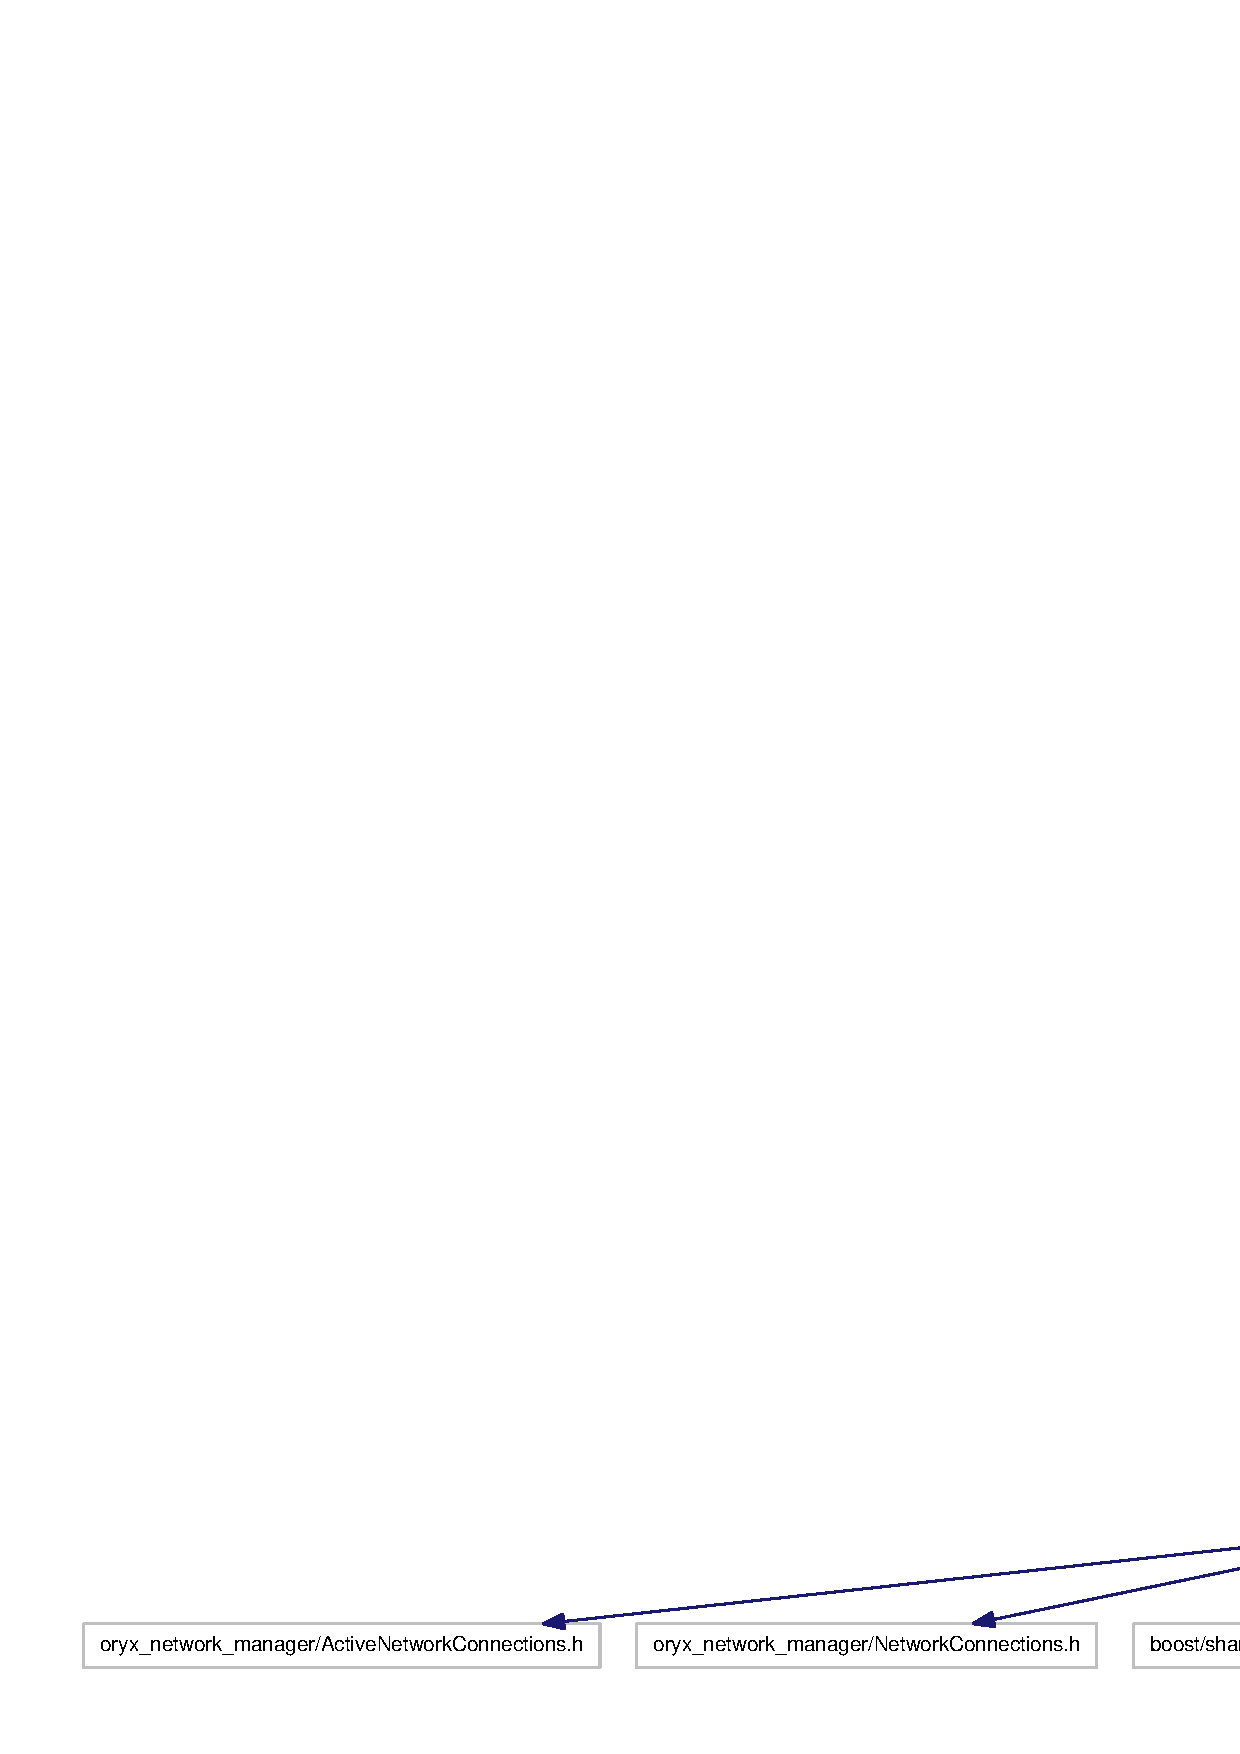
\includegraphics[width=350pt]{NetworkConfigurationManager_8h__incl}
\end{center}
\end{figure}
\-This graph shows which files directly or indirectly include this file\-:
\nopagebreak
\begin{figure}[H]
\begin{center}
\leavevmode
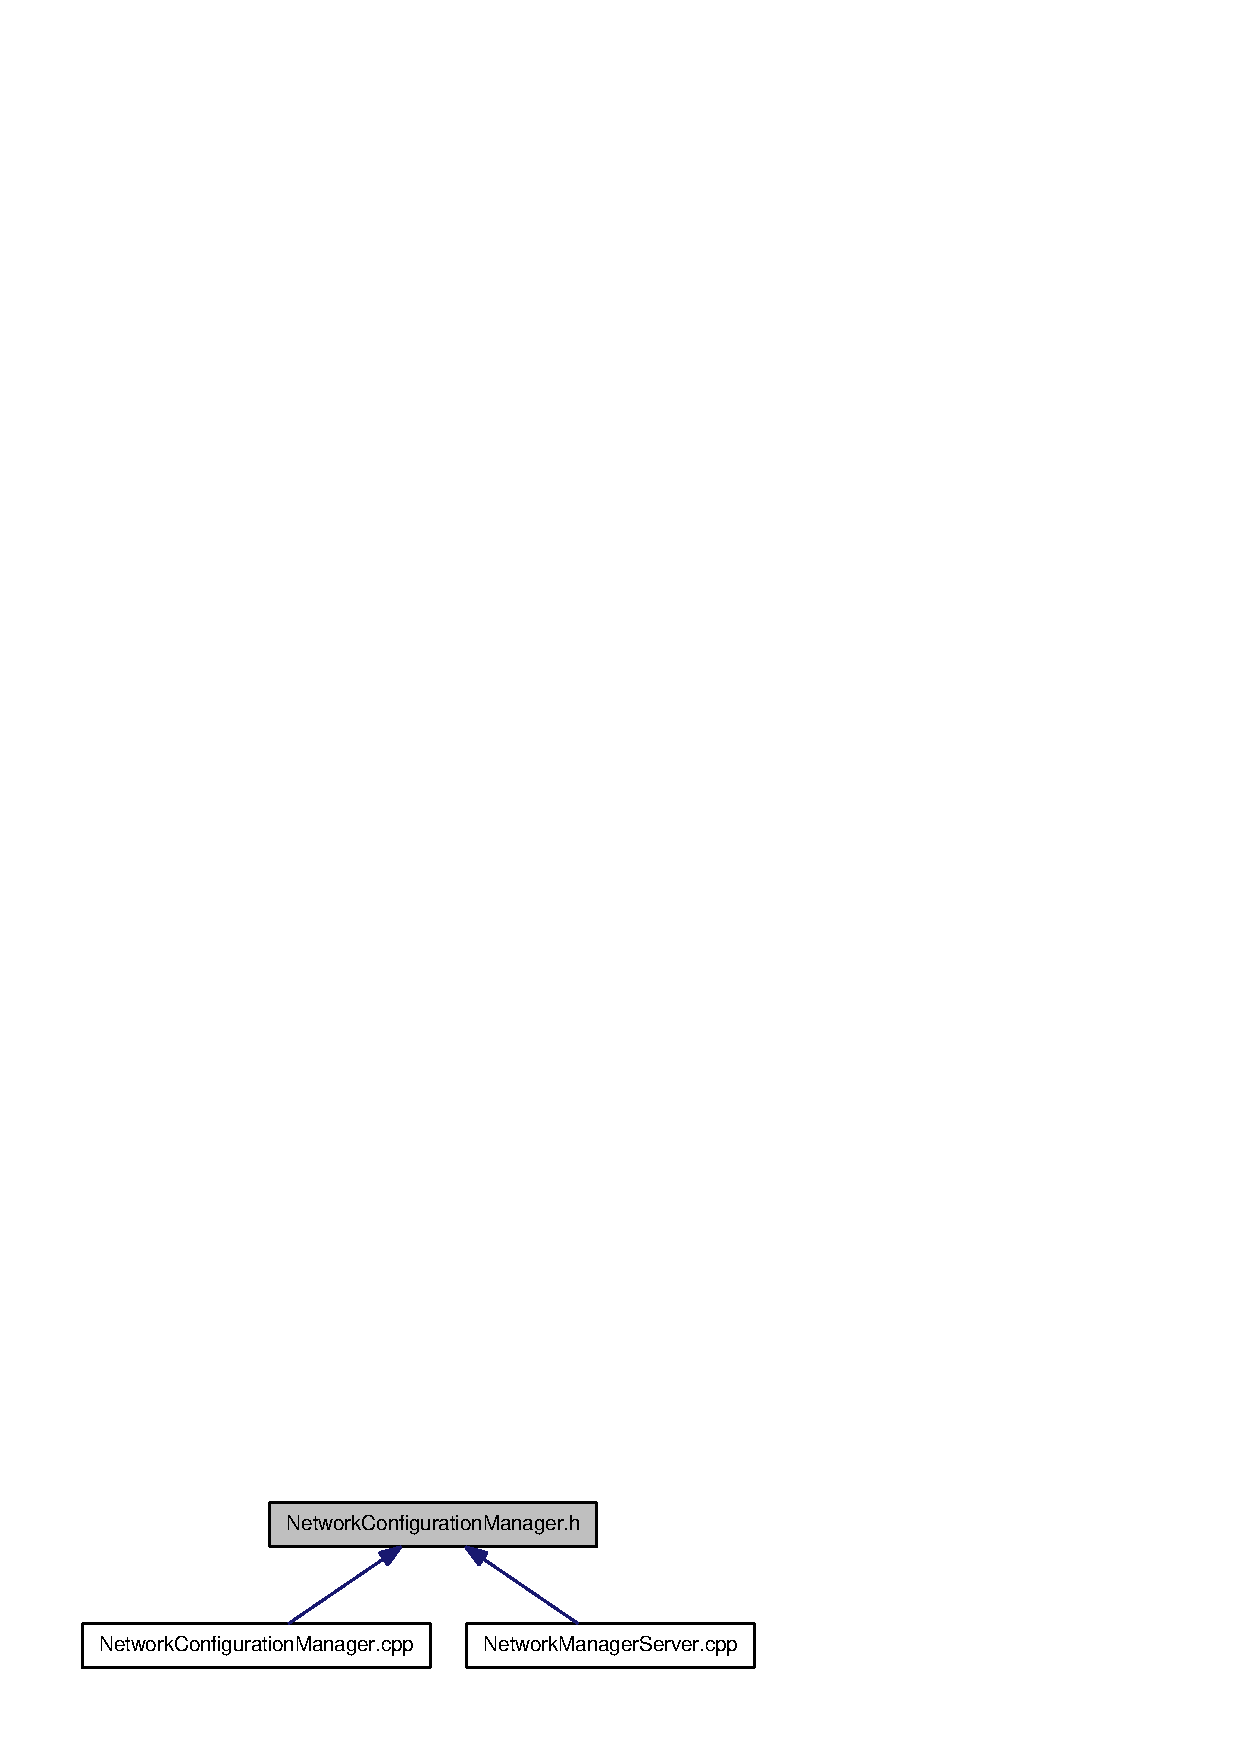
\includegraphics[width=350pt]{NetworkConfigurationManager_8h__dep__incl}
\end{center}
\end{figure}
\subsection*{\-Classes}
\begin{DoxyCompactItemize}
\item 
class {\bf \-Blank\-Network\-Config}
\item 
class {\bf \-Network\-Config}
\item 
class {\bf \-Network\-Configuration\-Manager}
\item 
class {\bf \-Network\-Connection\-Config}
\end{DoxyCompactItemize}

\section{\-Network\-Connection\-Manager.\-cpp \-File \-Reference}
\label{NetworkConnectionManager_8cpp}\index{\-Network\-Connection\-Manager.\-cpp@{\-Network\-Connection\-Manager.\-cpp}}
{\ttfamily \#include \char`\"{}\-Network\-Connection\-Manager.\-h\char`\"{}}\*
{\ttfamily \#include $<$nm-\/connection.\-h$>$}\*
{\ttfamily \#include $<$nm-\/setting-\/connection.\-h$>$}\*
{\ttfamily \#include $<$\-Network\-Manager.\-h$>$}\*
{\ttfamily \#include $<$nm-\/utils.\-h$>$}\*
{\ttfamily \#include \char`\"{}\-Message\-Util.\-h\char`\"{}}\*
\-Include dependency graph for \-Network\-Connection\-Manager.\-cpp\-:
\nopagebreak
\begin{figure}[H]
\begin{center}
\leavevmode
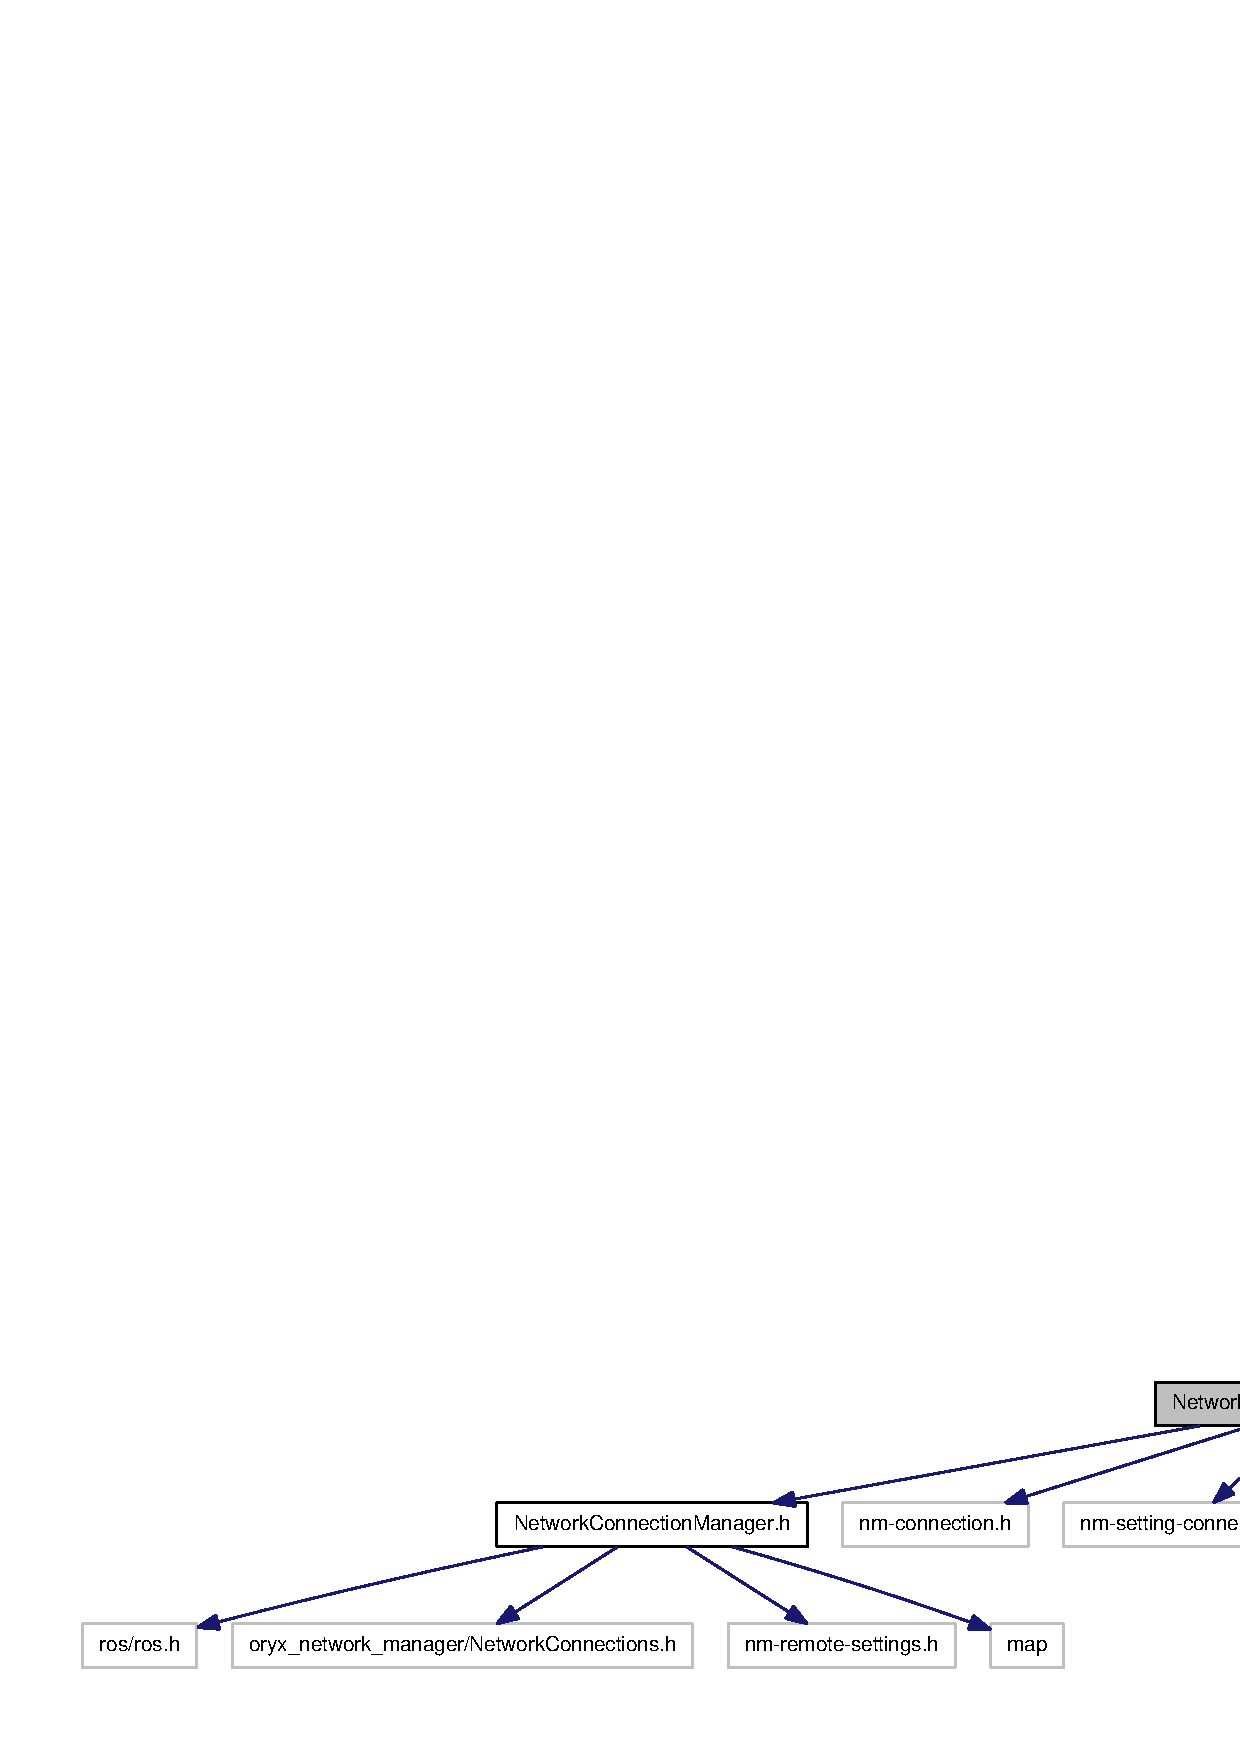
\includegraphics[width=350pt]{NetworkConnectionManager_8cpp__incl}
\end{center}
\end{figure}

\section{\-Network\-Connection\-Manager.\-h \-File \-Reference}
\label{NetworkConnectionManager_8h}\index{\-Network\-Connection\-Manager.\-h@{\-Network\-Connection\-Manager.\-h}}
{\ttfamily \#include \char`\"{}ros/ros.\-h\char`\"{}}\*
{\ttfamily \#include \char`\"{}oryx\-\_\-network\-\_\-manager/\-Network\-Connections.\-h\char`\"{}}\*
{\ttfamily \#include $<$nm-\/remote-\/settings.\-h$>$}\*
{\ttfamily \#include $<$map$>$}\*
\-Include dependency graph for \-Network\-Connection\-Manager.\-h\-:
\nopagebreak
\begin{figure}[H]
\begin{center}
\leavevmode
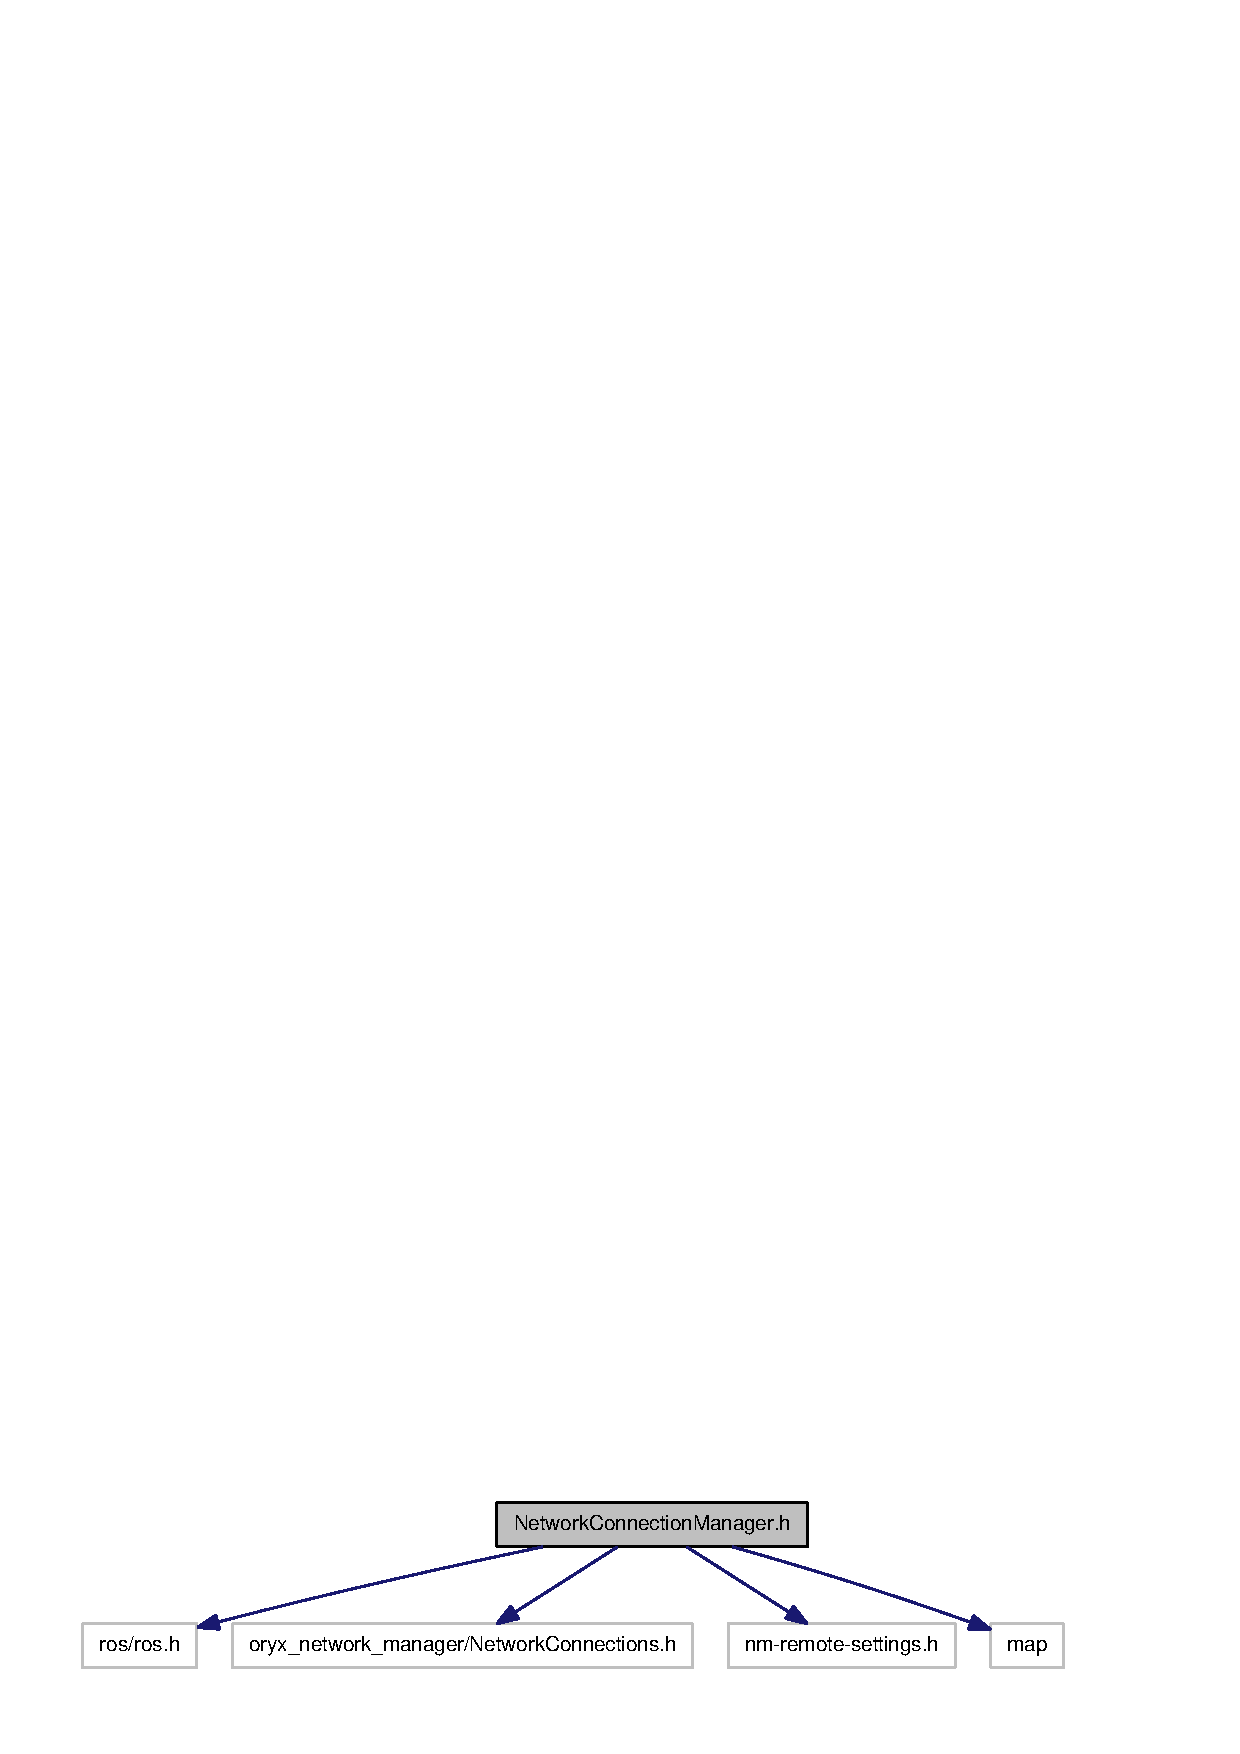
\includegraphics[width=350pt]{NetworkConnectionManager_8h__incl}
\end{center}
\end{figure}
\-This graph shows which files directly or indirectly include this file\-:
\nopagebreak
\begin{figure}[H]
\begin{center}
\leavevmode
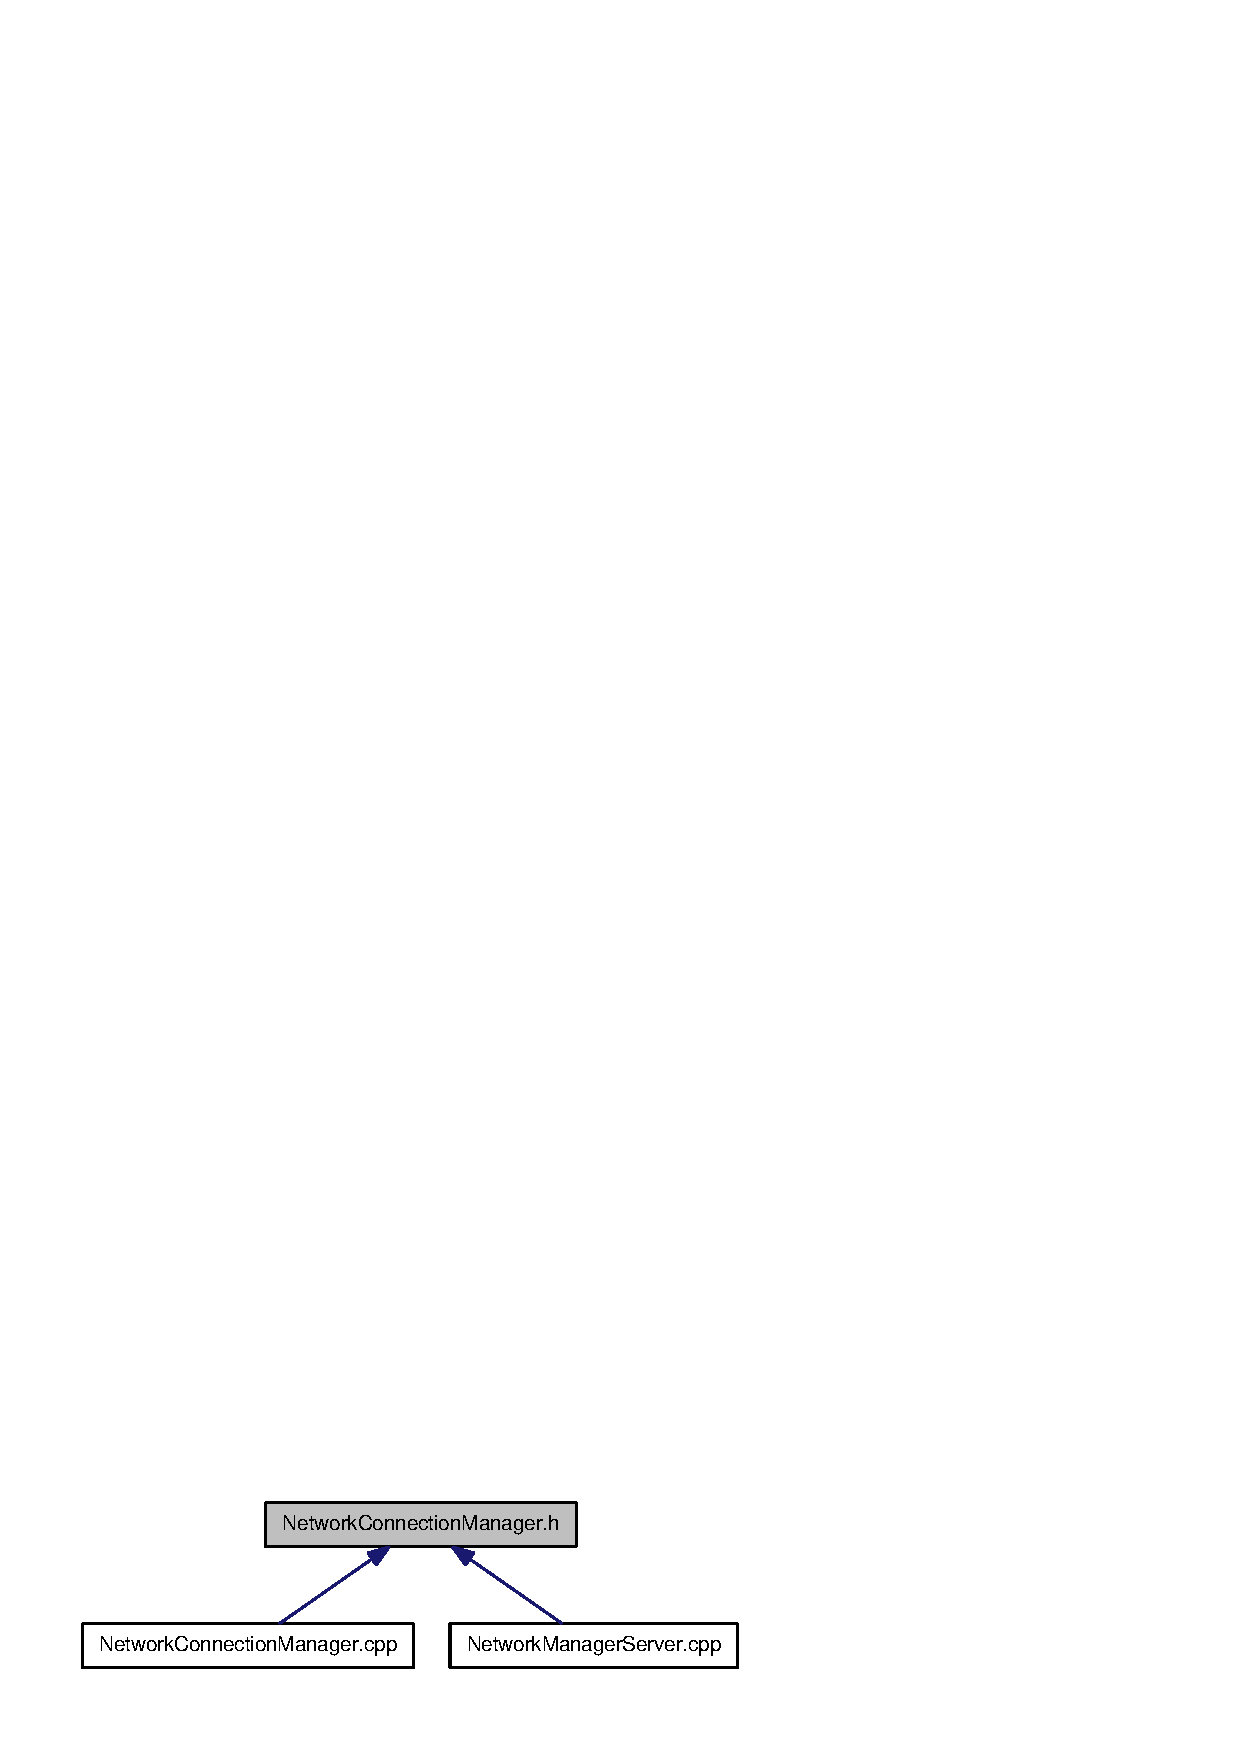
\includegraphics[width=350pt]{NetworkConnectionManager_8h__dep__incl}
\end{center}
\end{figure}
\subsection*{\-Classes}
\begin{DoxyCompactItemize}
\item 
class {\bf \-Network\-Connection\-Manager}
\end{DoxyCompactItemize}

\section{\-Network\-Device\-Manager.\-cpp \-File \-Reference}
\label{NetworkDeviceManager_8cpp}\index{\-Network\-Device\-Manager.\-cpp@{\-Network\-Device\-Manager.\-cpp}}
{\ttfamily \#include \char`\"{}\-Network\-Device\-Manager.\-h\char`\"{}}\*
{\ttfamily \#include \char`\"{}\-Message\-Util.\-h\char`\"{}}\*
\-Include dependency graph for \-Network\-Device\-Manager.\-cpp\-:
\nopagebreak
\begin{figure}[H]
\begin{center}
\leavevmode
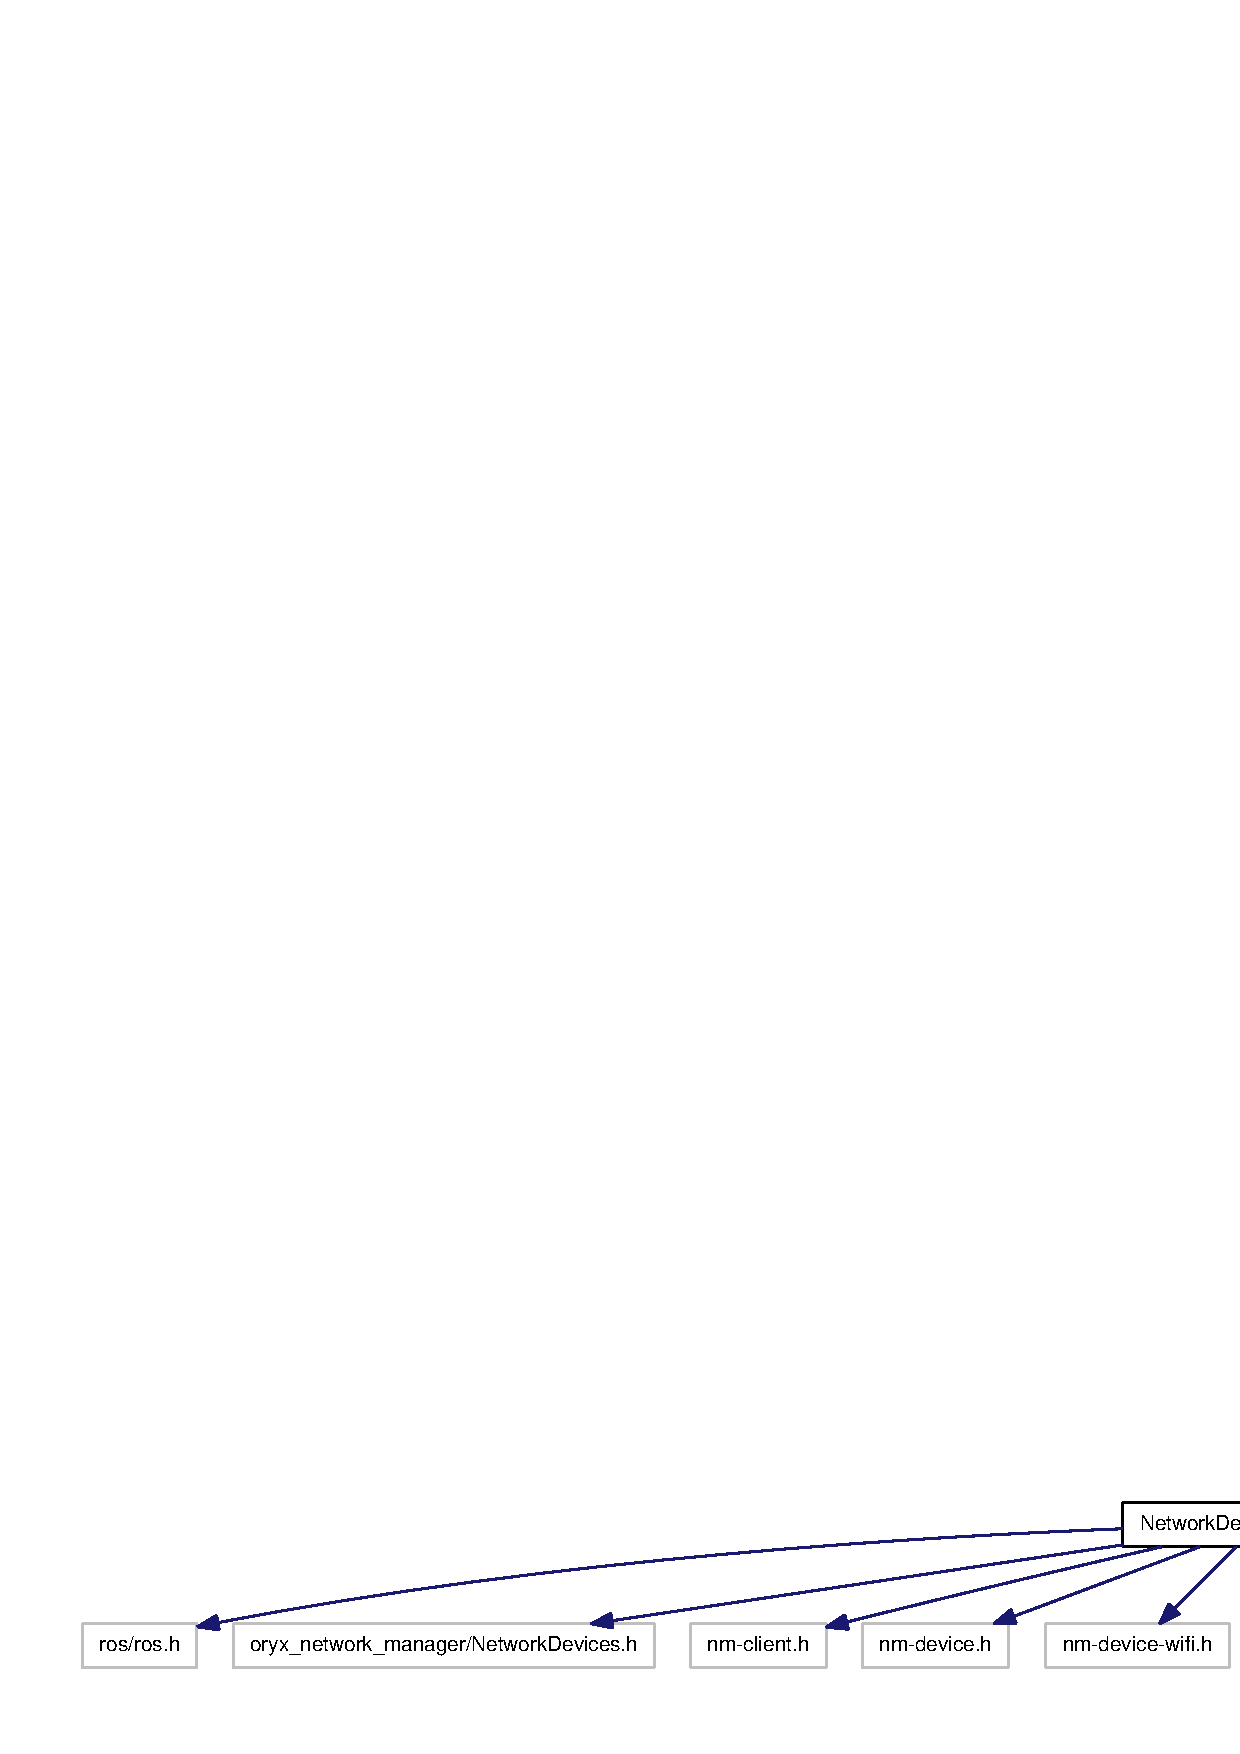
\includegraphics[width=350pt]{NetworkDeviceManager_8cpp__incl}
\end{center}
\end{figure}

\section{\-Network\-Device\-Manager.\-h \-File \-Reference}
\label{NetworkDeviceManager_8h}\index{\-Network\-Device\-Manager.\-h@{\-Network\-Device\-Manager.\-h}}
{\ttfamily \#include \char`\"{}ros/ros.\-h\char`\"{}}\*
{\ttfamily \#include \char`\"{}oryx\-\_\-network\-\_\-manager/\-Network\-Devices.\-h\char`\"{}}\*
{\ttfamily \#include $<$nm-\/client.\-h$>$}\*
{\ttfamily \#include $<$nm-\/device.\-h$>$}\*
{\ttfamily \#include $<$nm-\/device-\/wifi.\-h$>$}\*
{\ttfamily \#include $<$nm-\/device-\/ethernet.\-h$>$}\*
{\ttfamily \#include $<$nm-\/device-\/modem.\-h$>$}\*
{\ttfamily \#include $<$nm-\/device-\/wimax.\-h$>$}\*
{\ttfamily \#include $<$map$>$}\*
\-Include dependency graph for \-Network\-Device\-Manager.\-h\-:
\nopagebreak
\begin{figure}[H]
\begin{center}
\leavevmode
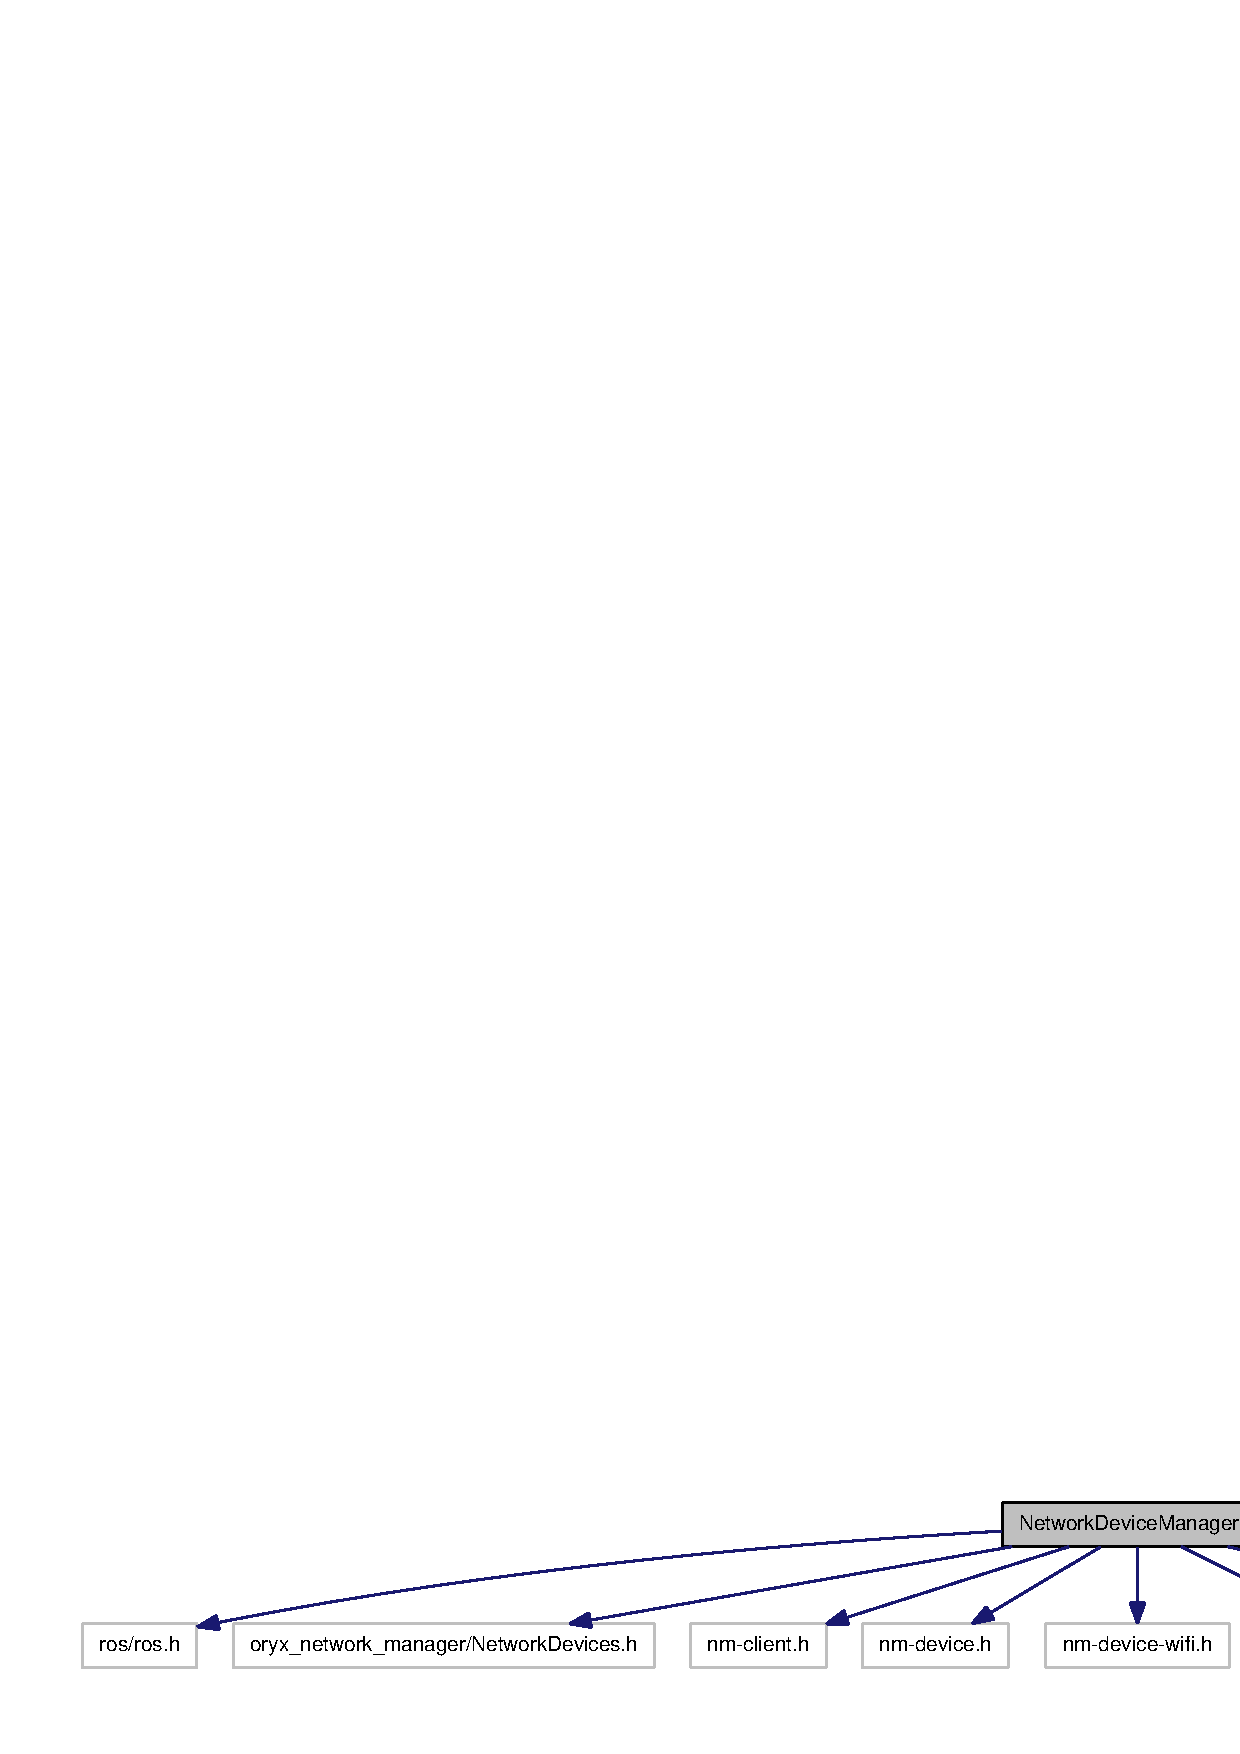
\includegraphics[width=350pt]{NetworkDeviceManager_8h__incl}
\end{center}
\end{figure}
\-This graph shows which files directly or indirectly include this file\-:
\nopagebreak
\begin{figure}[H]
\begin{center}
\leavevmode
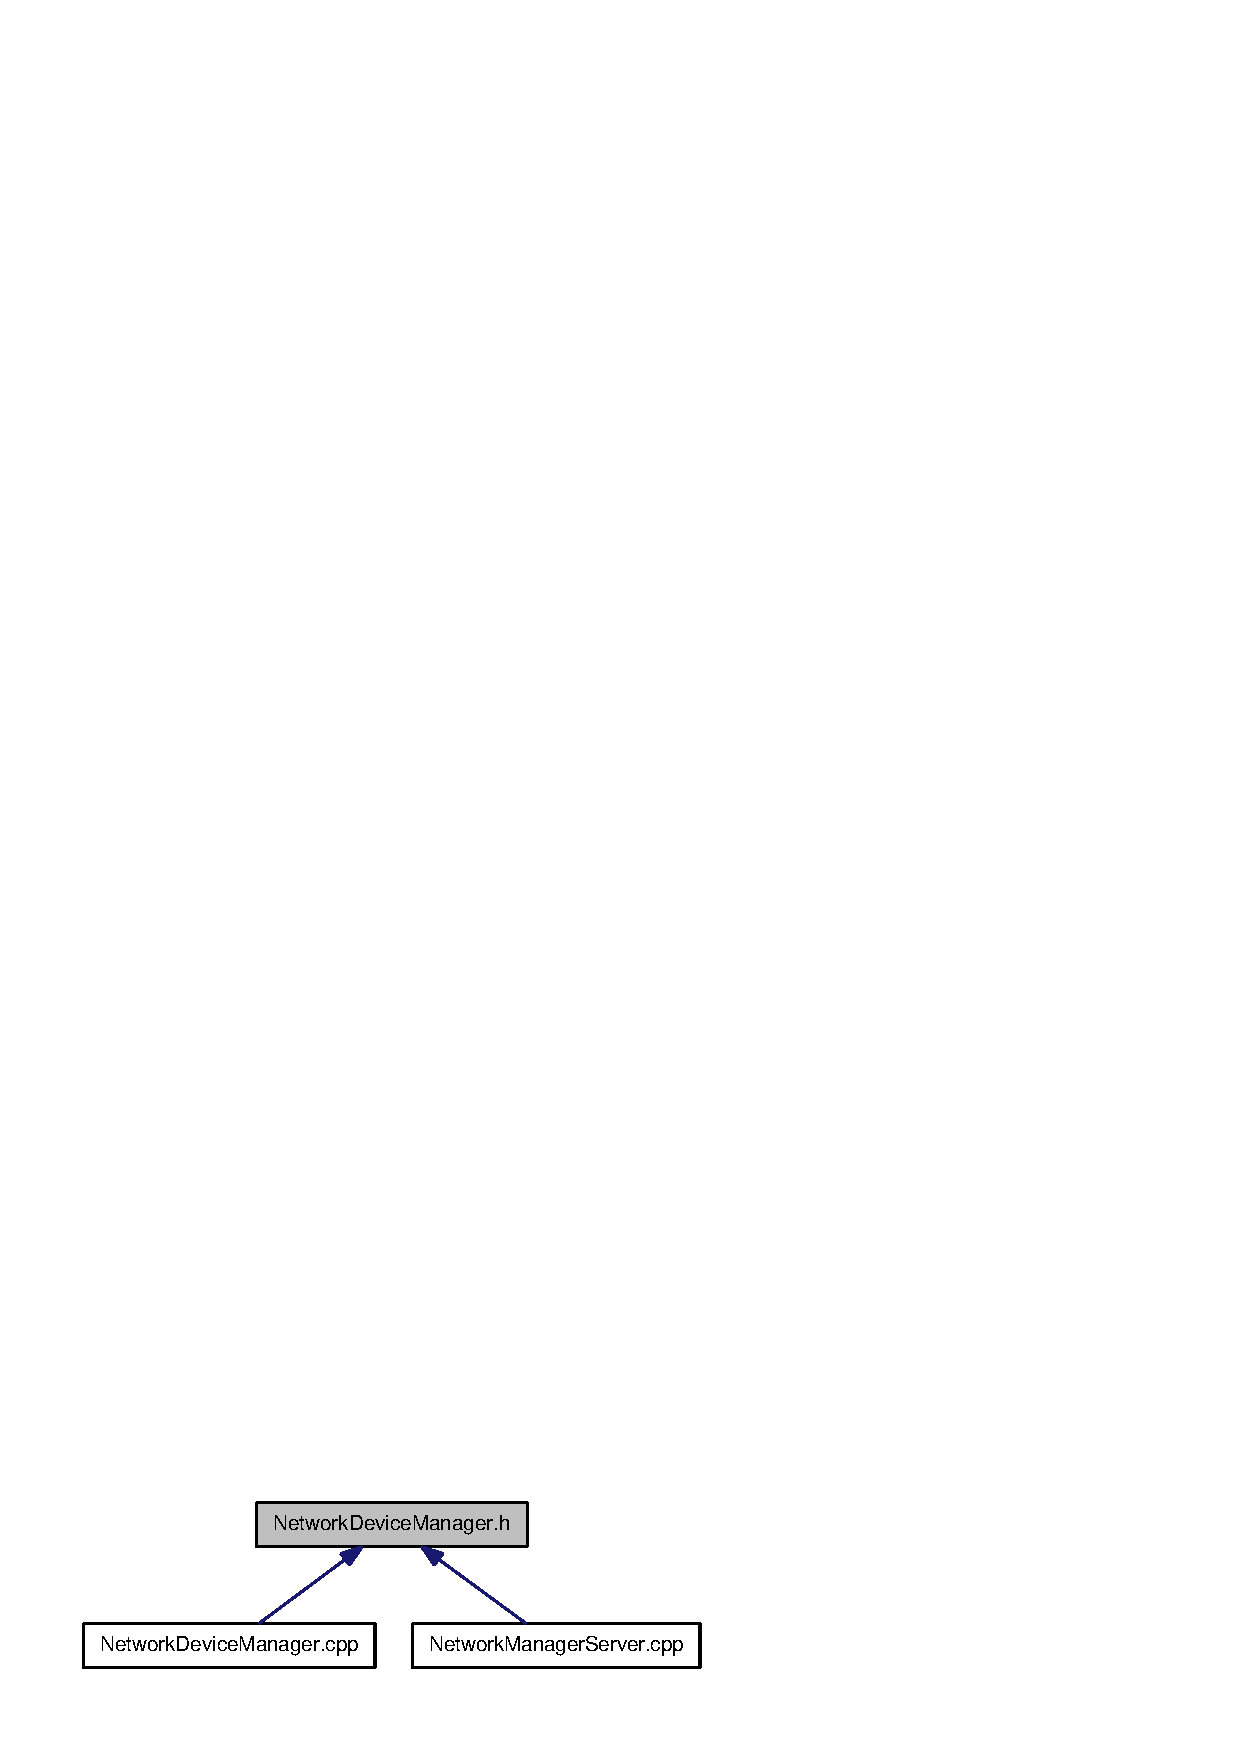
\includegraphics[width=340pt]{NetworkDeviceManager_8h__dep__incl}
\end{center}
\end{figure}
\subsection*{\-Classes}
\begin{DoxyCompactItemize}
\item 
class {\bf \-Network\-Device\-Manager}
\end{DoxyCompactItemize}

\section{\-Network\-Manager\-C\-L\-I.\-cpp \-File \-Reference}
\label{NetworkManagerCLI_8cpp}\index{\-Network\-Manager\-C\-L\-I.\-cpp@{\-Network\-Manager\-C\-L\-I.\-cpp}}
{\ttfamily \#include \char`\"{}ros/ros.\-h\char`\"{}}\*
{\ttfamily \#include \char`\"{}oryx\-\_\-network\-\_\-manager/\-Network\-Connections.\-h\char`\"{}}\*
{\ttfamily \#include \char`\"{}oryx\-\_\-network\-\_\-manager/\-Network\-Devices.\-h\char`\"{}}\*
{\ttfamily \#include \char`\"{}oryx\-\_\-network\-\_\-manager/\-Active\-Network\-Connections.\-h\char`\"{}}\*
{\ttfamily \#include \char`\"{}oryx\-\_\-network\-\_\-manager/\-Activate\-Connection.\-h\char`\"{}}\*
{\ttfamily \#include $<$sstream$>$}\*
\-Include dependency graph for \-Network\-Manager\-C\-L\-I.\-cpp\-:
\nopagebreak
\begin{figure}[H]
\begin{center}
\leavevmode
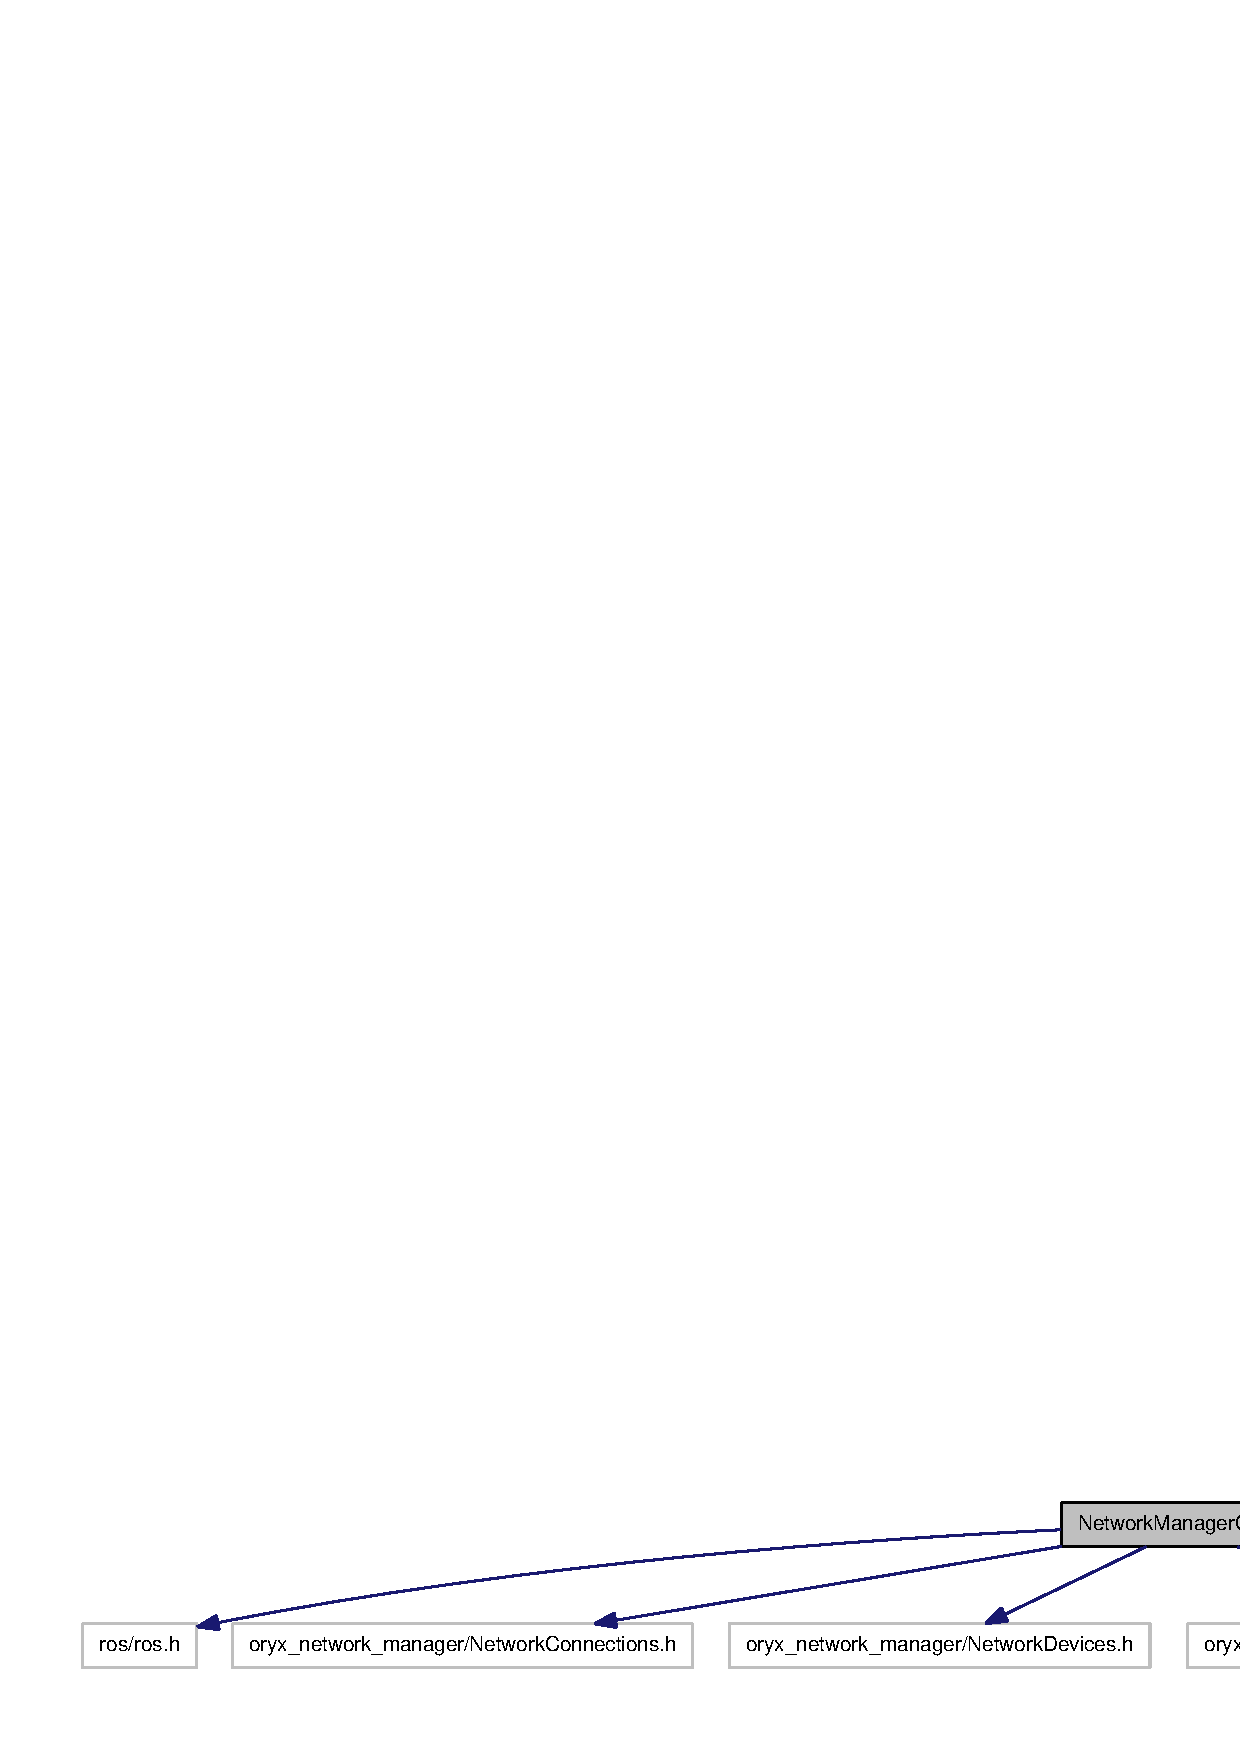
\includegraphics[width=350pt]{NetworkManagerCLI_8cpp__incl}
\end{center}
\end{figure}
\subsection*{\-Functions}
\begin{DoxyCompactItemize}
\item 
void {\bf connect} (const char $\ast$iface, const char $\ast$connection\-\_\-name)
\item 
void {\bf help} (const char $\ast$message)
\item 
void {\bf list\-\_\-active\-\_\-connections} (bool run\-\_\-once)
\item 
void {\bf list\-\_\-active\-\_\-connections\-\_\-callback} (const \-Active\-Network\-Connections\-::\-Const\-Ptr \&active\-\_\-connections, bool run\-\_\-once)
\item 
void {\bf list\-\_\-connections} (bool run\-\_\-once)
\item 
void {\bf list\-\_\-connections\-\_\-callback} (const \-Network\-Connections\-::\-Const\-Ptr \&connections, bool run\-\_\-once)
\item 
void {\bf list\-\_\-devices} (bool run\-\_\-once)
\item 
void {\bf list\-\_\-devices\-\_\-callback} (const \-Network\-Devices\-::\-Const\-Ptr \&devices, bool run\-\_\-once)
\item 
int {\bf main} (int argc, char $\ast$$\ast$argv)
\end{DoxyCompactItemize}


\subsection{\-Function \-Documentation}
\index{\-Network\-Manager\-C\-L\-I.\-cpp@{\-Network\-Manager\-C\-L\-I.\-cpp}!connect@{connect}}
\index{connect@{connect}!NetworkManagerCLI.cpp@{\-Network\-Manager\-C\-L\-I.\-cpp}}
\subsubsection[{connect}]{\setlength{\rightskip}{0pt plus 5cm}void {\bf connect} (
\begin{DoxyParamCaption}
\item[{const char $\ast$}]{iface, }
\item[{const char $\ast$}]{connection\-\_\-name}
\end{DoxyParamCaption}
)}\label{NetworkManagerCLI_8cpp_aeed3893b8ce500d2f9c7d4f12a6b8ff6}


\-Definition at line 100 of file \-Network\-Manager\-C\-L\-I.\-cpp.

\index{\-Network\-Manager\-C\-L\-I.\-cpp@{\-Network\-Manager\-C\-L\-I.\-cpp}!help@{help}}
\index{help@{help}!NetworkManagerCLI.cpp@{\-Network\-Manager\-C\-L\-I.\-cpp}}
\subsubsection[{help}]{\setlength{\rightskip}{0pt plus 5cm}void {\bf help} (
\begin{DoxyParamCaption}
\item[{const char $\ast$}]{message}
\end{DoxyParamCaption}
)}\label{NetworkManagerCLI_8cpp_a73fe081479888fcd619a52229be228a5}


\-Definition at line 115 of file \-Network\-Manager\-C\-L\-I.\-cpp.

\index{\-Network\-Manager\-C\-L\-I.\-cpp@{\-Network\-Manager\-C\-L\-I.\-cpp}!list\-\_\-active\-\_\-connections@{list\-\_\-active\-\_\-connections}}
\index{list\-\_\-active\-\_\-connections@{list\-\_\-active\-\_\-connections}!NetworkManagerCLI.cpp@{\-Network\-Manager\-C\-L\-I.\-cpp}}
\subsubsection[{list\-\_\-active\-\_\-connections}]{\setlength{\rightskip}{0pt plus 5cm}void {\bf list\-\_\-active\-\_\-connections} (
\begin{DoxyParamCaption}
\item[{bool}]{run\-\_\-once}
\end{DoxyParamCaption}
)}\label{NetworkManagerCLI_8cpp_a91ab5129d8f7c29f5ceac523f5b952c7}


\-Definition at line 65 of file \-Network\-Manager\-C\-L\-I.\-cpp.

\index{\-Network\-Manager\-C\-L\-I.\-cpp@{\-Network\-Manager\-C\-L\-I.\-cpp}!list\-\_\-active\-\_\-connections\-\_\-callback@{list\-\_\-active\-\_\-connections\-\_\-callback}}
\index{list\-\_\-active\-\_\-connections\-\_\-callback@{list\-\_\-active\-\_\-connections\-\_\-callback}!NetworkManagerCLI.cpp@{\-Network\-Manager\-C\-L\-I.\-cpp}}
\subsubsection[{list\-\_\-active\-\_\-connections\-\_\-callback}]{\setlength{\rightskip}{0pt plus 5cm}void {\bf list\-\_\-active\-\_\-connections\-\_\-callback} (
\begin{DoxyParamCaption}
\item[{const \-Active\-Network\-Connections\-::\-Const\-Ptr \&}]{active\-\_\-connections, }
\item[{bool}]{run\-\_\-once}
\end{DoxyParamCaption}
)}\label{NetworkManagerCLI_8cpp_aa50884b1f3d4fe36b7d9eeeec136516c}


\-Definition at line 49 of file \-Network\-Manager\-C\-L\-I.\-cpp.

\index{\-Network\-Manager\-C\-L\-I.\-cpp@{\-Network\-Manager\-C\-L\-I.\-cpp}!list\-\_\-connections@{list\-\_\-connections}}
\index{list\-\_\-connections@{list\-\_\-connections}!NetworkManagerCLI.cpp@{\-Network\-Manager\-C\-L\-I.\-cpp}}
\subsubsection[{list\-\_\-connections}]{\setlength{\rightskip}{0pt plus 5cm}void {\bf list\-\_\-connections} (
\begin{DoxyParamCaption}
\item[{bool}]{run\-\_\-once}
\end{DoxyParamCaption}
)}\label{NetworkManagerCLI_8cpp_ac5db45ad2db212a13f79df665ea377c4}


\-Definition at line 41 of file \-Network\-Manager\-C\-L\-I.\-cpp.

\index{\-Network\-Manager\-C\-L\-I.\-cpp@{\-Network\-Manager\-C\-L\-I.\-cpp}!list\-\_\-connections\-\_\-callback@{list\-\_\-connections\-\_\-callback}}
\index{list\-\_\-connections\-\_\-callback@{list\-\_\-connections\-\_\-callback}!NetworkManagerCLI.cpp@{\-Network\-Manager\-C\-L\-I.\-cpp}}
\subsubsection[{list\-\_\-connections\-\_\-callback}]{\setlength{\rightskip}{0pt plus 5cm}void {\bf list\-\_\-connections\-\_\-callback} (
\begin{DoxyParamCaption}
\item[{const \-Network\-Connections\-::\-Const\-Ptr \&}]{connections, }
\item[{bool}]{run\-\_\-once}
\end{DoxyParamCaption}
)}\label{NetworkManagerCLI_8cpp_ac404438ec9bd52c3a6f43a6815bdbf60}


\-Definition at line 20 of file \-Network\-Manager\-C\-L\-I.\-cpp.

\index{\-Network\-Manager\-C\-L\-I.\-cpp@{\-Network\-Manager\-C\-L\-I.\-cpp}!list\-\_\-devices@{list\-\_\-devices}}
\index{list\-\_\-devices@{list\-\_\-devices}!NetworkManagerCLI.cpp@{\-Network\-Manager\-C\-L\-I.\-cpp}}
\subsubsection[{list\-\_\-devices}]{\setlength{\rightskip}{0pt plus 5cm}void {\bf list\-\_\-devices} (
\begin{DoxyParamCaption}
\item[{bool}]{run\-\_\-once}
\end{DoxyParamCaption}
)}\label{NetworkManagerCLI_8cpp_ae00ec5aec66a1a7e48745a98891ef272}


\-Definition at line 92 of file \-Network\-Manager\-C\-L\-I.\-cpp.

\index{\-Network\-Manager\-C\-L\-I.\-cpp@{\-Network\-Manager\-C\-L\-I.\-cpp}!list\-\_\-devices\-\_\-callback@{list\-\_\-devices\-\_\-callback}}
\index{list\-\_\-devices\-\_\-callback@{list\-\_\-devices\-\_\-callback}!NetworkManagerCLI.cpp@{\-Network\-Manager\-C\-L\-I.\-cpp}}
\subsubsection[{list\-\_\-devices\-\_\-callback}]{\setlength{\rightskip}{0pt plus 5cm}void {\bf list\-\_\-devices\-\_\-callback} (
\begin{DoxyParamCaption}
\item[{const \-Network\-Devices\-::\-Const\-Ptr \&}]{devices, }
\item[{bool}]{run\-\_\-once}
\end{DoxyParamCaption}
)}\label{NetworkManagerCLI_8cpp_a5767123336e76e31bf9fb9d064096a8f}


\-Definition at line 73 of file \-Network\-Manager\-C\-L\-I.\-cpp.

\index{\-Network\-Manager\-C\-L\-I.\-cpp@{\-Network\-Manager\-C\-L\-I.\-cpp}!main@{main}}
\index{main@{main}!NetworkManagerCLI.cpp@{\-Network\-Manager\-C\-L\-I.\-cpp}}
\subsubsection[{main}]{\setlength{\rightskip}{0pt plus 5cm}int {\bf main} (
\begin{DoxyParamCaption}
\item[{int}]{argc, }
\item[{char $\ast$$\ast$}]{argv}
\end{DoxyParamCaption}
)}\label{NetworkManagerCLI_8cpp_a3c04138a5bfe5d72780bb7e82a18e627}


\-Definition at line 129 of file \-Network\-Manager\-C\-L\-I.\-cpp.


\section{\-Network\-Manager\-Server.\-cpp \-File \-Reference}
\label{NetworkManagerServer_8cpp}\index{\-Network\-Manager\-Server.\-cpp@{\-Network\-Manager\-Server.\-cpp}}
{\ttfamily \#include $<$stdio.\-h$>$}\*
{\ttfamily \#include $<$stdlib.\-h$>$}\*
{\ttfamily \#include \char`\"{}ros/ros.\-h\char`\"{}}\*
{\ttfamily \#include $<$glib.\-h$>$}\*
{\ttfamily \#include $<$dbus/dbus-\/glib.\-h$>$}\*
{\ttfamily \#include $<$dbus/dbus.\-h$>$}\*
{\ttfamily \#include $<$pthread.\-h$>$}\*
{\ttfamily \#include \char`\"{}\-Network\-Device\-Manager.\-h\char`\"{}}\*
{\ttfamily \#include \char`\"{}\-Network\-Connection\-Manager.\-h\char`\"{}}\*
{\ttfamily \#include \char`\"{}\-Active\-Network\-Connection\-Manager.\-h\char`\"{}}\*
{\ttfamily \#include \char`\"{}\-Activate\-Connection\-Service.\-h\char`\"{}}\*
{\ttfamily \#include \char`\"{}\-Network\-Configuration\-Manager.\-h\char`\"{}}\*
\-Include dependency graph for \-Network\-Manager\-Server.\-cpp\-:
\nopagebreak
\begin{figure}[H]
\begin{center}
\leavevmode
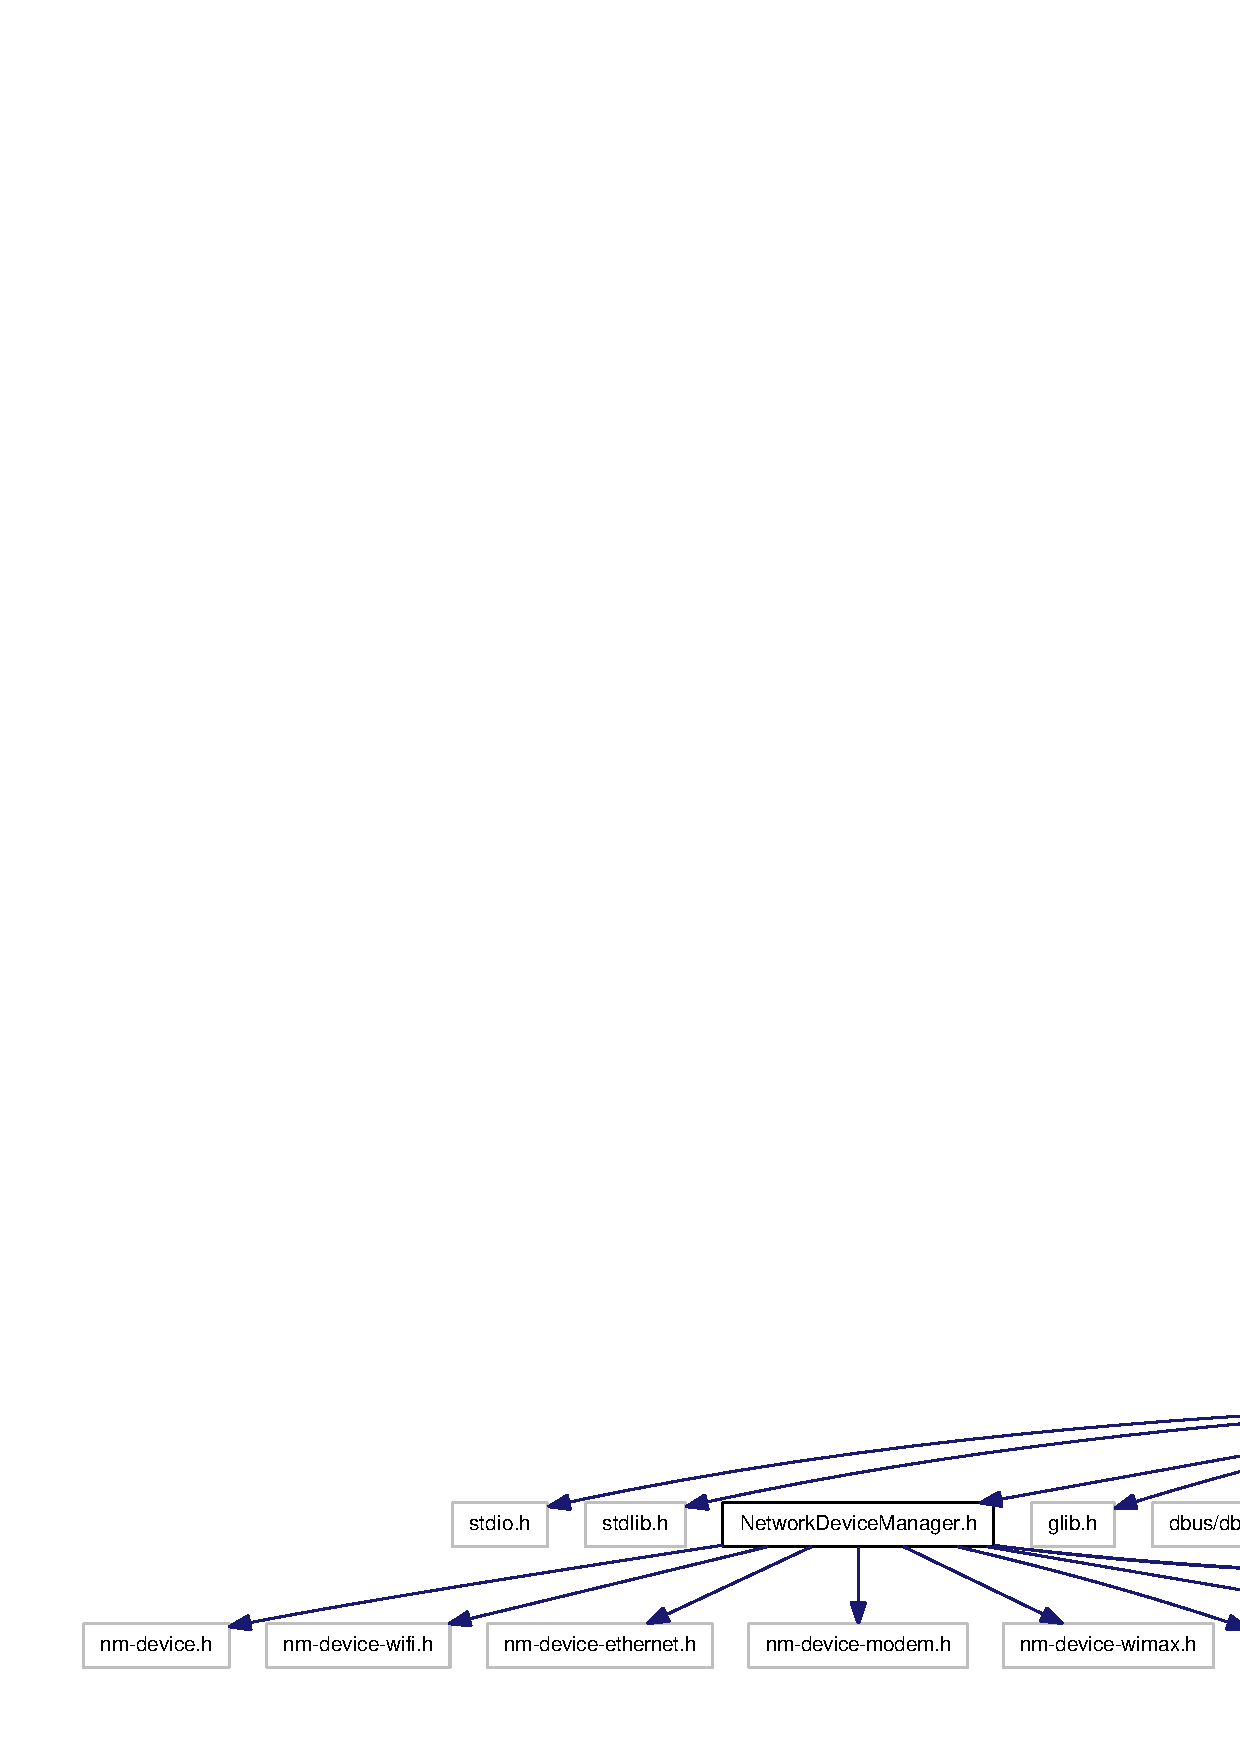
\includegraphics[width=350pt]{NetworkManagerServer_8cpp__incl}
\end{center}
\end{figure}
\subsection*{\-Functions}
\begin{DoxyCompactItemize}
\item 
void {\bf got\-\_\-connections\-\_\-cb} ()
\item 
int {\bf main} (int argc, char $\ast$$\ast$argv)
\item 
static void $\ast$ {\bf run\-\_\-main\-\_\-loop} (void $\ast$loop)
\item 
static void {\bf spawn\-\_\-g\-\_\-main\-\_\-loop} (\-G\-Main\-Loop $\ast$loop)
\end{DoxyCompactItemize}
\subsection*{\-Variables}
\begin{DoxyCompactItemize}
\item 
pthread\-\_\-t {\bf g\-\_\-main\-\_\-loop\-\_\-thread}
\end{DoxyCompactItemize}


\subsection{\-Function \-Documentation}
\index{\-Network\-Manager\-Server.\-cpp@{\-Network\-Manager\-Server.\-cpp}!got\-\_\-connections\-\_\-cb@{got\-\_\-connections\-\_\-cb}}
\index{got\-\_\-connections\-\_\-cb@{got\-\_\-connections\-\_\-cb}!NetworkManagerServer.cpp@{\-Network\-Manager\-Server.\-cpp}}
\subsubsection[{got\-\_\-connections\-\_\-cb}]{\setlength{\rightskip}{0pt plus 5cm}void {\bf got\-\_\-connections\-\_\-cb} (
\begin{DoxyParamCaption}
{}
\end{DoxyParamCaption}
)}\label{NetworkManagerServer_8cpp_a7d4b9bdeb3e107efe5fb7b01bca560cf}


\-Definition at line 43 of file \-Network\-Manager\-Server.\-cpp.

\index{\-Network\-Manager\-Server.\-cpp@{\-Network\-Manager\-Server.\-cpp}!main@{main}}
\index{main@{main}!NetworkManagerServer.cpp@{\-Network\-Manager\-Server.\-cpp}}
\subsubsection[{main}]{\setlength{\rightskip}{0pt plus 5cm}int {\bf main} (
\begin{DoxyParamCaption}
\item[{int}]{argc, }
\item[{char $\ast$$\ast$}]{argv}
\end{DoxyParamCaption}
)}\label{NetworkManagerServer_8cpp_a3c04138a5bfe5d72780bb7e82a18e627}


\-Definition at line 47 of file \-Network\-Manager\-Server.\-cpp.

\index{\-Network\-Manager\-Server.\-cpp@{\-Network\-Manager\-Server.\-cpp}!run\-\_\-main\-\_\-loop@{run\-\_\-main\-\_\-loop}}
\index{run\-\_\-main\-\_\-loop@{run\-\_\-main\-\_\-loop}!NetworkManagerServer.cpp@{\-Network\-Manager\-Server.\-cpp}}
\subsubsection[{run\-\_\-main\-\_\-loop}]{\setlength{\rightskip}{0pt plus 5cm}static void$\ast$ {\bf run\-\_\-main\-\_\-loop} (
\begin{DoxyParamCaption}
\item[{void $\ast$}]{loop}
\end{DoxyParamCaption}
)\hspace{0.3cm}{\ttfamily  [static]}}\label{NetworkManagerServer_8cpp_a399da051f4f2766856947a4d5a9ac534}


\-Definition at line 25 of file \-Network\-Manager\-Server.\-cpp.

\index{\-Network\-Manager\-Server.\-cpp@{\-Network\-Manager\-Server.\-cpp}!spawn\-\_\-g\-\_\-main\-\_\-loop@{spawn\-\_\-g\-\_\-main\-\_\-loop}}
\index{spawn\-\_\-g\-\_\-main\-\_\-loop@{spawn\-\_\-g\-\_\-main\-\_\-loop}!NetworkManagerServer.cpp@{\-Network\-Manager\-Server.\-cpp}}
\subsubsection[{spawn\-\_\-g\-\_\-main\-\_\-loop}]{\setlength{\rightskip}{0pt plus 5cm}static void {\bf spawn\-\_\-g\-\_\-main\-\_\-loop} (
\begin{DoxyParamCaption}
\item[{\-G\-Main\-Loop $\ast$}]{loop}
\end{DoxyParamCaption}
)\hspace{0.3cm}{\ttfamily  [static]}}\label{NetworkManagerServer_8cpp_a8a9855b1c32e1e915b3d5a32f331ed74}


\-Definition at line 34 of file \-Network\-Manager\-Server.\-cpp.



\subsection{\-Variable \-Documentation}
\index{\-Network\-Manager\-Server.\-cpp@{\-Network\-Manager\-Server.\-cpp}!g\-\_\-main\-\_\-loop\-\_\-thread@{g\-\_\-main\-\_\-loop\-\_\-thread}}
\index{g\-\_\-main\-\_\-loop\-\_\-thread@{g\-\_\-main\-\_\-loop\-\_\-thread}!NetworkManagerServer.cpp@{\-Network\-Manager\-Server.\-cpp}}
\subsubsection[{g\-\_\-main\-\_\-loop\-\_\-thread}]{\setlength{\rightskip}{0pt plus 5cm}pthread\-\_\-t {\bf g\-\_\-main\-\_\-loop\-\_\-thread}}\label{NetworkManagerServer_8cpp_a33a37394f9142e45773417cd32f8c5bd}


\-Definition at line 23 of file \-Network\-Manager\-Server.\-cpp.


\printindex
\end{document}
